% https://github.com/cohomolo-gy/cats-in-context/blob/master/chapter-2/Chapter%202%20Solutions.tex

\documentclass[14pt]{report}
\usepackage{classicthesis}

\usepackage{bbm}
\usepackage{bbding} % for flower. 
\usepackage{physics}
\usepackage{amsmath,amssymb}
\usepackage{graphicx}
\usepackage{makeidx}
\usepackage{algpseudocode}
\usepackage{algorithm}
\usepackage{listing}
\usepackage{minted}
\usepackage{cancel}
\usepackage{color}% or xcolor
\usepackage{quiver}
\usepackage{changepage}
\usepackage{booktabs}   %% For formal tables:
                        %% http://ctan.org/pkg/booktabs
\usepackage{subcaption} %% For complex figures with subfigures/subcaptions
                        %% http://ctan.org/pkg/subcaption
\usepackage{enumitem}
\usepackage{mathtools}
%\usepackage{minted}
%\newminted{fortran}{fontsize=\footnotesize}

\usepackage{xargs}
\usepackage[colorinlistoftodos,prependcaption,textsize=tiny]{todonotes}

\usepackage{hyperref}
\hypersetup{
    colorlinks,
    citecolor=blue,
    filecolor=blue,
    linkcolor=blue,
    urlcolor=blue
}

\usepackage{epsfig}
\usepackage{tabularx}
\usepackage{latexsym}
\newcommand\ddfrac[2]{\frac{\displaystyle #1}{\displaystyle #2}}
\newcommand{\N}{\ensuremath{\mathbb{N}}}
\newcommand{\Z}{\ensuremath{\mathbb{Z}}}
\newcommand{\Q}{\ensuremath{\mathbb{Q}}}
\newcommand{\R}{\ensuremath{\mathbb R}}
\newcommand{\coT}{\ensuremath{T^*}}
\newcommand{\boldX}{\ensuremath{\mathbf{X}}}
\newcommand{\boldY}{\ensuremath{\mathbf{Y}}}


\newcommand{\cat}[1]{\mathsf{#1}}
\newcommand{\functor}[3]{#1 : \cat{#2} \to \cat{#3}}
\newcommand{\functordef}{\functor{F}{C}{D}}
\newcommand{\cc}{\cat{C}}
\newcommand{\cC}{\cat{C}}
\renewcommand{\dd}{\cat{D}}
\newcommand{\ee}{\cat{E}}
\newcommand{\ccat}{\cat{Cat}}
\newcommand{\cCat}{\cat{Cat}}
\newcommand{\cset}{\cat{Set}}
\newcommand{\cSet}{\cat{Set}}
\newcommand{\cFin}{\cat{Fin}}
\newcommand{\cCAT}{\cat{CAT}}
\newcommand{\cTop}{\cat{Top}}
\newcommand{\ctop}{\cat{Top}}
\newcommand{\cgrp}{\cat{Grp}}
\newcommand{\cGrp}{\cat{Grp}}
\newcommand{\cCone}{\cat{Cone}}

\newcommand{\subcat}[2]{\bm{ \mathsf{#1}}_{\bm{ \mathsf{#2}}}}
\renewcommand{\op}{\text{op}}
\newcommand{\inv}[1]{#1^{-1}}
\newcommand{\mono}{\rightarrowtail}
\newcommand{\epi}{\twoheadrightarrow}
\newcommand{\bg}{\cat{BG}}
\newcommand{\bgg}{\cat{BG'}}
\newcommand{\nt}{\Rightarrow}
%\newcommand{\ant}[2]{\alpha : F \nt G} 
%\newcommand{\bnt}[2]{\beta : F \nt G} 
%\newcommand{\anti}[2]{\alpha : F \cong G} 
%\newcommand{\bnti}[2]{\beta : F \cong G} 
\newcommand{\zero}{\mathbbm{0}}
\newcommand{\one}{\mathbbm{1}}
\newcommand{\two}{\mathbbm{2}}
\newcommand{\three}{\mathbbm{3}}
\newcommand{\id}{\operatorname{id}}
\newcommand{\Id}{\operatorname{id}}
\newcommand{\colim}{\operatorname{colim}}



\newcommand{\G}{\ensuremath{\mathcal{G}}}
% \newcommand{\braket}[2]{\ensuremath{\left\langle #1 \vert #2 \right\rangle}}


\def\qed{$\Box$}
\newtheorem{theorem}{Theorem}
\newtheorem{corollary}[theorem]{Corollary}
\newtheorem{definition}[theorem]{Definition}
\newtheorem{lemma}[theorem]{Lemma}
\newtheorem{observation}[theorem]{Observation}
\newtheorem{remark}[theorem]{Remark}
\newtheorem{example}[theorem]{Example}
\newtheorem{exercise}[theorem]{Exercise}
 
% \newcommand{\proof}[1][]{\emph{Proof #1}\textbf{:} }
\newcommand*{\start}[1]{\leavevmode\newline \textbf{#1} }
\newcommand*{\question}[1]{\leavevmode\newline \par\noindent\rule{\textwidth}{0.4pt} \textbf{Question: #1.}}
\newcommand*{\proof}[1]{\leavevmode\newline \textbf{Proof #1}}
\newcommand*{\answer}{\leavevmode\newline \textbf{Answer} }

\newcommand{\X}{\ensuremath{\mathfrak{X}}}
\newcommand{\comma}{\downarrow}


% \newcommand{\hom}{\ensuremath{\operatorname{Hom}}}
\newcommand{\Hom}{\ensuremath{\operatorname{Hom}}}

\title{Category theory in context}
\author{Siddharth Bhat}
\date{Monsoon, second year of the plague}


\begin{document}
\maketitle
\tableofcontents
\chapter{Categories, Functors, Natural transformations}
\section{Abstract and concrete categories}
\section{Duality}
\subsection{Musing}
How does one remember mono is is $gk = gl \implies k = l$ and vice versa?

\subsection{Solutions}
\question{Lemma 1.2.3} $f: x \to y$ is an isomorphism iff it defines a bijection $f_*: C(c, x) \to C(c, y)$.


\proof[($f$ is iso $\implies$ post composition with $f$ induces bijection)]
Let $f: x \to y$ be an isomorphism. Thus we have an inverse arrow $g: y \to x$ such that $fg = id_y$, $gf = id_x$.
The map: $$C(c, x) \xrightarrow{f*} C(c, y): (\alpha: c \to x) \mapsto (f\alpha: c \to y)$$
has a two sided inverse:

$$
C(c, y) \xrightarrow{g*} C(c, x): (\beta: c \to y) \mapsto (g\beta: c \to x)
$$

which can be checked as $g_*(f_*(\alpha)) = g_*(f\alpha) = gf\alpha = id_x\alpha = \alpha$, and similarly for $f_*(g_*(\beta))$.
Hence we are done, as the iso induces a bijection of hom-sets.
\qed


\proof[(post-composition with $f$ is bijection implies $f$ is iso)]
We are given that the post composition by $f$, $f_*: C(c, x) \rightarrow C(c, y)$ is a bijection.
We need to show that $f$ is an isomorphism, which means that there exists a function $g$ such that $fg = id_y$ and $gf = id_x$.
Since post-composition is a bijection for all $c$, pick $c = y$. This tells us that the post-composition 
$f_*: C(y, x) \rightarrow C(y, y)$ is a bijection. Since $id_y \in C(y, y)$, $id_y$ an inverse image $g \equiv f_*^{-1}(id_y)$. 
[We choose to call this map $g$]. By definition of $f_*^{-1}$, we have that $f_*(f_*^{-1}(id_y)) = id_y$ , which means
that $fg = id_y$. We also need to show that $gf = id_x$. To show this, consider $f_*(gf) = fgf = (fg)f = (1_y)f = f$.
We also have that $f_*(id_x) = f id_x = f$. Since $f_*$ is a bijection, we have that $id_x = gf$ and we are done.  \qed


\begin{minipage}{\textwidth}
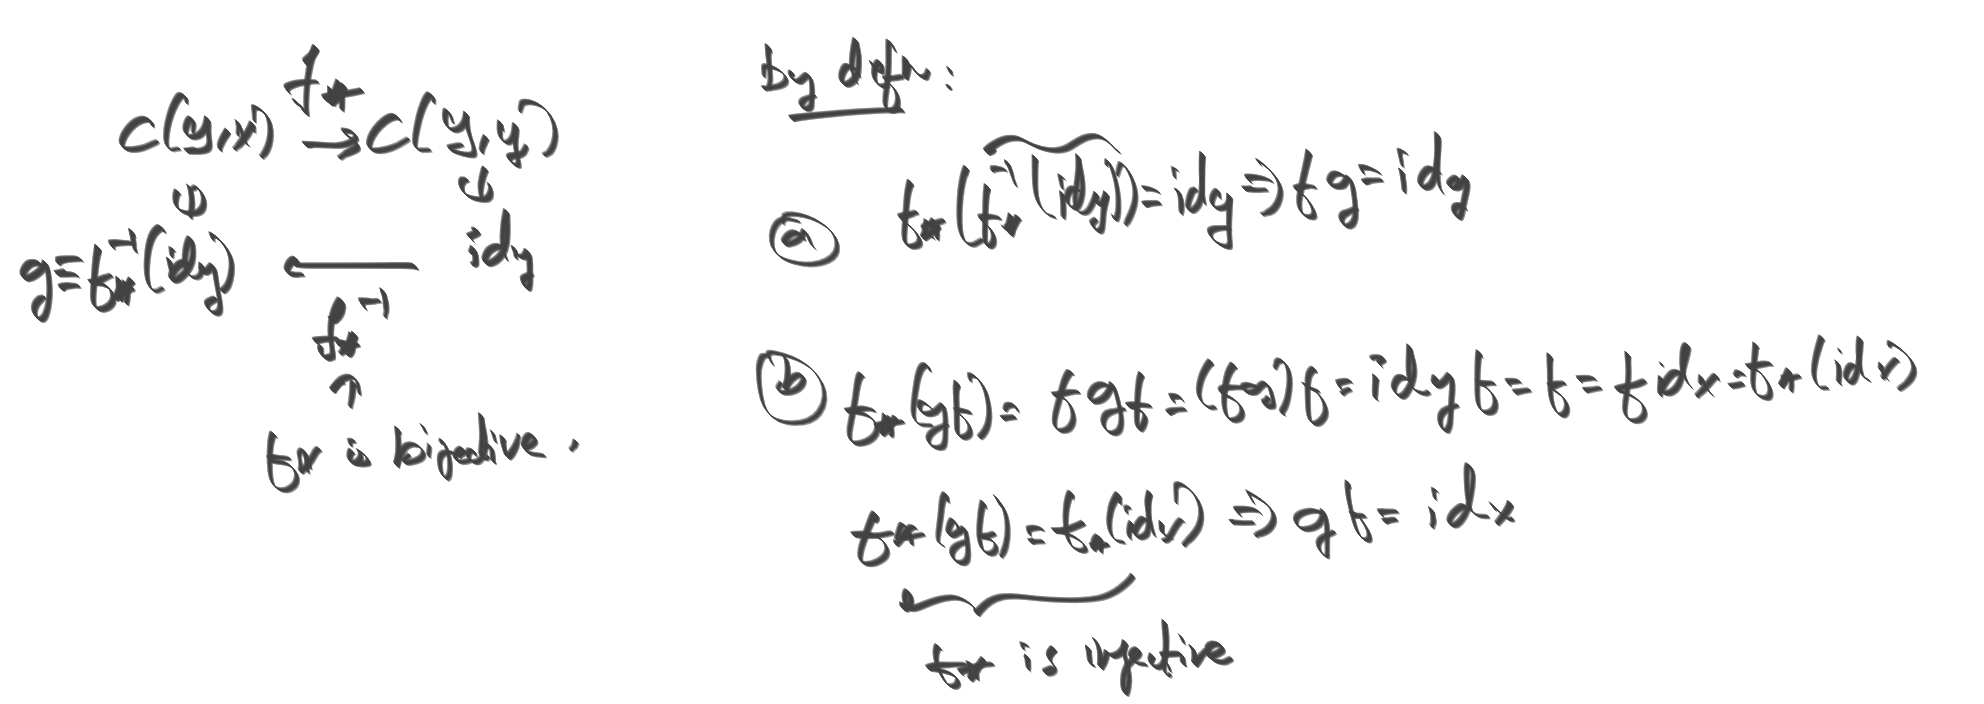
\includegraphics[width=\textwidth]{ch1/iso-is-bijection-of-hom.png}
    \begin{center}Iso is bijection of hom-sets\end{center}
\end{minipage}

\question{Q 1.2.ii:} Show that $f: x \rightarrow y$ is split epi iff for all $c \in C$, post composition
$f \circ - : C(c, x) \rightarrow C(c, y)$ is a surjection.


\proof[(split epi implies post composition is surjective)]
Let $f: e \rightarrow b$ be split epi, and thus possess a section $s: b \rightarrow e$ such that $fs = id_b$.
We wish to show that post composition $C(c, e) \xrightarrow{f_*} C(c, b)$ is surjective.
So pick any $g \in C(c, b)$. Define $sg \in C(c, e)$. See: $$f_*(sg) = fsg = (fs)g = id_b g = g$$.
Hence, for all $g \in C(c, b)$ there exists a pre-image under $f_*$, $sg \in C(c, e)$. Thus, $f_*$ is surjective
since every element of codomain has a pre-image. \qed


\proof[(post composition is surjective implies split epi)]
Let $f: e \to b$ be a morphism such that for all $c \in C$, we have $C(c, e) \xrightarrow{f_*} C(c, b)$ is surjective.
We need to show that there exists a morpshism $s: b \rightarrow e$ such that $fs = id_b$. Set $c = b$.
This gives us a surjection $C(b, e) \xrightarrow{f_*} C(b, b)$. Pick an inverse image of $id_b \in C(b, b)$. 
That is, pick any function $s \in f_*^{-1}(id_b)$. By definition, of $s$ being in the fiber of $id_b$,
we have that $f_*(s) = fs = id_b$. Thus means that we have found a function $s$ such that $fs = id_b$. Thus we are done.
\qed

\question{Q 1.2.iii:} Mono is closed under composition, and if $gf$ is monic then so is $f$.


\proof[(Mono is closed under composition)]
Let $f: x \to y, g: y \to z$ be monomorphisms (Recall that $f$ is a monomorphism iff for any $\alpha, \beta$, if $f \alpha = f \beta$ then $\alpha = \beta$).
We are to show that $gf: x \to z$ is monic.
Consider this diagram which shows that $gfk = gfl$ for arbitrary $k, l: a \to x$. We wish to show that $k=l$.

\begin{minted}{text}
    a --k-> x --f--> y --g--> z
    a --l-> x --f--> y --g--> z
\end{minted}

Since $g$ is mono, we can cancel it from $gfk = gfl$, giving us $fk = fl$.
Since $f$ is mono, we can once again cancel it, giving us $k = l$ as desired.
Hence, we are done.  \qed.

\proof[(If $gf$ is monic then so is $f$)]
Let us assume that $fk = fl$ for arbitrary $l$. We wish to show that $k = l$. We show this
by applying $g$, giving us $fk = fl \implies gfk = gfl$. As $gf$ is monic, we can cancel, giving
us $gfk = gfl \implies k = l$. 
\qed.

\question{Q 1.2.iv} What are monomorphisms in category of fields?

\proof{} Claim: All morphisms are monomorphisms in the category of fields. Let $f: K \rightarrow L$ be an arbitrary field
morphism. Consider the kernel of $f$. It can either be $\{ 0 \}$ or $K$, since those are the only two
ideals of $K$. However, the kernel can't be $K$, since that would send $1$ to $0$ which is an illegal ring map.
Thus, the map $f$ has trivial kernel, therefore is an injection, is left-cancellable, is a monomorphism.\qed


\question{Q 1.2.v} Show that the ring map $i: \mathbb Z \rightarrow \mathbb Q$ is both monic and epic but not iso.

\proof[$i$ is not iso]
No ring map $i: \mathbb Z \rightarrow \mathbb Q$ can be iso since the rings are different (eg. $\mathbb Q$ is a field). \qed



\proof[$i$ is epic]
To show that it's epic, we must show that given for arbitrary $f, g: \mathbb Q \rightarrow R$ that $fi = gi$:

\begin{minted}{text}
Z -i-> Q --f--> R
Z -i-> Q --g--> R
\end{minted}

implies that $f = g$. Let $fi: \mathbb Z \rightarrow R = gi$. Then, the functions $f, g$ are uniquely determined
since $\mathbb Q$ is the field of fractions of $\mathbb Z$, thus a ring map $\Z \rightarrow R$ extends uniquely to a ring
map $\Q \rightarrow R$. Let's assume that $f(i(z)) = g(i(z))$ for all $z$, and show that $f = g$.
Consider arbitrary $p/q \in \mathbb \Q$ for $p, q \in \Z$. Let's evaluate:
\begin{align*}
f(p/q) = f(p)f(q)^{-1} = f(i(p)) \cdot f(i(q))^{-1} = g(i(p)) \cdot g(i(q))^{-1} = g(p/q)
\end{align*}
which shows that $f(p/q) = g(p/q)$ for all $p, q$. Thus, we can extend a ring function defined on the integers to rationals uniquely,
hence $fi = gi \implies f = g$ showing that $i$ is epic.
\qed

\proof[$i$ is monic]
given two arbitrary maps $k, l: R \rightarrow \Z$, if $ik = il$ then we must have $k = l$. Given $ik = il$, since $i$
is an injection of $\Z$ into $\Q$, we must have $k = $l.

\question{Q 1.2.vi} Mono + split epi iff iso.


\proof[Iso is mono + split epi]
Iso is both left and right cancellable. Hence it's mono and epi. It splits because the inverse of the iso splits it. \qed.


\proof[mono + split epi is iso]
Let $f: e \rightarrow b$ be mono (for all $k, l: p \to e$, $fk = fl \implies k = l$)
and split epi (there exists $s: b \rightarrow e$ such that $fs: b \rightarrow b = id_b$.
We need to show it's iso. That is, there exists a $g: b \rightarrow e$ such that $fg = id_b$ and $gf = id_e$.
I claim that $g \equiv s$. We already know that $fg = fs = id_b$ from $f$ being split epi. We need to 
check that $gf = sf = id_a$. Consider:

$$fsf = (fs)f = id_b f = f = f id_e$$

Hence, we have that $f(sf) = f(id_e)$. Since $f$ is mono, we concluce that $sf = id_e$. We are done 
since we have found a map $s$ such that $fs = id_b, sf = id_e$.


\question{1.2.vii} Regarding a poset a category, define the supremum of a subcollection, such that the dual gives the infimum.
\proof{}  We regard an arrow $a \to b$ as witnessing that $a \leq b$. First define an upper bound of a set $O$
to be an object $u$ such that for all $o \in O$, we have $o \leq u$. Now, the supremum of $O$ is the least upper bound
of $O$. That is, $s$ is a supremum iff $s$ is an upper bound, and for all other upper bounds $t$ of $O$, we have that $s \leq t$.
So we draw a diagram showing upper bounds and suprema:

\begin{minipage}{\textwidth}
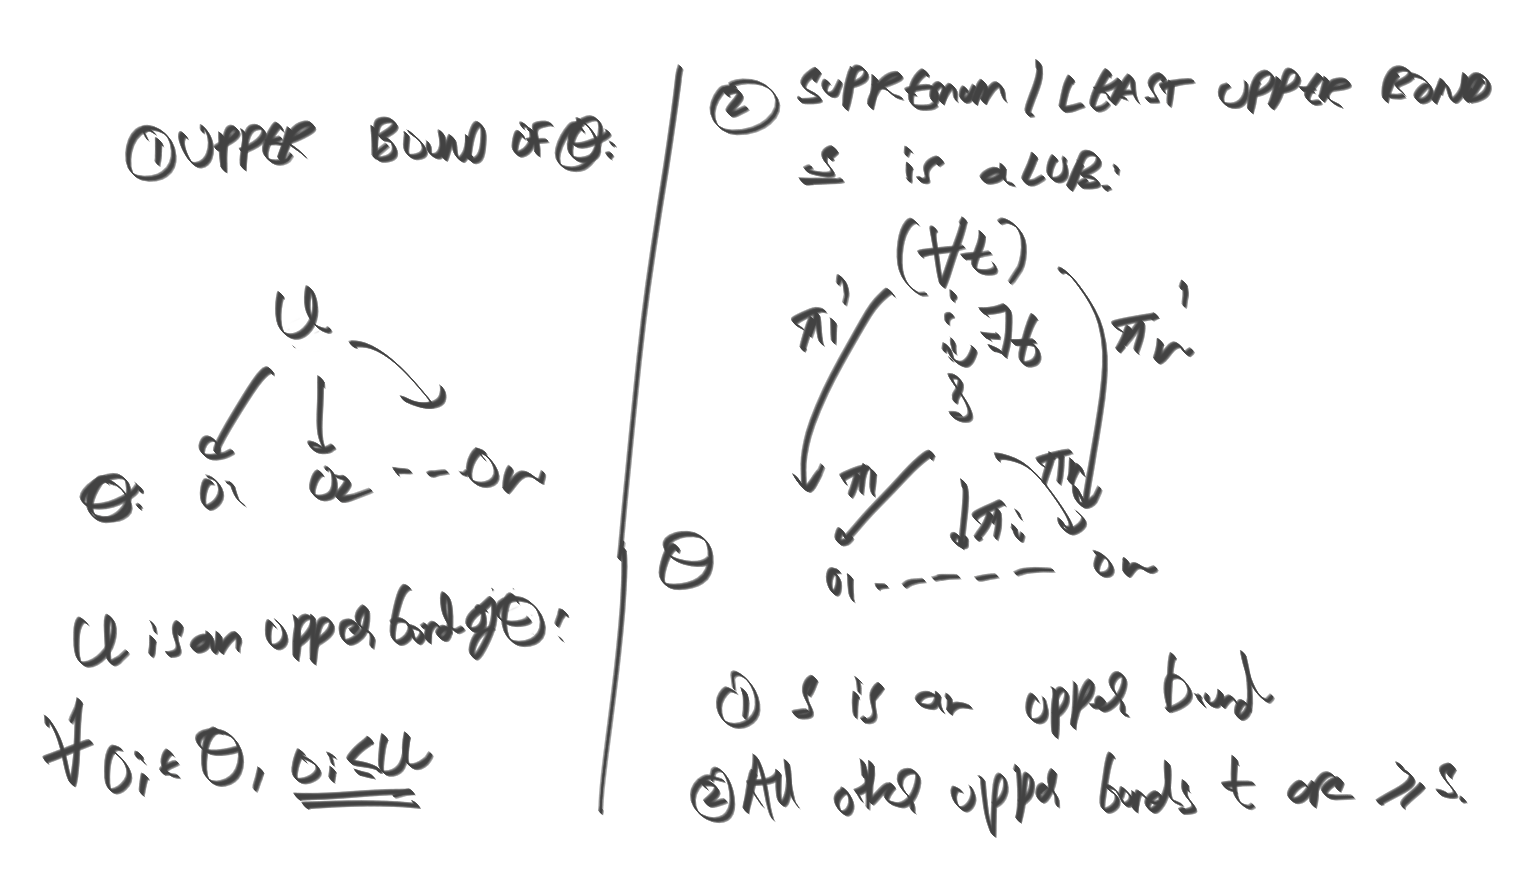
\includegraphics[width=\textwidth]{ch1/sup.png}
    \begin{center}Upper bound and supremum\end{center}
\end{minipage}

\section{Functors}

\question{Exercise 1.3.i}  What is a functor between groups, when regarded as one-object categories?


\proof{} It's going to be a group homomorphism. Since, a functor preserves composition, we have that a
functor $F: C \rightarrow D$ preserves the group structure; for elements of the group / isos $f, g \in Hom(G, G)$, 
we have that the functor obeys $F(f \circ_G g) = (F f) \circ_H (F g)$, which is exactly the equation
we need to preserve group structure. For example, since a functor preserves isomorphisms, an element of the group $f \in Hom(G, G)$
is mapped to an inverbile element $F(f) \in Hom(H, H)$. \qed


\question{Exercise 1.3.ii}  What is a functor between preorders, regarded as a category?

\proof{}Going to be a preorder morphism. I don't know what these are called; If we had a partial order, these
would be called monotone maps. Recall that $a \rightarrow b$ is the encoding of $a \leq b$  within the category.
Suppose we have a functors between preorders (encoded as categories) $F: C \rightarrow D$. Since $F$ preserves
identity arrows, and $a \leq a$ is encoded as $id_a$, we have that $F(a) \leq F(a)$ as:

$$F(a \leq a) = F(id_a) = id_{F(a)} = F(a) \leq F(a)$$


Similarly, since functors take arrows to arrows, the fact that $a \leq b$ which is witnessed by an arrow $a \xrightarrow{f} b$
translates to an arrow $F(a) \xrightarrow{F f} F(b)$, which stands for the relation $F(a) \leq F(b)$. Thus, the map indeed
preserves the preorder structure. Preservation of composition of arrows preserves transitivity of the order relation. \qed


\question{Exercise 1.3.iii} Objects and morphisms in the image of a functor $F: C \rightarrow D$ do not necessarily define a subcategory of $D$.

\proof{} Recall that a morphism can \emph{smoosh} objects, thereby creating coalescing the domains and codomains
of arrows that used to be disjoint. Concretely, consider the diagram:

% https://q.uiver.app/?q=WzAsMTAsWzAsMCwiYSJdLFsxLDAsImIiXSxbMCwxLCJjIl0sWzEsMSwiZCJdLFszLDAsIngiXSxbMywxLCJ6Il0sWzQsMCwieSJdLFszLDIsIng6YSJdLFs0LDIsInk6YixjIl0sWzMsMywiejpkIl0sWzAsMSwiZiJdLFsyLDMsImciXSxbNCw1LCJnIFxcY2lyYyBmIiwyXSxbNiw1LCJsIl0sWzcsOCwiazpmIl0sWzcsOSwiZyBcXGNpcmMgZiIsMl0sWzgsOSwibDpnIl0sWzQsNiwiayJdXQ==
% https://q.uiver.app/?q=WzAsNCxbMCwwLCJhIl0sWzEsMCwiYiJdLFswLDEsImMiXSxbMSwxLCJkIl0sWzIsMywiZyJdLFswLDEsImYiXV0=
\[\begin{tikzcd}
	a & b \\
	c & d
	\arrow["g", from=2-1, to=2-2]
	\arrow["f", from=1-1, to=1-2]
\end{tikzcd}\]

Where we have a category of four objects $a, b, c, d$ with two disconnected arrow $f: a \to b$, and $g: c \to d$.
This is the domain of the functor we will build. The codomain is a three object category:

% https://q.uiver.app/?q=WzAsMyxbMCwwLCJ4Il0sWzEsMCwieSJdLFswLDEsInoiXSxbMCwxLCJrIl0sWzEsMiwibCJdLFswLDIsImxcXGNpcmMgayIsMl1d
\[\begin{tikzcd}
	x & y \\
	z
	\arrow["k", from=1-1, to=1-2]
	\arrow["l", from=1-2, to=2-1]
	\arrow["{l\circ k}"', from=1-1, to=2-1]
\end{tikzcd}\]


The functor will smoosh the four objects into three with a functor, which sends $a$ to $x$, both $b, c$ to $y$, and $d$ to $z$.
Now the image of the functor only has the arrows $k, l$, but not the composite $l \circ k$, which makes the image NOT a subcategory.

% https://q.uiver.app/?q=WzAsMyxbMCwwLCJ4OmEiXSxbMSwwLCJ5OmIsYyJdLFswLDEsIno6ZCJdLFswLDEsIms6ZiJdLFsxLDIsImw6ZyJdLFswLDIsImxcXGNpcmMgazogXFxfIiwyXV0=
\[\begin{tikzcd}
	{x:a} & {y:b,c} \\
	{z:d}
	\arrow["{k:f}", from=1-1, to=1-2]
	\arrow["{l:g}", from=1-2, to=2-1]
	\arrow["{l\circ k: \_}"', from=1-1, to=2-1]
\end{tikzcd}\]



\question{Exercise 1.3.iv} Very that the Hom-set construction is functorial.


\question{Exercise 1.3.v} What is the difference between a functor $F: C^\op \rightarrow D$ and a functor $F: C \rightarrow D^\op$?

\proof{} There is no difference. The functor $C^\op \rightarrow D$ looks like:
% https://q.uiver.app/?q=WzAsNixbMSwwLCJiIl0sWzEsMSwiYSJdLFsyLDAsIkZhIl0sWzIsMSwiRmIiXSxbMCwwLCJhIl0sWzAsMSwiYiJdLFswLDJdLFsxLDNdLFswLDEsImZfe29wfSIsMCx7InN0eWxlIjp7ImJvZHkiOnsibmFtZSI6InNxdWlnZ2x5In19fV0sWzIsMywiRmZfe29wfSJdLFs0LDUsImYiLDJdXQ==
\[\begin{tikzcd}
	a & b & Fa \\
	b & a & Fb
	\arrow[from=1-2, to=1-3]
	\arrow[from=2-2, to=2-3]
	\arrow["{f_{op}}", squiggly, from=1-2, to=2-2]
	\arrow["{Ff_{op}}", from=1-3, to=2-3]
	\arrow["f"', from=1-1, to=2-1]
\end{tikzcd}\]

while the functor $G: D \rightarrow C^{op}$ looks like:

% https://q.uiver.app/?q=WzAsNixbMCwwLCJwIl0sWzAsMSwicSJdLFsxLDAsIkdwIl0sWzEsMSwiR3EiXSxbMiwwLCJHcCJdLFsyLDEsIkdxIl0sWzAsMSwiZiJdLFswLDJdLFsyLDMsIkdmIiwyLHsic3R5bGUiOnsiYm9keSI6eyJuYW1lIjoic3F1aWdnbHkifX19XSxbMSwzXSxbNSw0LCJHZiIsMl1d
\[\begin{tikzcd}
	p & Gp & Gp \\
	q & Gq & Gq
	\arrow["f", from=1-1, to=2-1]
	\arrow[from=1-1, to=1-2]
	\arrow["Gf"', squiggly, from=1-2, to=2-2]
	\arrow[from=2-1, to=2-2]
	\arrow["Gf"', from=2-3, to=1-3]
\end{tikzcd}\]

Given a functor $F: C^{op} \rightarrow D$, we can build an associated functor $G_F: C \rightarrow D^{op}$. Consider
an arrow $x \rightarrow{f} y \in C$ . Dualize it, giving us an arrow $y_{op} \xrightarrow{f_{op}} x_{op} \in C^{op}$. Find
it image under $F$, which gives us an arrow $F(y_{op}) \xrightarrow{F(f_{op})} F(x_{op}) \in D$. Dualize this
in $D$, giving us $F(x_{op})_{op} \xrightarrow{F(f_{op})}_{op} F(y_{op}) \in D^{op}$. See that the arrow
direction coincides with the domain arrow direction $x \rightarrow{f} y \in C$. So we can build a functor $H$
which sends the arrow $x \rightarrow{f} y \in C$ to the arrow $F(x_{op})_{op} \xrightarrow{F(f_{op})}_{op} F(y_{op}) \in D^{op}$.
Hence, $H: C \rightarrow D^{op}$, defined by $H(x) \equiv F(x_{op})_{op}$ and $H(f) \equiv F(f_{op})_{op}$. 
By duality, we get the other direction where we start from $F': C \rightarrow D^{op}$ and end at $H': C^{op} \rightarrow D$.
Thus, the two are equivalent.

In a nutshell, the diagram is:

% https://q.uiver.app/?q=WzAsMTUsWzEsMCwiYiJdLFsxLDEsImEiXSxbMiwwLCJGYiJdLFsyLDEsIkZhIl0sWzAsMCwiYSJdLFswLDEsImIiXSxbNCwwLCJhIl0sWzQsMSwiYiJdLFs1LDAsIkZhIl0sWzUsMSwiRmIiXSxbNywwLCJGYiJdLFs3LDEsIkZhIl0sWzMsMCwiXFxpbXBsaWVzIl0sWzMsMSwiXFxpbXBsaWVzIl0sWzYsMF0sWzAsMl0sWzEsM10sWzAsMSwiZl97b3B9IiwwLHsic3R5bGUiOnsiYm9keSI6eyJuYW1lIjoic3F1aWdnbHkifX19XSxbMiwzLCJGZl97b3B9Il0sWzQsNSwiZiIsMl0sWzYsNywiZiJdLFs2LDhdLFs4LDksIihGZilfe29wfSIsMCx7InN0eWxlIjp7ImJvZHkiOnsibmFtZSI6InNxdWlnZ2x5In19fV0sWzcsOV0sWzEwLDExLCJGZl97b3B9Il1d
\[\begin{tikzcd}
	a & b & Fb & \implies & a & Fa & {} & Fb \\
	b & a & Fa & \implies & b & Fb && Fa
	\arrow[from=1-2, to=1-3]
	\arrow[from=2-2, to=2-3]
	\arrow["{f_{op}}", squiggly, from=1-2, to=2-2]
	\arrow["{Ff_{op}}", from=1-3, to=2-3]
	\arrow["f"', from=1-1, to=2-1]
	\arrow["f", from=1-5, to=2-5]
	\arrow[from=1-5, to=1-6]
	\arrow["{(Ff)_{op}}", squiggly, from=1-6, to=2-6]
	\arrow[from=2-5, to=2-6]
	\arrow["{Ff_{op}}", from=1-8, to=2-8]
\end{tikzcd}\]



\question{Exercise 1.3.vi} Given the comma category $F \downarrow G$, define the domain and codomain projection functors $dom: F \comma G \rightarrow F$
  and $codom: F \comma G \rightarrow G$.


Recall that an object in the comma category is a a triple $(d \in D, e \in E, F(d) \xrightarrow{f} F(e))$, or diagramatically:

% https://q.uiver.app/?q=WzAsNCxbMCwwLCJkIFxcaW4gRCJdLFsxLDAsImUgXFxpbiBFIl0sWzAsMSwiRmRcXGluIEMiXSxbMSwxLCJHZSBcXGluIEMiXSxbMCwyLCJGOiBEICIsMl0sWzEsMywiRyJdLFsyLDMsImYiLDJdXQ==
\[\begin{tikzcd}
	{d \in D} & {e \in E} \\
	{Fd\in C} & {Ge \in C}
	\arrow["{F: D }"', from=1-1, to=2-1]
	\arrow["G", from=1-2, to=2-2]
	\arrow["f"', from=2-1, to=2-2]
\end{tikzcd}\]

and a morphism in such a category is a diagram:

% https://q.uiver.app/?q=WzAsNyxbMSwwLCJGZCJdLFsyLDAsIkdlIl0sWzEsMiwiRmQnIl0sWzIsMiwiR2UnIl0sWzAsMiwiKGQnLCBlJyxmJykiXSxbNSwyXSxbMCwwLCIoZCwgZSxmKSJdLFsyLDMsImYnIiwyXSxbMCwxLCJmIiwyXSxbMCwyLCJcXGFscGhhIiwxXSxbMSwzLCJcXGJldGEgIiwxXSxbNiw0LCIoXFxhbHBoYSBcXGRvd25hcnJvdyBcXGJldGEpIiwxXV0=
\[\begin{tikzcd}
	{(d, e,f)} & Fd & Ge \\
	\\
	{(d', e',f')} & {Fd'} & {Ge'} &&& {}
	\arrow["{f'}"', from=3-2, to=3-3]
	\arrow["f"', from=1-2, to=1-3]
	\arrow["\alpha"{description}, from=1-2, to=3-2]
	\arrow["{\beta }"{description}, from=1-3, to=3-3]
	\arrow["{(\alpha \downarrow \beta)}"{description}, from=1-1, to=3-1]
\end{tikzcd}\]

We constrct the domain functor $dom$ as a functor that sends an object $(d \in D, e \in E, F(d) \xrightarrow{f} F(e))$ to an object $d \in D$.
It sends the morphism between $(d, e, f)$ and $(d', e', f')$, given by $(\alpha : Fd \rightarrow Fd', \beta: Ge \rightarrow Ge')$ to
the arrow $Fd \xrightarrow{\alpha} Fd' \in D$.

In a diagram, this looks like:

% https://q.uiver.app/?q=WzAsMTAsWzEsMCwiRmQiXSxbMiwwLCJHZSJdLFsxLDIsIkZkJyJdLFsyLDIsIkdlJyJdLFswLDAsIihkLCBlLGYpIl0sWzAsMiwiKGQnLCBlJyxmJykiXSxbNSwyXSxbMywxLCJcXHhyaWdodGFycm93e2RvbX0iXSxbNCwwLCJGZCJdLFs0LDIsIkZkJyJdLFsyLDMsImYnIiwyXSxbMCwxLCJmIiwyXSxbMCwyLCJcXGFscGhhIiwxXSxbMSwzLCJcXGJldGEgIiwxXSxbNCw1LCIoXFxhbHBoYSBcXGRvd25hcnJvdyBcXGJldGEpIiwxXSxbOCw5LCJcXGFscGhhIiwxXV0=
\[\begin{tikzcd}
	{(d, e,f)} & Fd & Ge && Fd \\
	&&& {\xrightarrow{dom}} \\
	{(d', e',f')} & {Fd'} & {Ge'} && {Fd'} & {}
	\arrow["{f'}"', from=3-2, to=3-3]
	\arrow["f"', from=1-2, to=1-3]
	\arrow["\alpha"{description}, from=1-2, to=3-2]
	\arrow["{\beta }"{description}, from=1-3, to=3-3]
	\arrow["{(\alpha \downarrow \beta)}"{description}, from=1-1, to=3-1]
	\arrow["\alpha"{description}, from=1-5, to=3-5]
\end{tikzcd}\]

$codom$ will do the same thing, by stripping out the codomain of the comma instead of the domain. \qed

\question{Exercise 1.3.vii} Define slice category as special case of the comma category.


\proof{} To define the slice $C/c$ whose objects are of the form $d \rightarrow c$ for varying $d \in C$, we pick
the category $D = C, E = C$, and functors $F : C \rightarrow C = id$, $G : C \rightarrow C = \delta_c$, that is, the constant functor
which smooshes the entire $C$ category into the object $c \in C$ by mapping all objects to $c$ and all arrows to $id_{c}$.

This causes the diagram to collapse down to objects of the form $d \rightarrow c$, and the arrows to be what we'd expect \qed.

\question{Exercise 1.3.viii} Show that functors need not reflect isomorphisms. for a functor $F: C \rightarrow D$, and a 
morphisms $f \in C$ such that $F f$ is an isomorphism in $D$ but $f$ is not an isomorphism in $C$.


Pick a category $C$ and an object $o \in C$. Build the constant functor $\delta_o: C \rightarrow C$. The image
of every arrow $c \xrightarrow{a} c'$ is the identity arrow $id_o$ which is an iso. The arrow $a$ need not be iso. The functor
$\delta_o$ does not reflect isos. \qed

\question{Exercise 1.3.ix} Consider the not-yet-functors $Grp \rightarrow Grp$ that sends a group to its center, comutator subgroup, and automorphism group.
Are these functors if we limit the category $Grp$ to have (a) only isomorphisms? (b) only epimorphisms? (c) all homomorphisms?

\proof[(isos)] If we have (a) only isomorphisms, then these are indeed functors, since an isomorphism $G \simeq H$
implies that their group theoretic properties are identical. Thus, we will have
$Z(G) \simeq Z(H)$, ie, isomorphic centers.
Thus, an iso arrow $f: G \rightarrow H$ becomes an iso arrow
$Z(f) : Z(G) \rightarrow Z(H)$. The exact same happens for commutator and automorphism. \qed

\proof[(epis)] If we only have epimorphisms, we first invoke  given footnote 29, that all
epis in Group are surjections. Thus, given an epi (surjection) $\phi: G \twoheadrightarrow H$, we
identify $im(\phi) \simeq G/ker(\phi)$ or $H \simeq G/ker(\phi)$, since $H \simeq im(\phi)$ by $\phi$ being a surjection.
So we can choose to study only quotient maps $\phi: G \rightarrow G/ker \phi$.

For the center, consider the determinant map $|\cdot|: GL(2, \mathbb R) \rightarrow \mathbb R^\times$.
This map is surjective since we can pick the matrix $\begin{bmatrix} 1 & 0 \\ 0 & r \end{bmatrix}$ to get all possible
determinants  for arbitrary $r \in \mathbb R$. The center
of the group of matrices is scalar multiples of the identity, thus $Z(GL(2, \mathbb R)) = \{ k I : k \in \mathbb R \}$.
The center of the reals $Z(\mathbb R^\times)$ is the reals themselves since it's an abelian group. Now see
that the determinant of a matrix $kI$ must be $k^2$, since we get two copies of $k$ along the diagonal. Thus, the image
$\phi(Z(GL(2, \mathbb R))) = \{ k^2 : k \in \mathbb R \} = \mathbb R_{\geq 0}$ which is smaller than the center of the image,
$Z(\phi(GL(2, \mathbb R))) = Z(\mathbb R^{\times}) = \mathbb R^\times$. Thus, \textbf{the center not functorial on epis}.

\section{Natural Transformations}

\subsection{Musing}
\subsubsection{Torsion decomposition}

Let $TA$ be the subgroup of $A$ that have finite order.

\begin{itemize}
\item The idea is to first show that any natural transformation of the identity functor $\eta: 1 \implies 1$ is multiplication by some $n \in \Z$
(recall that every abelian group is a \Z-module, so this is a sensible thing to say).
\item Let's study the component of $\eta$ at $\mathbb Z$.
This means that we have an arrow at $1(\Z) \xrightarrow{\eta(id)} 1(\Z)$, which is $\Z \rightarrow{\eta(id)} \Z$ since identity functor
leaves objects and arrow invariant. Any arrow $\Z \xrightarrow{\eta(id)} \Z$ is a multiplication by some natural number.
\item Now consider a homomorphism $f: \Z \rightarrow A$. This is determined entirely by $f(1) \in A$, so any such map is 
  the same as picking an element $a \in A$. 
\item Let's now consider the isomorphism $A \epi A/TA \mono TA \oplus (A/TA) \simeq A$. If this isomorphism were natural,
    then we would have a natural endomorphism of the identity functor $\alpha: 1 \rightarrow 1$.
\item Let's observe $\alpha$ at $\mathbb Z$. We already know that such a transformation is given by $\Z \xrightarrow{\alpha} \Z$,
    which is multiplication b a number $n \neq 0$ (can't be zero since we need an isomorphism).
\item Now consider $C \equiv \Z/2n\Z$ where $n$ is the $\alpha$ scale factor. See that $T(\Z/2n\Z) = \Z/2n\Z$.
    So we get the factoring as $\Z/2n\Z \epi 0 \mono \Z/2n\Z \oplus 0 \simeq \Z/2n\Z$. Since we factor through zero,
    the full map is the zero map. However, we know from the natural transformation that the natural transformation 
    must scale all elements by $n \neq 0$. So we break naturality
\end{itemize}

The big thing I don't understand in this is why we need to factor \emph{through} the epi. If I directly define
$A \rightarrow (A/TA) \oplus TA$, given by the exact sequence $0 \mono TA \mono A \epi A/TA \epi 0$? Ah I see, this sequence
need not always split. 

\subsubsection{Walking arrow for unnatural isomorphism}

Consider the category $I \equiv (0 \rightarrow 1)$. Consider functors $F: I \rightarrow Vec(\R)$. The functor
picks out morphsisms between real vector spaces. If we consider endomorphisms, I could consider a functor $F_{id}$ that picked
out the identity map from $\R$ to $\R$, and another $F_{0}$ that picked out the constant linear function $f(x) = 0$ from $\R$ to $\R$.
These have the same domain and range, but the actual action of the arrow is wildly different. So, for a natural transformation
to be natural, it's not enough to have the same action on objects (clearly!)


\subsubsection{Permutations and total orderings for unnatural isomorphism}

Consider a subcategory of $Set$ containing only bijections.  Define the functor
$Perm: Set \rightarrow Set$ which takes a set $S$ to its set of permutations, where a permutation
is a bijection $S \rightarrow S$, and the functor $Ord: Set \rightarrow Set$ which takes a set $S$ to its total orderings, where a total ordering
is a bijection $\{1, 2, \dots |S|\} \rightarrow S$. We claim that there is no natural transformation between these two functors.
To see why, let us study the situation on the smallest non-trivial case, a two element set $\{a, b\}$.

With the chosen arrow as $id: [a \mapsto a; b \mapsto b]$, we get the commutative diagram for the naturality square as:

% https://q.uiver.app/?q=WzAsOCxbMCwxLCJbYSBcXG1hcHN0byBhOyBiIFxcbWFwc3RvIGJdIFthIFxcbWFwc3RvIGI7IGIgXFxtYXBzdG8gYV0iXSxbMCw0LCJbMSBcXG1hcHN0byBhOyAyIFxcbWFwc3RvIGJdWzEgXFxtYXBzdG8gYjsgMlxcbWFwc3RvIGFdIl0sWzUsMSwiW2EgXFxtYXBzdG8gYTsgYiBcXG1hcHN0byBiXSBbYSBcXG1hcHN0byBiOyBiIFxcbWFwc3RvIGFdIl0sWzAsMCwiaWRfQSBcXGVxdWl2W2EgXFxtYXBzdG8gYTsgYlxcbWFwc3RvIGJdIl0sWzUsNCwiWzEgXFxtYXBzdG8gYTsgMiBcXG1hcHN0byBiXVsxIFxcbWFwc3RvIGI7IDIgXFxtYXBzdG8gYV0iXSxbNSwzLCJbMVxcbWFwc3RvIGE7IDJcXG1hcHN0byBiXVsxIFxcbWFwc3RvIGI7IDIgXFxtYXBzdG8gYV0iXSxbMyw0XSxbNCw0XSxbMCwxLCJcXGV0YV9BIl0sWzIsNSwiXFxldGFfQSIsMl0sWzEsNCwiT3JkKGlkX0EpKGYpID1pZF9BIFxcY2lyYyBmID0gZiJdLFswLDIsIlBlcm0oaWRfQSkoZik9aWRfQSBcXGNpcmMgZiBcXGNpcmMgaWRfQV57LTF9ID0gZiIsMl0sWzUsNCwiXFx0ZXh0e2VxdWFsfSIsMl1d
\[\begin{tikzcd}
	{id_A \equiv[a \mapsto a; b\mapsto b]} \\
	{[a \mapsto a; b \mapsto b] [a \mapsto b; b \mapsto a]} &&&&& {[a \mapsto a; b \mapsto b] [a \mapsto b; b \mapsto a]} \\
	\\
	&&&&& {[1\mapsto a; 2\mapsto b][1 \mapsto b; 2 \mapsto a]} \\
	{[1 \mapsto a; 2 \mapsto b][1 \mapsto b; 2\mapsto a]} &&& {} & {} & {[1 \mapsto a; 2 \mapsto b][1 \mapsto b; 2 \mapsto a]}
	\arrow["{\eta_A}", from=2-1, to=5-1]
	\arrow["{\eta_A}"', from=2-6, to=4-6]
	\arrow["{Ord(id_A)(f) =id_A \circ f = f}", from=5-1, to=5-6]
	\arrow["{Perm(id_A)(f)=id_A \circ f \circ id_A^{-1} = f}"', from=2-1, to=2-6]
	\arrow["{\text{equal}}"', from=4-6, to=5-6]
\end{tikzcd}\]

While with the chosen arrow as $\sigma: [a \mapsto b; b \mapsto a]$ we get the non-commuting diagram for the naturality square as:

% https://q.uiver.app/?q=WzAsNixbMCwxLCJbYSBcXG1hcHN0byBhOyBiIFxcbWFwc3RvIGJdIFthIFxcbWFwc3RvIGI7IGIgXFxtYXBzdG8gYV0iXSxbMCw0LCJbMSBcXG1hcHN0byBhOyAyIFxcbWFwc3RvIGJdWzEgXFxtYXBzdG8gYjsgMlxcbWFwc3RvIGFdIl0sWzYsMSwiW2IgXFxtYXBzdG8gYjsgYSBcXG1hcHN0byBhXSBbYiBcXG1hcHN0byBhOyBhIFxcbWFwc3RvIGJdIl0sWzAsMCwiXFxzaWdtYSBcXGVxdWl2W2EgXFxtYXBzdG8gYjsgYlxcbWFwc3RvIGFdIl0sWzYsNCwiWzEgXFxtYXBzdG8gYjsgMiBcXG1hcHN0byBhXVsxIFxcbWFwc3RvIGE7IDIgXFxtYXBzdG8gYl0iXSxbNiwzLCJbMlxcbWFwc3RvIGI7IDEgXFxtYXBzdG8gYV1bMiBcXG1hcHN0byBhOyAxIFxcbWFwc3RvIGJdIl0sWzAsMSwiXFxldGFfQSJdLFswLDIsIlBlcm0oXFxzaWdtYSkoZikgPSBcXHNpZ21hIFxcY2lyYyBmIFxcY2lyYyBcXHNpZ21hXnstMX0iLDJdLFsxLDQsIk9yZChcXHNpZ21hKShmKSA9IFxcc2lnbWEgXFxjaXJjIGYiXSxbMiw1LCJcXGV0YV9BIiwyXSxbNSw0LCJcXHRleHR7bm90IGVxdWFsfSIsMix7InN0eWxlIjp7ImhlYWQiOnsibmFtZSI6Im5vbmUifX19XV0=
\[\begin{tikzcd}
	{\sigma \equiv[a \mapsto b; b\mapsto a]} \\
	{[a \mapsto a; b \mapsto b] [a \mapsto b; b \mapsto a]} &&&&&& {[b \mapsto b; a \mapsto a] [b \mapsto a; a \mapsto b]} \\
	\\
	&&&&&& {[2\mapsto b; 1 \mapsto a][2 \mapsto a; 1 \mapsto b]} \\
	{[1 \mapsto a; 2 \mapsto b][1 \mapsto b; 2\mapsto a]} &&&&&& {[1 \mapsto b; 2 \mapsto a][1 \mapsto a; 2 \mapsto b]}
	\arrow["{\eta_A}", from=2-1, to=5-1]
	\arrow["{Perm(\sigma)(f) = \sigma \circ f \circ \sigma^{-1}}"', from=2-1, to=2-7]
	\arrow["{Ord(\sigma)(f) = \sigma \circ f}", from=5-1, to=5-7]
	\arrow["{\eta_A}"', from=2-7, to=4-7]
	\arrow["{\text{not equal}}"', no head, from=4-7, to=5-7]
\end{tikzcd}\]

We see that we cannot define a single $\eta_A$ that works in both cases.

\subsubsection{Group as category v/s poset category}

in poset as category, objects carry most of the structure, not many arrows. In
group as category, only one object, many arrows.

\subsection{Exercises}

\question{Exercise 1.4.i} Let $\alpha: F \nt G$ be a natural isomorphism. Show that the inverses of the components define a natural isomorphism $\inv\alpha: G \nt F$.

We need to show that the square with $?$ in it commutes, given the square on top:

% https://q.uiver.app/?q=WzAsMTMsWzEsMCwiRngiXSxbMiwwLCJHeCJdLFsxLDEsIkZ5Il0sWzIsMSwiR3kiXSxbMCwwLCJ4Il0sWzAsMSwieSJdLFsyLDJdLFsxLDIsIkd4Il0sWzMsMiwiRngiXSxbMSw0LCJHeSJdLFszLDQsIkZ5Il0sWzIsMywiPyJdLFszLDNdLFswLDEsIlxcZXRhKHgpIl0sWzAsMiwiRmEiLDJdLFsyLDMsIlxcZXRhKHkpIiwyXSxbMSwzLCJHYSJdLFs0LDUsImEiLDJdLFs3LDksIkdhIiwyXSxbOCwxMCwiRmEiXSxbNyw4LCJcXGV0YV57LTF9KHgpIl0sWzksMTAsIlxcZXRhXnstMX0oeSkiLDJdXQ==
\[\begin{tikzcd}
	x & Fx & Gx \\
	y & Fy & Gy \\
	& Gx & {} & Fx \\
	&& {?} & {} \\
	& Gy && Fy
	\arrow["{\eta(x)}", from=1-2, to=1-3]
	\arrow["Fa"', from=1-2, to=2-2]
	\arrow["{\eta(y)}"', from=2-2, to=2-3]
	\arrow["Ga", from=1-3, to=2-3]
	\arrow["a"', from=1-1, to=2-1]
	\arrow["Ga"', from=3-2, to=5-2]
	\arrow["Fa", from=3-4, to=5-4]
	\arrow["{\eta^{-1}(x)}", from=3-2, to=3-4]
	\arrow["{\eta^{-1}(y)}"', from=5-2, to=5-4]
\end{tikzcd}\]

From the square, we know that $Ga \circ \eta(x) = \eta(y) \circ Fa$. Using inverses, we derive:

\begin{align*}
&Ga \circ \eta(x) = \eta(y) \circ Fa \\
&Ga \circ \eta(x) \circ \eta^{-1}(x) = \eta(y) \circ Fa \circ \eta^{-1}(x) \\
&Ga \circ id_x = \eta(y) \circ Fa \circ \eta^{-1}(x) \\
&Ga = \eta(y) \circ Fa \circ \eta^{-1}(x) \\
&\eta^{-1}(y) \circ Ga = \eta^{-1}(y) \circ \eta(y) \circ Fa \circ \eta^{-1}(x) \\
&\eta^{-1}(y) \circ Ga = id_y \circ Fa \circ \eta^{-1}(x) \\
&\eta^{-1}(y) \circ Ga = Fa \circ \eta^{-1}(x) \\
\end{align*}

which is exactly the diagram:

% https://q.uiver.app/?q=WzAsOSxbMywwXSxbMiwwLCJHeCJdLFs0LDAsIkZ4Il0sWzIsMiwiR3kiXSxbNCwyLCJGeSJdLFszLDEsIlxcZXRhXnstMX0oeSkgXFxjaXJjIEdhID0gRmEgXFxjaXJjIFxcZXRhXnstMX0oeCkiXSxbNCwxXSxbMCwwLCJ4Il0sWzAsMiwieSJdLFsxLDMsIkdhIiwyXSxbMiw0LCJGYSJdLFsxLDIsIlxcZXRhXnstMX0oeCkiXSxbMyw0LCJcXGV0YV57LTF9KHkpIiwyXSxbNyw4LCJhIiwyXV0=
\[\begin{tikzcd}
	x && Gx & {} & Fx \\
	&&& {\eta^{-1}(y) \circ Ga = Fa \circ \eta^{-1}(x)} & {} \\
	y && Gy && Fy
	\arrow["Ga"', from=1-3, to=3-3]
	\arrow["Fa", from=1-5, to=3-5]
	\arrow["{\eta^{-1}(x)}", from=1-3, to=1-5]
	\arrow["{\eta^{-1}(y)}"', from=3-3, to=3-5]
	\arrow["a"', from=1-1, to=3-1]
\end{tikzcd}\]


\question{Exercise 1.4.ii} What is a natural transformation between a parallel pair of functors between groups regarded as one object categories?

\proof{} Let $G, H$ be groups regarded as one object categories, so elements are arrows. A functor $F: G \rightarrow H$ is a group homomorphism. Two functors $F, F': G \rightarrow H$
are two group homomorphisms. An natural transformation is a map $\eta: G \rightarrow H$ which for every (the only) object $*_G \in G$, assigns
an arrow $\eta(*_G): F(*_G) \xrightarrow{\eta(*_G)} G(*_G)$ which is compatible with all arrows:

% https://q.uiver.app/?q=WzAsNSxbMCwwLCJGKCopIFxcaW4gSCJdLFsxLDAsIkYnKCopIFxcaW4gSCJdLFswLDEsIkYoKikgXFxpbiBIIl0sWzEsMSwiRicoKikgXFxpbiBIIl0sWzEsMl0sWzAsMSwiXFxldGEoKikiXSxbMiwzLCJcXGV0YSgqKSJdLFswLDIsIkYoaCkiLDFdLFsxLDMsIkYnKGgpIiwxXV0=
\[\begin{tikzcd}
	{F(*_G) \in H} & {F'(*_G) \in H} \\
	{F(*_G) \in H} & {F'(*_G) \in H} \\
	& {}
	\arrow["{\eta(*_G)}", from=1-1, to=1-2]
	\arrow["{\eta(*_G)}", from=2-1, to=2-2]
	\arrow["{F(g)}"{description}, from=1-1, to=2-1]
	\arrow["{F'(g)}"{description}, from=1-2, to=2-2]
\end{tikzcd}\]

Simplifying the diagram by substituting $F(*) = F'(*) = *$, and setting $\alpha \equiv \eta(*G) \in Hom(*_H, *_H)$, we get:

% https://q.uiver.app/?q=WzAsNSxbMCwwLCIqX0giXSxbMSwwLCIqX0giXSxbMCwxLCIqX0giXSxbMSwxLCIqX0giXSxbMSwyXSxbMCwxLCJcXGFscGhhIFxcZXF1aXYgXFxldGEoKl9HKSJdLFsyLDMsIlxcYWxwaGEgXFxlcXVpdiBcXGV0YSgqX0cpIiwyXSxbMSwzLCJGJyhoKSJdLFswLDIsIkYoaCkiLDJdXQ==
\[\begin{tikzcd}
	{*_H} & {*_H} \\
	{*_H} & {*_H} \\
	& {}
	\arrow["{\alpha \equiv \eta(*_G)}", from=1-1, to=1-2]
	\arrow["{\alpha \equiv \eta(*_G)}"', from=2-1, to=2-2]
	\arrow["{F'(g)}", from=1-2, to=2-2]
	\arrow["{F(g)}"', from=1-1, to=2-1]
\end{tikzcd}\]

So we are looking for an arrow (group element) $\alpha \in H$ such that for all $g \in G$, $F'(g) \cdot \alpha = \alpha \cdot F(g)$.
On rearranging: $\alpha^{-1} \cdot F'(g) \cdot \alpha = F(g)$. So it gives a sort of  ``inner automorphism'' from $F$ to $F'$. \qed


\question{Exercise 1.4.iii} What is a natural transformation between a parallel pair of functors between preorders regarded as categories?
\proof{} We regard preorders as thin categories, where there is an most arrow from $p \rightarrow p'$ if $p \leq p'$. A functor from $(P, \leq)$ to $(Q, \leq)$
is a monotone map. A pair of functors $F, G: P \rightarrow Q $ is a pair of monotone maps. A natural transformation $\eta: F \nt G$ makes for each $p \in $P
the diagram commute:

% https://q.uiver.app/?q=WzAsNixbMiwwLCJGKHApIl0sWzMsMCwiRyhwKSJdLFsyLDEsIkYocSkiXSxbMywxLCJHKHEpIl0sWzAsMCwicCJdLFswLDEsInEiXSxbMCwxLCJcXGV0YShwKSJdLFsyLDMsIlxcZXRhKHEpIl0sWzAsMiwiRihwPHEpIiwyXSxbMSwzLCJHKHAgPCBxKSJdLFs0LDUsInA8IHEiXV0=
\[\begin{tikzcd}
	p && {F(p)} & {G(p)} \\
	p' && {F(p')} & {G(p')}
	\arrow["{\eta(p)}", from=1-3, to=1-4]
	\arrow["{\eta(p)}", from=2-3, to=2-4]
	\arrow["{F(p<p')}"', from=1-3, to=2-3]
	\arrow["{G(p < p')}", from=1-4, to=2-4]
	\arrow["{p< p'}", from=1-1, to=2-1]
\end{tikzcd}\]

So, for every $p \leq p'$, the functor $F$ maps us to elements $F(p) \leq F(p')$, and $G$ maps us to elements $G(p) \leq G(p')$. The natural transformation $\eta$
asks to witness an arrow $F(p) \xrightarrow{\eta(p)} G(p)$, which means that we must have $F(p) \leq G(p)$ within the category $Q$, and similarly for $p'$.
Thus, it witnesses that $G$ is always \emph{above} $F$. For any element $p \in P$, we will always have $F(p) \leq G(p)$, in a way that is consistent with the
monotonicity of $F, G$.


\question{Exercise 1.4.iv} Prove that distinct parallel morphisms $f, g: c^\to_\to d$ define distinct natural transformations $f_*, g_*: C(-, c) \nt C(-, d)$ by pre-composition.

Recall that the natural transformation by $f_*$ is given for a fixed $o \xrightarrow{a} o'$ by $Hom(o, c) \xrightarrow{f_* \equiv f \circ - } Hom(o, d)$,
and similarly for $g_*$ by $Hom(o, c) \xrightarrow{g_* \equiv g \circ -} Hom(o, d)$. If we choose $o = c$, then we can consider $Hom(c, c)$.
Let' then see where $id_c \in Hom(c, c)$ gets mapped to:

\begin{align*}
&Hom(o, c) \xrightarrow{f_* \equiv f \circ - } Hom(o, d) \\
&Hom(o=c, c) \xrightarrow{_f* \equiv f \circ - } Hom(o=c, d) \\
&Hom(c, c) \xrightarrow{f_* \equiv f \circ - } Hom(c, d) \\
&id_c \in Hom(c, c) \xrightarrow{f_* \equiv f \circ - } f \circ id_c \in Hom(c, d) \\
&id_c \in Hom(c, c) \xrightarrow{f_* \equiv f \circ - } f \in Hom(c, d) \\
\end{align*}

So we map $id \in Hom(c, c)$ into $f \in Hom(c,d)$ by $f_*$. Since there was nothing special about $f$, we similarly map $id \in Hom(c, c)$
into $g \in Hom(c, d)$ by $g_*$. Since the two morphisms are distinct, we have $f \neq g$. 
Thus, the two distinct parallel morphisms $f, g$. natural transformations $f_*$ and $g_*$ are inequivalent since they have different components
on the element $c$: $f_*(c): Hom(c, c) \rightarrow Hom(c, d)$ is not the same action as $g_*(c): Hom(c, c) \rightarrow Hom(c, d)$, since they
act differently on $id_c \in Hom(c, c)$, as $f_*(c)(id_c) = f \neq g = g_*(c)(id_c)$.


\question{Exercise 1.4.v} Consider the comma cataegory $F \downarrow G$ for $F: D \rightarrow C, G: E \rightarrow C$. Construct a canonical natural transformation
$\alpha: F \circ dom \rightarrow G \circ codom$:

% https://q.uiver.app/?q=WzAsNSxbMCwwLCJGIFxcZG93bmFycm93IEciXSxbMiwwLCJFIl0sWzIsMiwiQyJdLFswLDIsIkQiXSxbMSwxLCJcXG5lYXJyb3dfXFxldGEiXSxbMCwxLCJjb2RvbSIsMl0sWzEsMiwiRyIsMl0sWzIsMywiRiIsMl0sWzMsMCwiZG9tIiwyXV0=
\[\begin{tikzcd}
	{F \downarrow G} && E \\
	& {\nearrow_\eta} \\
	D && C
	\arrow["codom"', from=1-1, to=1-3]
	\arrow["G"', from=1-3, to=3-3]
	\arrow["F"', from=3-3, to=3-1]
	\arrow["dom"', from=3-1, to=1-1]
\end{tikzcd}\]


\proof{}

Recall that elements  $k, k \in F \downarrow G$ and arrows $k \xrightarrow{a} k'$ is given by:

% https://q.uiver.app/?q=WzAsNixbMCwwLCJrXFxlcXVpdihkLGUsRmRcXHhyaWdodGFycm93e2Ffa31HZSkiXSxbMCwxLCJrJ1xcZXF1aXYoZCcsZScsRmQnXFx4cmlnaHRhcnJvd3thX3trJ319R2UnKSJdLFszLDAsIkZkIl0sWzMsMSwiRmQnIl0sWzQsMCwiR2UiXSxbNCwxLCJHZSciXSxbMCwxLCJhXFxlcXVpdihkXFx4cmlnaHRhcnJvd3thX2R9ZCcsZVxceHJpZ2h0YXJyb3d7YV9lfWUnKSJdLFsyLDMsIkYoYV9kKSIsMl0sWzIsNCwiYV9rIl0sWzMsNSwiYV9rJyIsMl0sWzQsNSwiRihhX2UnKSJdXQ==
\[\begin{tikzcd}
	{k\equiv(d,e,Fd\xrightarrow{a_k}Ge)} &&& Fd & Ge \\
	{k'\equiv(d',e',Fd'\xrightarrow{a_{k'}}Ge')} &&& {Fd'} & {Ge'}
	\arrow["{a\equiv(d\xrightarrow{a_d}d',e\xrightarrow{a_e}e')}", from=1-1, to=2-1]
	\arrow["{F(a_d)}"', from=1-4, to=2-4]
	\arrow["{a_k}", from=1-4, to=1-5]
	\arrow["{a_k'}"', from=2-4, to=2-5]
    \arrow["{G(a_e)}", from=1-5, to=2-5]
\end{tikzcd}\]

We need to make this diagram commute for all $k, k' \in F \downarrow G$

% https://q.uiver.app/?q=WzAsMTAsWzAsMCwiRlxcY2lyYyBkb20oaykiXSxbMCwyLCJGIFxcY2lyYyBkb20oaycpIl0sWzIsMCwiRyBcXGNpcmMgY29kb20oaykiXSxbMiwyLCJHIFxcY2lyYyBjb2RvbShrJykiXSxbMywxLCI9Il0sWzQsMCwiZCJdLFs0LDIsImQnIl0sWzYsMCwiZSJdLFs2LDIsImUnIl0sWzIsM10sWzAsMSwiRiBcXGNpcmMgZG9tKGEpIiwyXSxbMCwyLCJcXGV0YShrKSJdLFsyLDMsIkcgXFxjaXJjIGNvZG9tKGspIl0sWzEsMywiXFxldGEoaycpIiwyXSxbNSw2LCJGYV9kIl0sWzUsNywiXFxldGEoaykiLDJdLFs2LDgsIlxcZXRhKGsnKSJdLFs3LDgsIkdhX2UiLDJdXQ==
\[\begin{tikzcd}
	{F\circ dom(k)} && {G \circ codom(k)} && d && e \\
	&&& {=} \\
	{F \circ dom(k')} && {G \circ codom(k')} && {d'} && {e'} \\
	&& {}
	\arrow["{F \circ dom(a)}"', from=1-1, to=3-1]
	\arrow["{\eta(k)}", from=1-1, to=1-3]
	\arrow["{G \circ codom(k)}", from=1-3, to=3-3]
	\arrow["{\eta(k')}"', from=3-1, to=3-3]
	\arrow["{Fa_d}", from=1-5, to=3-5]
	\arrow["{\eta(k)}"', from=1-5, to=1-7]
	\arrow["{\eta(k')}", from=3-5, to=3-7]
	\arrow["{Ga_e}"', from=1-7, to=3-7]
\end{tikzcd}\]

To show the equality between the left square and right square, we simplify using the definitions of $k, k'$:
\begin{itemize}
    \item $k \equiv (d, e, Fd \xrightarrow{a_k} Ge)$, $k' \equiv (d', e' Fd' \xrightarrow{a_k'} Ge')$.
    \item $a : k \rightarrow k'$ is given by $a \equiv (d \xrightarrow{a_d} d', e \xrightarrow{a_e} e')$ such that the diagram commutes.
    \item $dom(a) = a_d$. $F(dom(a)) = F a_d$. Similarly, $codom(a) = a_e$, and $G(codom(a)) =G(a_e)$.
    \item $dom(k) = d$. $F(dom(k)) = Fd$. $codom(k) = e$. $G(codom(k)) = G(e)$.
\end{itemize}
By comparing the simplified naturality square to the square in the \emph{definition of arrow in the comma category}, we find
that we can pick $\eta(k) \equiv a_k$, and $\eta(k') \equiv a'_k$, the only data of $k$ and $k'$ we have not used so far!
This causes the diagram to commute by definition of what it means to have a morphism in a comma category. To be crystal
clear, we compare the two diagrams:

% https://q.uiver.app/?q=WzAsMTMsWzAsMSwiRmQiXSxbMCwzLCJGZCciXSxbMiwxLCJHZSJdLFsyLDMsIkdlJyJdLFs1LDEsImtcXGVxdWl2KGQsIGUsIEZkXFx4cmlnaHRhcnJvd3thX2t9R2UpIl0sWzUsMywiaydcXGVxdWl2KGQnLGUnRmQnXFx4cmlnaHRhcnJvd3thX3trJ319R2UnKSJdLFs1LDAsIlxcdGV4dHtpbn59IEYgXFxkb3duYXJyb3cgRyJdLFsxLDAsIlxcdGV4dHtjb25kaXRpb24gZm9yfX5hIFxcdGV4dHsgaW4gfUMiXSxbMCw1LCJGZCJdLFswLDcsIkZkJyJdLFsyLDUsIkdlIl0sWzIsNywiR2UnIl0sWzEsNCwiXFx0ZXh0e2NvbmRpdGlvbiBmb3J9fiBcXGV0YX5cXHRleHR7aW4gQ30iXSxbMCwxLCJGYV9kIl0sWzIsMywiR2FfZSJdLFswLDIsImFfayIsMV0sWzEsMywiYSdfayIsMV0sWzQsNSwiYSBcXGVxdWl2IChkIFxceHJpZ2h0YXJyb3d7YV9kfWQnLCBlIFxceHJpZ2h0YXJyb3d7YV9lfSBlJykiLDJdLFs4LDksIkZhX2QiXSxbMTAsMTEsIkdhX2UiXSxbOSwxMSwiXFxldGEoaycpIiwyXSxbOCwxMCwiXFxldGEoaykiLDFdXQ==
\[\begin{tikzcd}
	& {\text{condition for}~a \text{ in }C} &&&& {\text{in~} F \downarrow G} \\
	Fd && Ge &&& {k\equiv(d, e, Fd\xrightarrow{a_k}Ge)} \\
	\\
	{Fd'} && {Ge'} &&& {k'\equiv(d',e'Fd'\xrightarrow{a_{k'}}Ge')} \\
	& {\text{condition for}~ \eta~\text{in C}} \\
	Fd && Ge \\
	\\
	{Fd'} && {Ge'}
	\arrow["{Fa_d}", from=2-1, to=4-1]
	\arrow["{Ga_e}", from=2-3, to=4-3]
	\arrow["{a_k}"{description}, from=2-1, to=2-3]
	\arrow["{a'_k}"{description}, from=4-1, to=4-3]
	\arrow["{a \equiv (d \xrightarrow{a_d}d', e \xrightarrow{a_e} e')}"', from=2-6, to=4-6]
	\arrow["{Fa_d}", from=6-1, to=8-1]
	\arrow["{Ga_e}", from=6-3, to=8-3]
	\arrow["{\eta(k')}"', from=8-1, to=8-3]
	\arrow["{\eta(k)}"{description}, from=6-1, to=6-3]
\end{tikzcd}\]

\question{Exercise 1.4.vi} Why do extranatural transforms need a common target?

I don't understand the question. We need the same common target category to have a common space for the diagrams to live.
But this feels too naive, so I'm not sure what it is I'm missing.

\section{1.5: Equivalence of categories}

\subsection{Musings}

\start{Proof: Equivalence of categories implies full, faithful, essentially surjective}

I reproduce the proof in a way that makes sense to me, since this feels like
the first somewhat non-trivial theorem we have proven.

\start{Equivalence is faithful:} Let us have two arrows $c \xrightarrow{p} d$ and $c \xrightarrow{q} d$. We wish to show that if
$Fc \xrightarrow{Fp} Fd$ equals $Fc \xrightarrow{Fq} Fd$ , then $p$ equals $q$. So $Fp = Fq \implies p = q$. The idea is to apply $G$
to get $GFp = GFq$, at which point we can apply $\eta: 1_C \rightarrow GF$ to convert from $GFp, GFq$ into $p, q$. Witness the
diagram:

% https://q.uiver.app/?q=WzAsMjMsWzAsMywiRmMiXSxbMCwwXSxbMCwyLCJGYyJdLFsxLDIsIkZkIl0sWzEsMywiRmQiXSxbMywyLCJHRmMiXSxbNCwyLCJHRmQiXSxbNCwzLCJHRmQiXSxbMywzLCJHRmMiXSxbMyw0LCJjIl0sWzQsNCwiZCJdLFszLDEsImMiXSxbNCwxLCJkIl0sWzUsMSwiYyJdLFs1LDIsIkdGX2MiXSxbNSwzLCJjIl0sWzYsMSwiZCJdLFs2LDIsIkdGX2QiXSxbNiwzLCJkIl0sWzcsMSwiYyJdLFs3LDIsImMiXSxbOCwyLCJkIl0sWzgsMSwiZCJdLFsyLDMsIkZwIl0sWzIsMCwiPSIsMix7InN0eWxlIjp7ImhlYWQiOnsibmFtZSI6Im5vbmUifX19XSxbMCw0LCJGcSIsMl0sWzMsNCwiPSIsMCx7InN0eWxlIjp7ImhlYWQiOnsibmFtZSI6Im5vbmUifX19XSxbNSw2LCJHRnAiXSxbNiw3LCI9IiwwLHsic3R5bGUiOnsiaGVhZCI6eyJuYW1lIjoibm9uZSJ9fX1dLFs1LDgsIj0iLDIseyJzdHlsZSI6eyJoZWFkIjp7Im5hbWUiOiJub25lIn19fV0sWzgsNywiR0ZxIiwyXSxbOSw4LCJcXGV0YV9jIiwyXSxbMTAsNywiXFxldGFfZCIsMl0sWzExLDEyLCIxcCJdLFs5LDEwLCJxIiwyXSxbMTEsNSwiXFxldGFfYyIsMl0sWzEyLDYsIlxcZXRhX2QiLDJdLFsxNCwxMywiXFxldGFfY157LTF9IiwyXSxbMTUsMTQsIlxcZXRhX2MiLDJdLFsxMywxNiwicCJdLFsxNywxNiwiXFxldGFfZF57LTF9Il0sWzE4LDE3LCJcXGV0YV9kIl0sWzE1LDE4LCJxIiwyXSxbMjAsMjEsInEiLDJdLFsyMCwxOSwiXFxvcGVyYXRvcm5hbWV7aWR9X2MiXSxbMjEsMjIsIlxcb3BlcmF0b3JuYW1le2lkfV9kIiwyXSxbMTksMjIsInAiXV0=
\[\begin{tikzcd}
	{} \\
	&&& c & d & c & d & c & d \\
	Fc & Fd && GFc & GFd & {GF_c} & {GF_d} & c & d \\
	Fc & Fd && GFc & GFd & c & d \\
	&&& c & d
	\arrow["Fp", from=3-1, to=3-2]
	\arrow["{=}"', no head, from=3-1, to=4-1]
	\arrow["Fq"', from=4-1, to=4-2]
	\arrow["{=}", no head, from=3-2, to=4-2]
	\arrow["GFp", from=3-4, to=3-5]
	\arrow["{=}", no head, from=3-5, to=4-5]
	\arrow["{=}"', no head, from=3-4, to=4-4]
	\arrow["GFq"', from=4-4, to=4-5]
	\arrow["{\eta_c}"', from=5-4, to=4-4]
	\arrow["{\eta_d}"', from=5-5, to=4-5]
	\arrow["1p", from=2-4, to=2-5]
	\arrow["q"', from=5-4, to=5-5]
	\arrow["{\eta_c}"', from=2-4, to=3-4]
	\arrow["{\eta_d}"', from=2-5, to=3-5]
	\arrow["{\eta_c^{-1}}"', from=3-6, to=2-6]
	\arrow["{\eta_c}"', from=4-6, to=3-6]
	\arrow["p", from=2-6, to=2-7]
	\arrow["{\eta_d^{-1}}", from=3-7, to=2-7]
	\arrow["{\eta_d}", from=4-7, to=3-7]
	\arrow["q"', from=4-6, to=4-7]
	\arrow["q"', from=3-8, to=3-9]
	\arrow["{\operatorname{id}_c}", from=3-8, to=2-8]
	\arrow["{\operatorname{id}_d}"', from=3-9, to=2-9]
	\arrow["p", from=2-8, to=2-9]
\end{tikzcd}\]

In text, the proof proceeds as:
\begin{itemize}
    \item Start by $Fc \xrightarrow{Fp} Fd = Fc \xrightarrow{Fq}$
    \item Augment by applying $\eta: 1 \nt FG$, $\eta^{-1}: FG \nt 1$ to the left and the right, giving $$(c \xrightarrow{p} d) \xRightarrow{\eta} (Fc \xrightarrow{Fp} Fd) = (Fc \xrightarrow{Fq} Fd) \xRightarrow{\eta^{-1}} (c \xrightarrow{q} d)$$
    \item Collapse along the equality, apply composition $\eta^{-1} \circ \eta  = id$ giving: $$(c \xrightarrow{p} d) \xRightarrow{id} (c \xrightarrow q d)$$
    \item Thus, we derive $p = q$ starting from $F p = F q$. \qed
\end{itemize}

\start{Equivalence is full:} Suppose we are given an arrow $(Fc \xrightarrow{q} Fc')$ (Note that this \textbf{does not} give us an arrow $(d \xrightarrow{q} d')$ --- we know
that the objects in question are in the image of the functor). We must show that there is a pre-image of the arrow $q$, so we expect an arrow $(c \xrightarrow{p} d)$ such that $Fp = q$.
Let's do the obvious thing, and pull back along $G$ to get:

% https://q.uiver.app/?q=WzAsMTEsWzAsMCwiRmMiXSxbMSwwLCJGZCJdLFswLDEsImMiXSxbMSwxLCJkIl0sWzAsMiwiR0ZjIl0sWzEsMiwiR0ZkIl0sWzIsMSwiYyJdLFs0LDEsImQiXSxbMiwyLCJHRmMiXSxbNCwyLCJHRmQiXSxbMiwzXSxbMCwxLCJxIl0sWzIsMywiPyJdLFsyLDQsIlxcZXRhX2MiLDJdLFs0LDUsIkdxIiwyXSxbMyw1LCJcXGV0YV9kIl0sWzYsNywicD1cXGV0YV57LTF9X2RcXGNpcmMgR3EgXFxjaXJjIFxcZXRhX2MiXSxbNiw4LCJcXGV0YV9jIiwyXSxbOCw5LCJHRnA9R3EiLDJdLFs5LDcsIlxcZXRhXnstMX1fZCIsMl1d
\[\begin{tikzcd}
	Fc & Fd \\
	c & d & c && d \\
	GFc & GFd & GFc && GFd \\
	&& {}
	\arrow["q", from=1-1, to=1-2]
	\arrow["{?}", from=2-1, to=2-2]
	\arrow["{\eta_c}"', from=2-1, to=3-1]
	\arrow["Gq"', from=3-1, to=3-2]
	\arrow["{\eta_d}", from=2-2, to=3-2]
	\arrow["{p=\eta^{-1}_d\circ Gq \circ \eta_c}", from=2-3, to=2-5]
	\arrow["{\eta_c}"', from=2-3, to=3-3]
	\arrow["{GFp=Gq}"', from=3-3, to=3-5]
	\arrow["{\eta^{-1}_d}"', from=3-5, to=2-5]
\end{tikzcd}\]

So we define an arrow $p \equiv \eta^{-1}_d \circ Gq \circ \eta_c$ since it seems to be the "right arrow" for our use case. By the commutativity
of the diagram, we have that $GFp = Gq$. Since $G$ is faithful (as proven above), we have $Fp = q$ and so we are done,
as we have established a pre-image arrow $p$ for the given $q$.

\start{Equivalence is essentially surjective:} Let $d \in D$. We must find a $c \in C$ such that $F(c) \simeq d$. Let's try the obvious
candidate, $G(d) \in C$. We get $F(G(d))$, which we must show is isomorphic to $d$. Recall that we have a natural isomorphism 
$\epsilon: FG \nt 1_D$. We invoke $\epsilon_d$ to get the isomorphism $FGd \xrightarrow{\epsilon_d} d$. It is invertible
since the isomorphism $\epsilon$ is invertible, with inverse arrow $d \xrightarrow{\epsilon^{-1}_d} FGd$ such that they are
inverses of each other.

\subsection{Exercises 1.5}

\question{Exercise 1.5.i}

First, let's recall the category $\two$:

% https://q.uiver.app/?q=WzAsMixbMCwwLCIwIl0sWzIsMCwiMSJdLFswLDEsIigwIFxccmlnaHRhcnJvdyAxKSJdXQ==
\[\begin{tikzcd}
	0 && 1
	\arrow["{(0 \rightarrow 1)}", from=1-1, to=1-3]
\end{tikzcd}\]

Now when we take the product of some category $C$ with $\mathbb 2$, get as objects $\cup_{c \in C} \{ (c, 0), (c, 1) \}$ and as arrows
we get three types:
\begin{itemize}
    \item  Cross arrows from $(-, 0)$ to $(-, 1)$: $\{ (c, 0) \xrightarrow{(a, 0 \rightarrow 1)} (d, 1) : c, d \in C; a \in Hom(c, d) \}$
    \item  Arrows within the component $(-, 0)$: $\{ (c, 0) \xrightarrow{(a, id_0)} (d, 0) : c, d \in C; a \in Hom(c, d) \}$
    \item  Arrows within the component $(-, 1)$: $\{ (c, 1) \xrightarrow{(a, id_1)} (d, 1) : c, d \in C; a \in Hom(c, d) \}$
\end{itemize}

If we now have a functor $H: C \times \two \rightarrow D$, we can recover the functors $F, G$ by considering the commutative square:

% https://q.uiver.app/?q=WzAsNSxbMCwwLCJIKGMsIDApIl0sWzIsMCwiSChkLCAwKSJdLFswLDIsIkgoYywgMSkiXSxbMiwyLCJIKGQgLCAxKSJdLFsxLDJdLFsyLDMsIkgoZiwgXFxvcGVyYXRvcm5hbWV7aWR9XzEpIl0sWzAsMSwiSChmLCBcXG9wZXJhdG9ybmFtZXtpZH1fMCkiXSxbMCwyLCJIKFxcb3BlcmF0b3JuYW1le2lkfV9jLCAwIFxccmlnaHRhcnJvdyAxKSIsMV0sWzEsMywiSChcXG9wZXJhdG9ybmFtZXtpZH1fZCwgMCBcXHJpZ2h0YXJyb3cgMSkiLDFdXQ==
\[\begin{tikzcd}
	{H(c, 0)} && {H(d, 0)} \\
	\\
	{H(c, 1)} & {} & {H(d , 1)}
	\arrow["{H(f, \operatorname{id}_1)}", from=3-1, to=3-3]
	\arrow["{H(f, \operatorname{id}_0)}", from=1-1, to=1-3]
	\arrow["{H(\operatorname{id}_c, 0 \rightarrow 1)}"{description}, from=1-1, to=3-1]
	\arrow["{H(\operatorname{id}_d, 0 \rightarrow 1)}"{description}, from=1-3, to=3-3]
\end{tikzcd}\]

Where the top row is $F$, bottom row is $G$, and top-to-bottom morpshism is the natural transformation $\eta$:
% https://q.uiver.app/?q=WzAsNSxbMCwwLCJGYyBcXHNpbWVxIEgoYywgMCkiXSxbMiwwLCJIKGQsIDApIFxcc2ltZXEgRmQiXSxbMCwyLCJHYyBcXHNpbWVxIEgoYywgMSkiXSxbMiwyLCJIKGQgLCAxKVxcc2ltZXEgR2QiXSxbMSwyXSxbMiwzLCJHZiBcXHNpbWVxIEgoZiwgXFxvcGVyYXRvcm5hbWV7aWR9XzEpIl0sWzAsMSwiRmYgXFxzaW1lcSBIKGYsIFxcb3BlcmF0b3JuYW1le2lkfV8wKSJdLFswLDIsIlxcZXRhX2MgXFxzaW1lcSBIKFxcb3BlcmF0b3JuYW1le2lkfV9jLCAwIFxccmlnaHRhcnJvdyAxKSIsMV0sWzEsMywiSChcXG9wZXJhdG9ybmFtZXtpZH1fZCwgMCBcXHJpZ2h0YXJyb3cgMSlcXHNpbWVxIFxcZXRhX2QiLDFdXQ==
\[\begin{tikzcd}
	{Fc \simeq H(c, 0)} && {H(d, 0) \simeq Fd} \\
	\\
	{Gc \simeq H(c, 1)} & {} & {H(d , 1)\simeq Gd}
	\arrow["{Gf \simeq H(f, \operatorname{id}_1)}", from=3-1, to=3-3]
	\arrow["{Ff \simeq H(f, \operatorname{id}_0)}", from=1-1, to=1-3]
	\arrow["{\eta_c \simeq H(\operatorname{id}_c, 0 \rightarrow 1)}"{description}, from=1-1, to=3-1]
	\arrow["{H(\operatorname{id}_d, 0 \rightarrow 1)\simeq \eta_d}"{description}, from=1-3, to=3-3]
\end{tikzcd}\]

I haven't drawn one arrow, that of $H(f, 0 \rightarrow 1)$. The diagram we have above only tells us that the arrows have the right shape.
It does not tell us that the diagram actually \emph{commutes}. We need to prove that $G f \circ eta_c = \eta_d \circ F f$. The crux is to show that
both of these are equal to $H(f, 0 \rightarrow 1)$ by functoriality of $H$:

% https://q.uiver.app/?q=WzAsNSxbMCwwLCJGYyBcXHNpbWVxIEgoYywgMCkiXSxbMiwwLCJIKGQsIDApIFxcc2ltZXEgRmQiXSxbMCwyLCJHYyBcXHNpbWVxIEgoYywgMSkiXSxbMiwyLCJIKGQgLCAxKVxcc2ltZXEgR2QiXSxbMSwyXSxbMiwzLCJHZiBcXHNpbWVxIEgoZiwgXFxvcGVyYXRvcm5hbWV7aWR9XzEpIl0sWzAsMSwiRmYgXFxzaW1lcSBIKGYsIFxcb3BlcmF0b3JuYW1le2lkfV8wKSJdLFswLDIsIlxcZXRhX2MgXFxzaW1lcSBIKFxcb3BlcmF0b3JuYW1le2lkfV9jLCAwIFxccmlnaHRhcnJvdyAxKSIsMl0sWzEsMywiSChcXG9wZXJhdG9ybmFtZXtpZH1fZCwgMCBcXHJpZ2h0YXJyb3cgMSlcXHNpbWVxIFxcZXRhX2QiXSxbMCwzLCJIKGYsIDAgXFxyaWdodGFycm93IDEpIiwxXV0=
\[\begin{tikzcd}
	{Fc \simeq H(c, 0)} && {H(d, 0) \simeq Fd} \\
	\\
	{Gc \simeq H(c, 1)} & {} & {H(d , 1)\simeq Gd}
	\arrow["{Gf \simeq H(f, \operatorname{id}_1)}", from=3-1, to=3-3]
	\arrow["{Ff \simeq H(f, \operatorname{id}_0)}", from=1-1, to=1-3]
	\arrow["{\eta_c \simeq H(\operatorname{id}_c, 0 \rightarrow 1)}"', from=1-1, to=3-1]
	\arrow["{H(\operatorname{id}_d, 0 \rightarrow 1)\simeq \eta_d}", from=1-3, to=3-3]
	\arrow["{H(f, 0 \rightarrow 1)}"{description}, from=1-1, to=3-3]
\end{tikzcd}\]

Since in the original category we have $f \circ id_c = f$ and $\id_1 \circ (0 \rightarrow 1) = \id_1$, we combine these equations
to get $(f,  id_1) \circ (id_c, 0 \rightarrow 1) = (f, 0 \rightarrow 1)$. Similarly, we show that $(id_d, 0 \rightarrow 1) \circ (f, id_0)  = (f, 0 \rightarrow 1)$.
Thus, the diagram does indeed commute, and what we have is a natural transformation.

\question{Exercise 1.5.ii}
Define a category $\Gamma$ whose objects are finite sets, and whose morphisms from $S$ to $T$ are maps $\theta: S \rightarrow 2^T$ where $\theta(\alpha)$ and $\theta(\beta)$
are disjoint when $\alpha \neq \beta$. The composite map is given by $\psi(\alpha) = \cup_{\beta \in \theta(\alpha)} \phi(\beta)$ [set/list monad]. Prove that $\Gamma$
is equivalent to the opposite of the category $Fin_*$ of finite pointed sets. 

\begin{itemize}
\item I can see why it is the opposite of finite sets.
\item The arrow $\theta: S \rightarrow 2^T$ records the data of fibers of maps $T \rightarrow S$.
\item Define $f_\theta: (T, t_*) \rightarrow (S, s_*)$ given by
$f(t) = s$ when $t \in \theta(s)$. We are guaranteed such an $s$ is unique since all sets $\theta(s)$ is disjoint.
\item At this stage, we also see why we need
pointed sets. If there is no $s$ such that $t \in \theta(s)$, then define $f(t)
        = s_*$, the basepoint of $S$. This is the ``basepoint encoding'' of
        partial functions.
\item The above shows that the functor is full and faithful (each arrow in
    $Fin_*$ has a corresponding unique arrow in $\Gamma$), and surjective (not
        just essentially surjective), and thus the functor is an equialence of
        categories.
\end{itemize}

\question{Exercise 1.5.iii}

Recall that the data of the isomorphism of objects $a \simeq a'$ is given by morphisms $\alpha: a \rightarrow a'$ and $\alpha^{-1}: a' \rightarrow a$
such that $\alpha^{-1} \circ \alpha: a \rightarrow a \simeq id_a$ and $\alpha \circ \alpha^{-1}: a' \rightarrow a' \simeq id_{a'}$. Similarly, posit
a $\beta$ to witness $b \simeq b'$. Now the square on the left gives us the equation $\beta \circ f \circ \alpha^{-1} = f'$. We compose with $\beta^{-1}, \alpha$
to get the other squares:

% https://q.uiver.app/?q=WzAsMTIsWzEsMSwiYSJdLFsyLDEsImEnIl0sWzEsMiwiYiJdLFsyLDIsImInIl0sWzMsMSwiYSJdLFs1LDEsImEnIl0sWzMsMywiZiJdLFs1LDMsImYnIl0sWzMsMF0sWzQsMiwiXFxiZXRhIFxcY2lyYyBmIFxcY2lyYyBcXGFscGhhXnstMX0gPWYnIl0sWzAsMSwiXFxhbHBoYSBcXGNpcmMgXFxhbHBoYV57LTF9ID0gaWQiXSxbMCwyLCJcXGJldGEgXFxjaXJjIFxcYmV0YV57LTF9ID0gaWQiXSxbMCwxLCJcXGFscGhhIl0sWzEsMCwiXFxhbHBoYV57LTF9IiwwLHsib2Zmc2V0IjotMn1dLFsyLDMsIlxcYmV0YSIsMCx7Im9mZnNldCI6LTJ9XSxbMywyLCJcXGJldGFeey0xfSIsMCx7Im9mZnNldCI6LTJ9XSxbNSw0LCJcXGFscGhhXnstMX0iLDJdLFs0LDYsImYiLDJdLFs2LDcsIlxcYmV0YSIsMl0sWzUsNywiZiciXV0=
\[\begin{tikzcd}
	&&& {} \\
	{\alpha \circ \alpha^{-1} = id} & a & {a'} & a && {a'} \\
	{\beta \circ \beta^{-1} = id} & b & {b'} && {\beta \circ f \circ \alpha^{-1} =f'} \\
	&&& f && {f'}
	\arrow["\alpha", from=2-2, to=2-3]
	\arrow["{\alpha^{-1}}", shift left=2, from=2-3, to=2-2]
	\arrow["\beta", shift left=2, from=3-2, to=3-3]
	\arrow["{\beta^{-1}}", shift left=2, from=3-3, to=3-2]
	\arrow["{\alpha^{-1}}"', from=2-6, to=2-4]
	\arrow["f"', from=2-4, to=4-4]
	\arrow["\beta"', from=4-4, to=4-6]
	\arrow["{f'}", from=2-6, to=4-6]
\end{tikzcd}\]


\begin{itemize}
    \item $\beta \circ f \circ \alpha^{-1} = f'$ implies $f \circ \alpha^{-1} = \beta^{-1} \circ f'$.
    \item $\beta \circ f \circ \alpha^{-1} = f'$ implies $\beta \circ f = \circ f' \circ \alpha$.
    \item $\beta \circ f \circ \alpha^{-1} = f'$ implies $f = \beta{-1} \circ f' \circ \alpha$.
\end{itemize}

\question{1.5.iv: Full faithful functor reflects and creates isos}

\start{Proof (a) reflects isos}

\begin{itemize}
\item Let $F: C \rightarrow D$ be a full and faithful functor. Let $f: x \rightarrow y$ be an arrow in $C$.
Let $Ff: Fx \rightarrow Fy$ be an isomorphism. We must show that $f$ is an isomorphism.
\item Since $Ff$ is an iso, let it have an inverse, say $h$ such that $(Ff) \circ h = id_{Fy}$ and $h \circ (Ff) = id_{Fx}$.
\item Since $F$ is full and faithful, there is a unique $g$ such that $Fg = h$.
\item This makes the iso condition $Ff \circ Fg = id_{Fy}$. By using functoriality (a) $Ff \circ Fg = F(f \circ g)$ and (b) $id_{Fy} = F(id_y)$, we get $F (f \circ g) = F(id_y)$.
\item Since $F$ is faithful, $F (f \circ g) = F(id_y) \implies  f \circ g = id_y$.
\item Repeat proof for other sided inverse. We are done.
\end{itemize}

\start{Proof (b) creates isos}

\begin{itemize}
\item Let $x, y \in C$ such that $Fx \simeq Fy$. Then we must show that $x
    \simeq y$.
\item $Fx \simeq Fy$ means that we have an isomorphism arrow $g: Fx \rightarrow Fy$ which has inverse $g^{-1}: Fy \rightarrow Fx$.
\item Since the functor is full and faithful, there exists unique $f_1: x \rightarrow y, f_2: y \rightarrow x$ such that $Ff_1 = g$ and $Ff_2 = g^{-1}$.
\item Repeat the previous proof to see that $f_1, f_2$ witness an iso between $x$ and $y$.
\end{itemize}


\question{1.5.v A faithful functor need not reflect isos}
\begin{itemize}
\item High level idea: take a faithful functor $F: C \rightarrow D$ adjoin arrows into $D$ to make arrows in $D$ isos, see that this does not reflect.
\item consider a category $C \equiv (a \xrightarrow{p} b)$. Map into a category $D$ with arrows $x \xrightarrow{s} y$ and $y \xrightarrow{s^{-1}} x$ where $s, s^{-1}$ are inverses
of each other.
\item The functor $F: C \equiv (a \xrightarrow{p} b) \to (x \xrightarrow{s} y)$ is faithful but does not reflect isos.
\end{itemize}

\question{1.5.vi (i) Composition of full is full}
\begin{itemize}
        \item Let $F : C \rightarrow D$, $G: D \rightarrow E$ be full. We must show that $G \circ F$ is full.
        \item Pick some element $\alpha Hom(GFx, GFy)$. Since $G$ is full, there is an arrow $\beta \in Hom(Fx, Fy)$ such that $G\beta = \alpha$.
        \item Since $g$ is full, there is an arrow $\gamma \in Hom(x, y)$ such that $F\gamma = \beta$.
        \item Combining, we see that $F\gamma = \beta$ and $G\beta = \alpha$, or $GF\gamma = \alpha$.
        \item Thus $GF$ is full since for any $GFx \xrightarrow{\alpha} GFy$ we found a $x \xrightarrow{gamma} y$ such that $GF\gamma = \alpha$.
\end{itemize}

\question{1.5.vi (i) Composition of faithful is faithful}
\begin{itemize}
        \item Let $F : C \rightarrow D$, $G: D \rightarrow E$ be faithul. We must show that $G \circ F$ is full.
        \item Pick some element $\alpha, \alpha' \in Hom(x, y)$ such that $GF\alpha = GF\alpha'$ . We must show that $\alpha = \alpha'$.
        \item Since $G$ is faithful, we get that $F\alpha = F\alpha'$. Since $F$ is faithful, we get that $\alpha = \alpha'$.
        \item Thus $GF$ is faithful.
\end{itemize}

\question{1.5.vi (i) Composition of eso is eso}
\begin{itemize}
        \item Let $F : C \rightarrow D$, $G: D \rightarrow E$ be eso. We must show that $GF$ is eso.
        \item Consider som element $e \in E$. We must show that there is some $c \in C$ such that $e \simeq GFc$.
        \item Since $G$ is eso, there must be some $d \in D$ such that $Gd \simeq e$.
        \item Since $F$ is eso, there must be some $c \in C$ such that $Fc \simeq d$.
        \item Recall that singe a functor preserves isos, we must have $GFc \simeq Gd$ from $Fc \simeq d$.
        \item Combining $GFc \simeq Gd$ with $Gd \simeq e$ we get $GFc \simeq e$. Thus, we have found the $c \in C$ such that $GFc \simeq e$.
        \item Thus, $GF$ reflects isos. (Key lemma: image of iso is iso) \qed
\end{itemize}

\question{1.5.vii Construct inverse of inclusion of automorphism of some object of groupoid into groupoid}
\begin{itemize}
        \item TODO
\end{itemize}

\question{1.5.viii}
% Define affine 2D space to consist of lines in 2D. More formally, these are subspaces spanned by non-zero vectors $v$. So $Aff \equiv \mathbb A^2 \equiv \{ span((x, y)) : (x, y) \neq (0, 0) \}$.
% Define $Proj \equiv \mathbb P^2$ to be the set of 3 tuples $(x,y,z)$  where we set an equivalence relation where $(x, y, z) \sim (x', y', z') $ iff there exists a $\lambda \in \mathbb R$ such that $x' = \lambda x$, $y' = \lambda y$, $z' = \lambda z$. Choosing $z = 0$ gives us the line at infinity. Informally, we can think of this as giving us an affine plane when $z \neq 0$, since we can normalize to get $[x/z, y/z, 1]$ and when $z = 0$, we get a copy of $\mathbb P^1$. So, $\mathbb P^2 \equiv \mathbb A^2 \cup P^1$


\question{1.5.ix: Category equivalent to locally small is locally small}

\begin{itemize}
    \item Let $F: C \rightleftarrows D : G$ be an equivalence of categories. Let $D$ be locally small.
        We must show that $C$ is locally small.
    \item Recall that we must have $G: D \rightarrow C$ to be full, faithful,
        and essentially surjective as it witnesses an equivalence of
        categories. As $D$ is locally small, all hom-sets $Hom_D(X, Y)$ are
        small.
    \item Since $G: D \rightarrow C$ is full, the image $Hom_C(Gx, Gy)$ is surjective, and thus $Hom_C(Gx, Gy)$ can have cardinality at most that of $Hom_D(x, y)$ which is already small.
        Thus $Hom_C(Gx, Gy)$ is also locally small. This settles the question for all Hom-sets in the image of $G$.
    \item Consider elements $c, d \in C$  which are not in the image of $G: D \rightarrow C$. Since the functor $G$ is essentialy surjective, we must have elements $Gx, Gy$ such that
        $c \simeq Gx$ and $d \simeq Gy$. In particular, this implies that $Hom_D(c, d) = Hom_D(Gx, Gy)$. This reduces this case to the previous case, showing that these
        Hom-sets too are locally small.
\end{itemize}

\question{1.5.x: Categories equivalent to discrete categories}
\begin{itemize}
        \item TODO
\end{itemize}

\section{1.6: The art of the diagram chase}

\subsection{Musings}
\subsection{Exercises 1.6}

\start{1.6.i any map from terminal to initial is iso}
\begin{itemize}
\item Let $f: t \rightarrow i$ be map from terminal to initial. We must show that $f$ is iso.
\item Consider the unique map $g: i \rightarrow t$. This map is unique both because
    it is (a) \emph{from} the initial object and (b) \emph{to} the terminal object.
\item Consider $f \circ g: i \rightarrow i$. This is an arrow \emph{from} the initial object,
    thus is unique. But there is already another arrow $id_i: i \rightarrow i$. This implies $f \circ g = id_i$
    by uniqueness.
\item Consider $g \circ f : t \rightarrow t$. This an arrow \emph{to} the terminal object, thus is unique.
    But there is already another arrow $id_t: t \rightarrow t$. From uniqueness, we get $g \circ f = id_t$.
\item This implies $f$ is iso, and furthermore $f: t \rightarrow i$ is unique, since another such
    $f'$ will also be an inverse to $g$, and thus we will have $f = f'$.
\end{itemize}

\start{1.6.ii: Any two terminal objects are connected by unique iso}
\begin{itemize}
    \item Let $t, t'$ be two terminal objects. This gives us two unique maps $f: t \rightarrow t'$ and $g: t' \rightarrow t$,
        unique by the terminality of $t, t'$.
    \item Consider $f \circ g: t' \rightarrow t'$. There is another arrow with codomain $t'$, $id_{t'}: t' \rightarrow t'$.
        By uniqueness of arrows into $t'$, we must have $f \circ g = id_{t'}$.
    \item Similarly, $g \circ f = id_t$. Thus, $f, g$ are isomorphisms. Furthermore, $f, g$ are unique. So, $t, t'$
        are isomorphic upto \emph{unique} isomorphism.
\end{itemize}

\start{1.6.iii: Faithful functor reflects monos}
\begin{itemize}
    \item Let $F: C \rightarrow D$, let $Ff$ is mono in $D$. We must show that $f: x \rightarrow y$ is mono in $C$.
    \item So, given arrows $g, h: w \rightarrow x$, given $f \circ g = f \circ h$, we must show that $g = h$.
    \item apply the functor, giving $F f \circ F g = F f \circ F h$. 
    \item Since $F f$ is mono, it is left cancellable, giving $F g = F h$.
    \item Since $F$ is faithful, it is injective on hom-sets, thus $g = h$ (from $F g = F h$).
    \item Hence, we've shown that $f \circ g = f \circ h$ implies $g = h$, or that $f$ is mono, and thuus $F$ reflects monos.
\end{itemize}

\start{1.6.iv, 1.6.v: Faithful functor need not preserve epis}
\begin{itemize}
\item Consider $F: Ring \rightarrow Set$. This is faithful.
\item Recall that the arrow $f: \mathbb Z \rightarrow \mathbb Q$ was epi in $Ring$. However, as a set valued
    function, this is not surjective. Thus, faithful functors need not \emph{preserve} epis.
\item Consider the funcor $G: Top \rightarrow Set$ which sends a space to its set of connected components.
    This is functorial, as given an arrow $g$, the arrow $Gg$ tries to send connected components to connected components.
    This will always be the case, by virtue of continuity of $g$. Now see that the monomorphism $g: \{0, 1\} \rightarrow [0, 1]$
    where $\{0, 1 \} \subseteq \mathbb R$ is discrete and $[0, 1]$ is connected, becomes $Gg: \{0, 1 \} \rightarrow \{ * \}$
    where $\{ * \}$ is the single connected component of $[0, 1]$. $Gg$ is not mono, 
\item (Explanation: The property of being a mono or epi involves a
    quantification over all objects of a category. So if a functor is not
        essentially surjective on objects or not surjective on morphisms, such
        properties in the source category are usually not enough to guarantee
        the corresponding property in the target category.  Note that this
        objection does not apply to isomorphisms, because they are defined by
        the explicit formulas for a two-sided inverse, not by a universal
        property.)
\end{itemize}

\start{1.6.vi: terminal coalgebras}
\begin{itemize}
    \item a coalgebra \emph{for} an endofunctor $T: C \rightarrow C$ is a tuple $(c \in C, \gamma : c \rightarrow Tc)$.
        A morphism of coalgebras $f: (c, \gamma) \rightarrow (c', \gamma'$) is a commuting square of the morphism $f: c \rightarrow c'$:
% https://q.uiver.app/?q=WzAsNCxbMCwwLCJjIl0sWzEsMCwiYyciXSxbMCwxLCJUYyJdLFsxLDEsIlRjJyJdLFswLDEsImYiXSxbMCwyLCJcXGdhbW1hIiwyXSxbMSwzLCJcXGdhbW1hJyJdLFsyLDMsIlRmIiwyXV0=
\[\begin{tikzcd}
	c & {c'} \\
	Tc & {Tc'}
	\arrow["f", from=1-1, to=1-2]
	\arrow["\gamma"', from=1-1, to=2-1]
	\arrow["{\gamma'}", from=1-2, to=2-2]
	\arrow["Tf"', from=2-1, to=2-2]
\end{tikzcd}\]
\item We must show that if $(c, \gamma: c \rightarrow Tc)$ is a terminal coalgebra (that is, it is terminal in the category of coalgebras), then $\gamma$ is an isomorphism.
\item Given any other coalgbera $(d, \delta: d \rightarrow Td)$ we have a unique $f: d \rightarrow c$ that makes the coalgebra diagram commute, since $c$ is terminal. 
\item Consider the coalgebra $(Tc, T\gamma: Tc \rightarrow TTc)$. By terminality of $(c, \gamma)$, there is a morphism $f: Tc \rightarrow c$ such that the diagram commutes:

% https://q.uiver.app/?q=WzAsNSxbMCwxLCJUVGMiXSxbMSwwLCJjIl0sWzEsMSwiVGMiXSxbMCwwLCJUYyJdLFs0LDBdLFsxLDIsIlxcZ2FtbWEiXSxbMCwyLCJUVGYiLDJdLFszLDEsImYiXSxbMywwLCJUXFxnYW1tYSIsMl1d
\[\begin{tikzcd}
	Tc & c &&& {} \\
	TTc & Tc
	\arrow["\gamma", from=1-2, to=2-2]
	\arrow["TTf"', from=2-1, to=2-2]
	\arrow["f", from=1-1, to=1-2]
	\arrow["T\gamma"', from=1-1, to=2-1]
\end{tikzcd}\]

\item So we have the equation $\gamma \circ f = Tf \circ T\gamma$, or $\gamma \circ f = T (f \circ \gamma)$.

\item Now consider the map of coalgebras $(c, \gamma) \mapsto (Tc, T\gamma)$ given by $\gamma: c \rightarrow Tc$, with the following commutative diagram:
% https://q.uiver.app/?q=WzAsNCxbMCwwLCJjIl0sWzEsMCwiVGMiXSxbMCwxLCJUYyJdLFsxLDEsIlRUYyJdLFswLDEsIlxcZ2FtbWEiXSxbMCwyLCJcXGdhbW1hIiwyXSxbMSwzLCJUXFxnYW1tYSJdLFsyLDMsIlRcXGdhbW1hIiwyXV0=
\[\begin{tikzcd}
	c & Tc \\
	Tc & TTc
	\arrow["\gamma", from=1-1, to=1-2]
	\arrow["\gamma"', from=1-1, to=2-1]
	\arrow["T\gamma", from=1-2, to=2-2]
	\arrow["T\gamma"', from=2-1, to=2-2]
\end{tikzcd}\]

\item Composing the previous two diagrams, we get a map of coalgebras $(c, \gamma) \mapsto (c, \gamma)$:

% https://q.uiver.app/?q=WzAsNixbMCwwLCJjIl0sWzEsMCwiVGMiXSxbMCwxLCJUYyJdLFsxLDEsIlRUYyJdLFsyLDAsImMiXSxbMiwxLCJUYyJdLFswLDEsIlxcZ2FtbWEiXSxbMCwyLCJcXGdhbW1hIiwyXSxbMSwzLCJUXFxnYW1tYSJdLFsyLDMsIlRcXGdhbW1hIiwyXSxbMSw0LCJmIl0sWzQsNSwiXFxnYW1tYSJdLFszLDUsIlRmIiwyXV0=
\[\begin{tikzcd}
	c & Tc & c \\
	Tc & TTc & Tc
	\arrow["\gamma", from=1-1, to=1-2]
	\arrow["\gamma"', from=1-1, to=2-1]
	\arrow["T\gamma", from=1-2, to=2-2]
	\arrow["T\gamma"', from=2-1, to=2-2]
	\arrow["f", from=1-2, to=1-3]
	\arrow["\gamma", from=1-3, to=2-3]
	\arrow["Tf"', from=2-2, to=2-3]
\end{tikzcd}\]
\item From the terminality of $(c, \gamma)$, the arrow $f \circ \gamma$ must be unique, and must be isomorphic to $id_c$:

% https://q.uiver.app/?q=WzAsMTAsWzAsMCwiYyJdLFsxLDAsIlRjIl0sWzAsMSwiVGMiXSxbMSwxLCJUVGMiXSxbMiwwLCJjIl0sWzIsMSwiVGMiXSxbNCwwLCJjIl0sWzUsMCwiYyJdLFs0LDEsIlRjIl0sWzUsMSwiVGMiXSxbMCwxLCJcXGdhbW1hIl0sWzAsMiwiXFxnYW1tYSIsMl0sWzEsMywiVFxcZ2FtbWEiXSxbMiwzLCJUXFxnYW1tYSIsMl0sWzEsNCwiZiJdLFs0LDUsIlxcZ2FtbWEiXSxbMyw1LCJUZiIsMl0sWzYsNywiXFxvcGVyYXRvcm5hbWV7aWR9X2MiXSxbNiw4LCJcXGdhbW1hIiwyXSxbNyw5LCJcXGdhbW1hIl0sWzgsOSwiXFxvcGVyYXRvcm5hbWV7aWR9X3tUY30iLDJdXQ==
\[\begin{tikzcd}
	c & Tc & c && c & c \\
	Tc & TTc & Tc && Tc & Tc
	\arrow["\gamma", from=1-1, to=1-2]
	\arrow["\gamma"', from=1-1, to=2-1]
	\arrow["T\gamma", from=1-2, to=2-2]
	\arrow["T\gamma"', from=2-1, to=2-2]
	\arrow["f", from=1-2, to=1-3]
	\arrow["\gamma", from=1-3, to=2-3]
	\arrow["Tf"', from=2-2, to=2-3]
	\arrow["{\operatorname{id}_c}", from=1-5, to=1-6]
	\arrow["\gamma"', from=1-5, to=2-5]
	\arrow["\gamma", from=1-6, to=2-6]
	\arrow["{\operatorname{id}_{Tc}}"', from=2-5, to=2-6]
\end{tikzcd}\]

\item We've now proven $f \circ \gamma = id_c$. We need to show that $\gamma \circ f = id_{Tc}$.
\item From the equation $\gamma \circ f = T (f \circ \gamma)$, and $[f \circ \gamma = id_c]$ we derive $\gamma \circ f = T (id_c) = id_{Tc}$.
\item thus, $\gamma$ and $f$ are inverses of each other, and we have the desired isomorphism.
\end{itemize}

\section{The 2-category of categories}

\subsection{Musing}
\subsubsection{Vertical Composition}
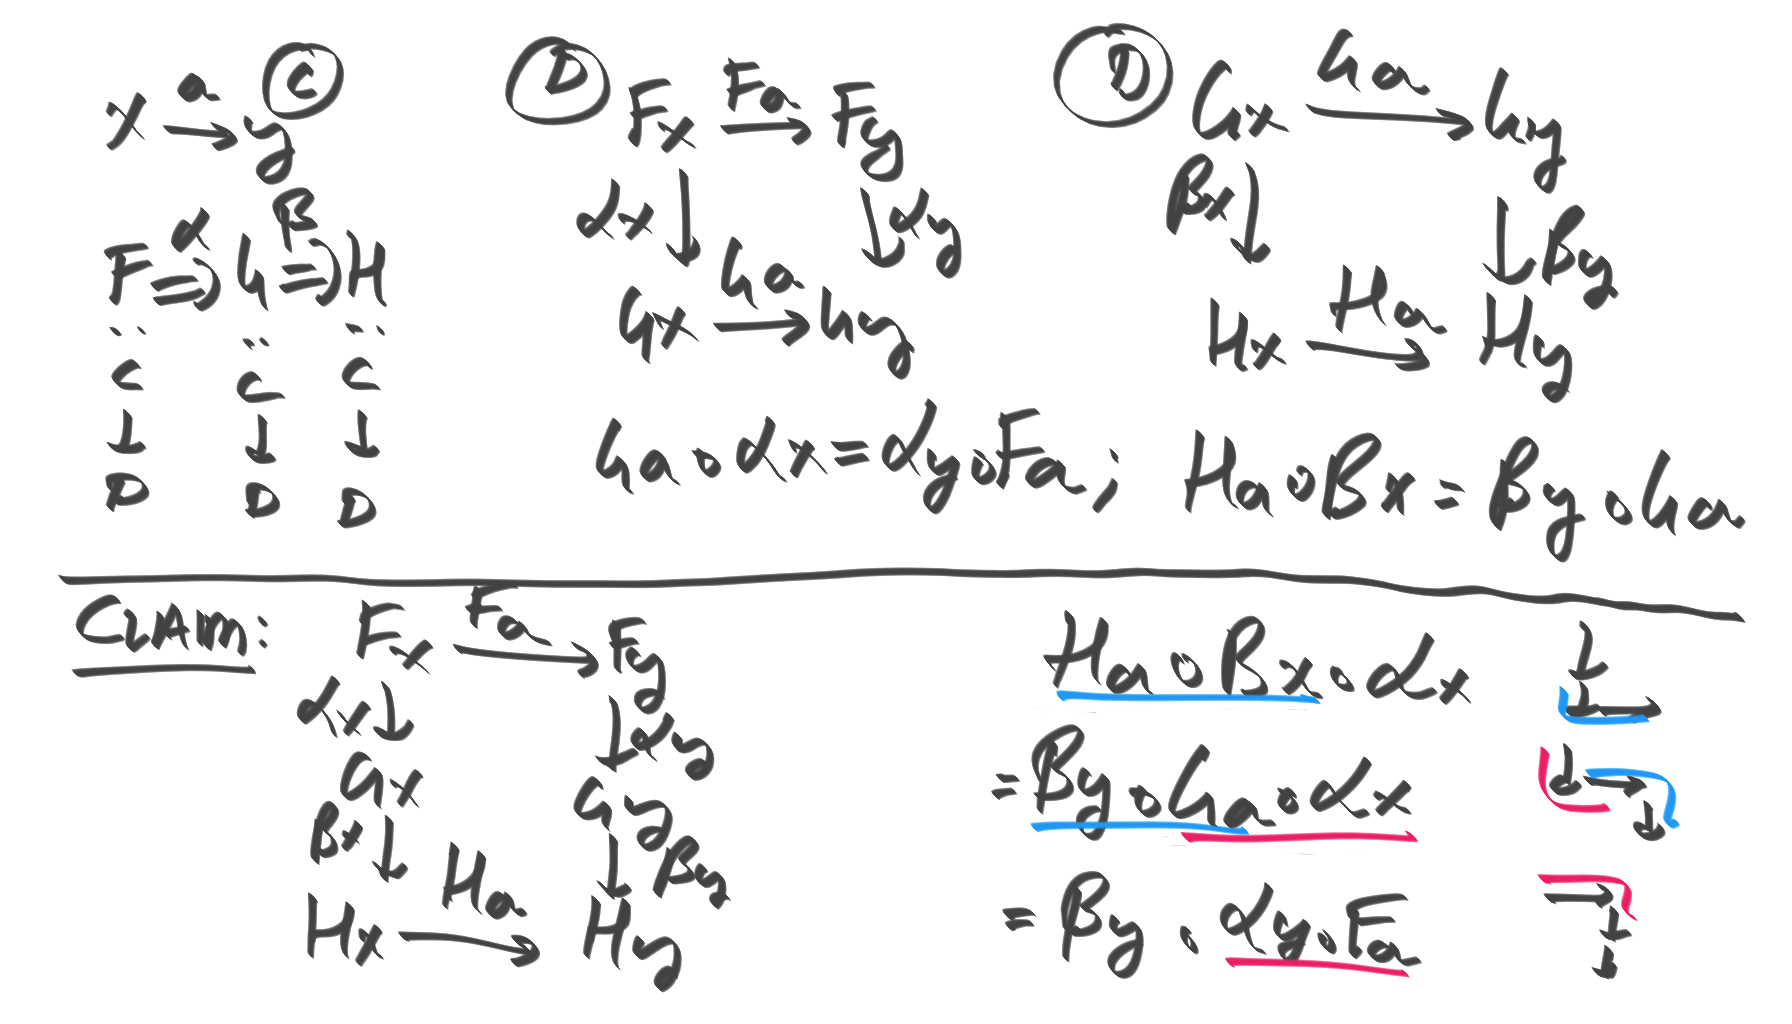
\includegraphics[width=\textwidth]{./ch1/vertical-composition-natural-transformation.png}

The idea is to rewrite the arrows in the down-then-right side of the square (in blue) given by
$H_\alpha \circ \beta_x \circ \alpha_x$ into the right-then-down side of the square (in pink)
given by $\beta_y \circ \alpha_y \circ F_a$. To perorm the rewrite, we apply the naturality
of $\alpha$ and $\beta$.

\subsection{Horizontal Composition}

% https://q.uiver.app/?q=WzAsNixbMCwwLCJDIl0sWzIsMCwiRCJdLFs0LDAsIkUiXSxbNiwwLCJDIl0sWzgsMCwiRSJdLFs1LDAsIlxcbWFwc3RvIl0sWzAsMSwiRyIsMCx7ImN1cnZlIjo1fV0sWzAsMSwiRiIsMix7ImN1cnZlIjotNX1dLFsxLDIsIlEiLDAseyJjdXJ2ZSI6NX1dLFsxLDIsIlAiLDIseyJjdXJ2ZSI6LTV9XSxbMyw0LCJQIFxcY2lyYyBGIiwyLHsiY3VydmUiOi01fV0sWzMsNCwiUSBcXGNpcmMgRyIsMCx7ImN1cnZlIjo1fV0sWzksOCwiXFxiZXRhIiwyLHsic2hvcnRlbiI6eyJzb3VyY2UiOjIwLCJ0YXJnZXQiOjIwfX1dLFs3LDYsIlxcYWxwaGEiLDIseyJzaG9ydGVuIjp7InNvdXJjZSI6MjAsInRhcmdldCI6MjB9fV0sWzEwLDExLCJcXGJldGEqXFxhbHBoYSIsMix7InNob3J0ZW4iOnsic291cmNlIjoyMCwidGFyZ2V0IjoyMH19XV0=
\[\begin{tikzcd}
	C && D && E & \mapsto & C && E
	\arrow[""{name=0, anchor=center, inner sep=0}, "G", curve={height=30pt}, from=1-1, to=1-3]
	\arrow[""{name=1, anchor=center, inner sep=0}, "F"', curve={height=-30pt}, from=1-1, to=1-3]
	\arrow[""{name=2, anchor=center, inner sep=0}, "Q", curve={height=30pt}, from=1-3, to=1-5]
	\arrow[""{name=3, anchor=center, inner sep=0}, "P"', curve={height=-30pt}, from=1-3, to=1-5]
	\arrow[""{name=4, anchor=center, inner sep=0}, "{P \circ F}"', curve={height=-30pt}, from=1-7, to=1-9]
	\arrow[""{name=5, anchor=center, inner sep=0}, "{Q \circ G}", curve={height=30pt}, from=1-7, to=1-9]
	\arrow["\beta"', shorten <=8pt, shorten >=8pt, Rightarrow, from=3, to=2]
	\arrow["\alpha"', shorten <=8pt, shorten >=8pt, Rightarrow, from=1, to=0]
	\arrow["{\beta*\alpha}"', shorten <=8pt, shorten >=8pt, Rightarrow, from=4, to=5]
      \end{tikzcd}\]

We are trying to define the horizontal composition, given by $\beta * \alpha: PF \nt GQ$.
First note that we have $2 \times 2 \times 2$ parameters: $\{P, Q\}$, $\{F, G\}$, and $\{x, y\}$. This is best arranged in a cube:

% https://q.uiver.app/?q=WzAsMTAsWzAsMiwiXFxidWxsZXQiXSxbMSwyXSxbMiwwLCJcXGJ1bGxldCJdLFsyLDIsIlxcYnVsbGV0Il0sWzAsNCwiXFxidWxsZXQiXSxbMSwzLCJcXGJ1bGxldCJdLFsxLDEsIlxcYnVsbGV0Il0sWzMsMSwiXFxidWxsZXQiXSxbMiw0LCJcXGJ1bGxldCJdLFszLDMsIlxcYnVsbGV0Il0sWzAsM10sWzAsNF0sWzQsNV0sWzAsNl0sWzYsNV0sWzYsN10sWzMsN10sWzQsOF0sWzgsOV0sWzUsOV0sWzcsOV0sWzMsOF1d
\[\begin{tikzcd}
	&& \bullet \\
	& \bullet && \bullet \\
	\bullet & {} & \bullet \\
	& \bullet && \bullet \\
	\bullet && \bullet
	\arrow[from=3-1, to=3-3]
	\arrow[from=3-1, to=5-1]
	\arrow[from=5-1, to=4-2]
	\arrow[from=3-1, to=2-2]
	\arrow[from=2-2, to=4-2]
	\arrow[from=2-2, to=2-4]
	\arrow[from=3-3, to=2-4]
	\arrow[from=5-1, to=5-3]
	\arrow[from=5-3, to=4-4]
	\arrow[from=4-2, to=4-4]
	\arrow[from=2-4, to=4-4]
	\arrow[from=3-3, to=5-3]
      \end{tikzcd}\]

First fill up $\{P, Q\}$:

    % https://q.uiver.app/?q=WzAsMTAsWzAsMiwiUCJdLFsxLDJdLFsyLDAsIlxcYnVsbGV0Il0sWzIsMiwiUCJdLFswLDQsIlAiXSxbMSwzLCJRIl0sWzEsMSwiUSJdLFszLDEsIlEiXSxbMiw0LCJQIl0sWzMsMywiUSJdLFswLDNdLFswLDRdLFs0LDVdLFswLDZdLFs2LDVdLFs2LDddLFszLDddLFs0LDhdLFs4LDldLFs1LDldLFs3LDldLFszLDhdXQ==
\[\begin{tikzcd}
	&& \bullet \\
	& Q && Q \\
	P & {} & P \\
	& Q && Q \\
	P && P
	\arrow[from=3-1, to=3-3]
	\arrow[from=3-1, to=5-1]
	\arrow[from=5-1, to=4-2]
	\arrow[from=3-1, to=2-2]
	\arrow[from=2-2, to=4-2]
	\arrow[from=2-2, to=2-4]
	\arrow[from=3-3, to=2-4]
	\arrow[from=5-1, to=5-3]
	\arrow[from=5-3, to=4-4]
	\arrow[from=4-2, to=4-4]
	\arrow[from=2-4, to=4-4]
	\arrow[from=3-3, to=5-3]
\end{tikzcd}\]


Next fill up $\{F, G\}$:
% https://q.uiver.app/?q=WzAsMTAsWzAsMiwiUEYiXSxbMSwyXSxbMiwwLCJcXGJ1bGxldCJdLFsyLDIsIlBHIl0sWzAsNCwiUEYiXSxbMSwzLCJRRiJdLFsxLDEsIlFGIl0sWzMsMSwiUUciXSxbMiw0LCJQRyJdLFszLDMsIlFHIl0sWzAsM10sWzAsNF0sWzQsNV0sWzAsNl0sWzYsNV0sWzYsN10sWzMsN10sWzQsOF0sWzgsOV0sWzUsOV0sWzcsOV0sWzMsOF1d
\[\begin{tikzcd}
	&& \bullet \\
	& QF && QG \\
	PF & {} & PG \\
	& QF && QG \\
	PF && PG
	\arrow[from=3-1, to=3-3]
	\arrow[from=3-1, to=5-1]
	\arrow[from=5-1, to=4-2]
	\arrow[from=3-1, to=2-2]
	\arrow[from=2-2, to=4-2]
	\arrow[from=2-2, to=2-4]
	\arrow[from=3-3, to=2-4]
	\arrow[from=5-1, to=5-3]
	\arrow[from=5-3, to=4-4]
	\arrow[from=4-2, to=4-4]
	\arrow[from=2-4, to=4-4]
	\arrow[from=3-3, to=5-3]
      \end{tikzcd}\]

Finally, fill up $\{x, y\}$:
% \includegraphics[width=\textwidth]{./ch1/horizontal-composition.png}

% https://q.uiver.app/?q=WzAsMTAsWzAsMiwiUEZ4Il0sWzEsMl0sWzIsMCwiXFxidWxsZXQiXSxbMiwyLCJQR3giXSxbMCw0LCJQRnkiXSxbMSwzLCJRRnkiXSxbMSwxLCJRRngiXSxbMywxLCJRR3giXSxbMiw0LCJQR3kiXSxbMywzLCJRR3kiXSxbMCwzXSxbMCw0XSxbNCw1XSxbMCw2XSxbNiw1XSxbNiw3XSxbMyw3XSxbNCw4XSxbOCw5XSxbNSw5XSxbNyw5XSxbMyw4XV0=
\[\begin{tikzcd}
	&& \bullet \\
	& QFx && QGx \\
	PFx & {} & PGx \\
	& QFy && QGy \\
	PFy && PGy
	\arrow[from=3-1, to=3-3]
	\arrow[from=3-1, to=5-1]
	\arrow[from=5-1, to=4-2]
	\arrow[from=3-1, to=2-2]
	\arrow[from=2-2, to=4-2]
	\arrow[from=2-2, to=2-4]
	\arrow[from=3-3, to=2-4]
	\arrow[from=5-1, to=5-3]
	\arrow[from=5-3, to=4-4]
	\arrow[from=4-2, to=4-4]
	\arrow[from=2-4, to=4-4]
	\arrow[from=3-3, to=5-3]
      \end{tikzcd}\]

    First, let's define $(\beta * \alpha)(\bullet) : PF \bullet \rightarrow QG \bullet$ as the
    composition of the arrows:

$$
PF \bullet \xrightarrow{P \alpha \bullet} PG \bullet \xrightarrow{\beta (G \bullet)} QG \bullet
$$

That is, $(\beta * \alpha)(\bullet) : PF \bullet \rightarrow QG \bullet \equiv \equiv \beta(G\bullet) \circ P(\alpha \bullet)$. 

    
\subsection{Exercises}

\start{Question 1.7.i} If $C$ is small, $D$ locally small, then $D^C$ is locally small
\start{Answer}
Recall that $D^C$ has as objects as fuctors $F, G: C \rightarrow D$, and as arrows has natural transformations $\eta: F \nt G \in Hom(F, G)$.
Recall that a natural transformation assigns to each object $c \in C$ an arrow $\eta_c: Fc \rightarrow Gc \in Hom_D(Fc, Gc)$. So if we consider
all natural transformations, the data is given by a choice function, which for every  $c \in C$ assigns an element in $Hom_D(Fc, Gc)$.
Since $C$ is small, the collection $c \in C$ is a set. Since $D$ is locally small, the set $Hom_D(Fc, Gc)$ is a set. Thus, the data
of all natural transformations is expressed by:

$$ Hom(F, G) \equiv  \prod_{c \in C} Hom_D(Fc, Gc) $$

This is not exactly a natural transformation, since this does not enfore the coherence conditions. So this is a super-collection
of the scollection of all natural transformations. We see that is a well defined set-theoretic expression, since $C$ is small, it is legal to range over it,
and since $D$ is locally small, it is legal to invoke $Hom_D(Fc, Gc)$ as a set. Thus, the full $Hom(F, G)$ is a set.


\start{Question 1.7.ii} Given $C \xrightarrow{F} D \xrightarrow{H \nt K} E \xrightarrow{L} F$, where $\eta: H \nt E$, define
a natural transformation $L \beta F : LHF \rightarrow LKF$ given by $(L \beta F)(\bullet) \equiv L(\beta(F(\bullet))$.
Prove that $L \beta F$ is indeed
natural (ie, that the appropriate diagram commutes)

\start{Answer} We start by considering an arrow $x \xrightarrow{a} y \in C$. By applying $F$, we get $Fx \xrightarrow{Fa} Fy \in D$.
Next, to get access to $\beta: H \nt K$, we start by using $H$ to get $HFx \xrightarrow{HFa} HFy \in E$. We use the naturality
of $\beta$ to transform to draw the commutative square with $HF$ and $KF$, linked by $\eta$. This diagram lives in $E$
and commutes by the naturality of $\beta$. Finally, we apply $L$ to send a commutative diagram to another commutative diagram
in $F$, with the natural transformation between $LHF$ and $LKF$. Hence, naturality is proven.

% https://q.uiver.app/?q=WzAsMTksWzAsMCwieCJdLFsxLDAsInkiXSxbMCwxLCJGeCJdLFsxLDEsIkZ5Il0sWzAsMiwiSEZ4Il0sWzEsMiwiSEZ5Il0sWzAsMywiSChGeCkiXSxbMSwzLCJIKEZ5KSJdLFswLDQsIksoRngpIl0sWzEsNCwiSyhGeSkiXSxbMCw2LCJMKEgoRngpKSJdLFsxLDYsIkwoSyhGeCkpIl0sWzAsNywiTChLKEZ4KSkiXSxbMSw3LCJMKEsoRnkpKSJdLFszLDAsIlxcdGV4dHthcmJpdHJhcnkgYXJyb3cgaW4gfSBDIl0sWzMsMSwiXFx0ZXh0e2FwcGx5IH0gRiBcXHRleHR7IHRvIGxhbmQgaW4gfSBEIl0sWzMsMiwiXFx0ZXh0e2FwcGx5IH0gSCBcXHRleHR7IHRvIGxhbmQgaW4gfSBFIl0sWzMsMywiXFx0ZXh0e05hdHVyYWxpdHkgb2YgfSBcXGJldGEiXSxbMyw2LCJcXHRleHR7YXBwbHkgfSBMIFxcdGV4dHsgdG8gbGFuZCBpbiB9IEYiXSxbMCwxLCJhIl0sWzIsMywiRmEiXSxbNCw1LCJIRmEiXSxbNiw3LCJIKEZhKSJdLFs2LDgsIlxcYmV0YShGeCkiLDJdLFs3LDksIlxcYmV0YShGeSkiXSxbOCw5LCJLKEZhKSIsMl0sWzEwLDExLCJMKEgoRmEpKSJdLFsxMCwxMiwiTChcXGJldGEoRngpKSIsMl0sWzEyLDEzXSxbMTEsMTMsIkwoXFxiZXRhKEZ5KSkiXV0=
\[\begin{tikzcd}
	x & y && {\text{arbitrary arrow in } C} \\
	Fx & Fy && {\text{apply } F \text{ to land in } D} \\
	HFx & HFy && {\text{apply } H \text{ to land in } E} \\
	{H(Fx)} & {H(Fy)} && {\text{Naturality of } \beta} \\
	{K(Fx)} & {K(Fy)} \\
	\\
	{L(H(Fx))} & {L(K(Fx))} && {\text{apply } L \text{ to land in } F} \\
	{L(K(Fx))} & {L(K(Fy))}
	\arrow["a", from=1-1, to=1-2]
	\arrow["Fa", from=2-1, to=2-2]
	\arrow["HFa", from=3-1, to=3-2]
	\arrow["{H(Fa)}", from=4-1, to=4-2]
	\arrow["{\beta(Fx)}"', from=4-1, to=5-1]
	\arrow["{\beta(Fy)}", from=4-2, to=5-2]
	\arrow["{K(Fa)}"', from=5-1, to=5-2]
	\arrow["{L(H(Fa))}", from=7-1, to=7-2]
	\arrow["{L(\beta(Fx))}"', from=7-1, to=8-1]
	\arrow[from=8-1, to=8-2]
	\arrow["{L(\beta(Fy))}", from=7-2, to=8-2]
\end{tikzcd}\]

\start{Question 1.7.iii} Redefine horizontal composition using vertical composition and whiskering.
Given $C \xrightarrow{F \nt G} D \xrightarrow {P \nt Q} E$, where the natural transformations are $\alpha: F \nt G$
and $\beta: P \nt Q$, we wish to define $\beta * \alpha : PF \nt QG$. 

\start{Answer}  TODO. I have no idea what the question wants us to do.


\start{Question 1.7.iv} Prove 1.7.7 (Middle four interchange), that states that $(\beta \circ \alpha) * (\delta \circ \gamma)$ 
equals $(\gamma * \alpha) \circ (\delta * \beta)$.
\start{Answer} Recall that $(\omega : C \xrightarrow{F \nt G} D * \phi : D \xrightarrow{P \nt Q} E) : D \xrightarrow{PF \nt QG} E$ is defined as 
$(\omega * \phi) : PF \bullet \rightarrow QG \bullet$  given by:

% https://q.uiver.app/?q=WzAsNyxbMCwwLCJQRlxcYnVsbGV0Il0sWzIsMCwiUEdcXGJ1bGxldCJdLFsyLDIsIlFHXFxidWxsZXQiXSxbMCwyLCJRRlxcYnVsbGV0Il0sWzEsNCwiXFxwaGk6IEZcXGJ1bGxldCBcXHJpZ2h0YXJyb3cgR1xcYnVsbGV0Il0sWzEsMywiXFxvbWVnYTogUFxcYnVsbGV0IFxccmlnaHRhcnJvdyBRIFxcYnVsbGV0Il0sWzEsMSwiXFxjaXJjbGVhcnJvd3JpZ2h0IDogIFxcdGV4dHtuYXR1cmFsaXR5IG9mIH0gXFxvbWVnYSJdLFswLDEsIlAoXFxwaGkgIFxcYnVsbGV0KSJdLFsxLDIsIlxcb21lZ2EoR1xcYnVsbGV0KSJdLFswLDMsIlxcb21lZ2EoRlxcYnVsbGV0KSIsMl0sWzMsMiwiUShcXHBoaSBcXGJ1bGxldCkiLDJdLFswLDIsIihcXG9tZWdhICogXFxwaGkpIChcXGJ1bGxldCkiLDEseyJvZmZzZXQiOi0xLCJjdXJ2ZSI6NCwic3R5bGUiOnsiYm9keSI6eyJuYW1lIjoic3F1aWdnbHkifX19XV0=
\[\begin{tikzcd}
	PF\bullet && PG\bullet \\
	& {\circlearrowright :  \text{naturality of } \omega} \\
	QF\bullet && QG\bullet \\
	& {\omega: P\bullet \rightarrow Q \bullet} \\
	& {\phi: F\bullet \rightarrow G\bullet}
	\arrow["{P(\phi  \bullet)}", from=1-1, to=1-3]
	\arrow["{\omega(G\bullet)}", from=1-3, to=3-3]
	\arrow["{\omega(F\bullet)}"', from=1-1, to=3-1]
	\arrow["{Q(\phi \bullet)}"', from=3-1, to=3-3]
	\arrow["{(\omega * \phi) (\bullet)}"{description}, shift left=1, curve={height=24pt}, squiggly, from=1-1, to=3-3]
\end{tikzcd}\]

Consider the large commutative diagram:

% https://q.uiver.app/?q=WzAsMTMsWzAsMCwiUEZcXGJ1bGxldCJdLFsyLDAsIlBHIFxcYnVsbGV0Il0sWzQsMCwiUEggXFxidWxsZXQiXSxbMCwyLCJRRiBcXGJ1bGxldCJdLFsyLDIsIlFHIFxcYnVsbGV0Il0sWzQsMiwiUUggXFxidWxsZXQiXSxbMCw0LCJSRiBcXGJ1bGxldCJdLFsyLDQsIlJHIFxcYnVsbGV0Il0sWzQsNCwiUkggXFxidWxsZXQiXSxbMSwxLCJcXHRleHR7bmF0dXJhbGl0eSBvZiB9IFxcZ2FtbWEiXSxbMywxLCJcXHRleHR7bmF0dXJhbGl0eSBvZiB9IFxcZ2FtbWEiXSxbMSwzLCJcXHRleHR7bmF0dXJhbGl0eSBvZiB9IFxcZGVsdGEiXSxbMywzLCJcXHRleHR7bmF0dXJhbGl0eSBvZiB9IFxcZGVsdGEiXSxbMCwxLCJQKFxcYWxwaGEgXFxidWxsZXQpIl0sWzEsMiwiUChcXGJldGEgXFxidWxsZXQpIl0sWzMsNCwiUShcXGFscGhhIFxcYnVsbGV0KSJdLFs2LDcsIlIoXFxhbHBoYSBcXGJ1bGxldCkiXSxbNCw1LCJRKFxcYmV0YSBcXGJ1bGxldCkiXSxbNyw4LCJSKFxcYmV0YSBcXGJ1bGxldCkiXSxbMCwzLCJcXGdhbW1hKEZcXGJ1bGxldCkiLDFdLFsxLDQsIlxcZ2FtbWEoR1xcYnVsbGV0KSIsMV0sWzIsNSwiXFxnYW1tYShIXFxidWxsZXQpIiwxXSxbMyw2LCJcXGRlbHRhKEYgXFxidWxsZXQpIiwxXSxbNCw3LCJcXGRlbHRhKEcgXFxidWxsZXQpIiwxXSxbNSw4LCJcXGRlbHRhKEggXFxidWxsZXQpIiwxXV0=
\[\begin{tikzcd}
	PF\bullet && {PG \bullet} && {PH \bullet} \\
	& {\text{naturality of } \gamma} && {\text{naturality of } \gamma} \\
	{QF \bullet} && {QG \bullet} && {QH \bullet} \\
	& {\text{naturality of } \delta} && {\text{naturality of } \delta} \\
	{RF \bullet} && {RG \bullet} && {RH \bullet}
	\arrow["{P(\alpha \bullet)}", from=1-1, to=1-3]
	\arrow["{P(\beta \bullet)}", from=1-3, to=1-5]
	\arrow["{Q(\alpha \bullet)}", from=3-1, to=3-3]
	\arrow["{R(\alpha \bullet)}", from=5-1, to=5-3]
	\arrow["{Q(\beta \bullet)}", from=3-3, to=3-5]
	\arrow["{R(\beta \bullet)}", from=5-3, to=5-5]
	\arrow["{\gamma(F\bullet)}"{description}, from=1-1, to=3-1]
	\arrow["{\gamma(G\bullet)}"{description}, from=1-3, to=3-3]
	\arrow["{\gamma(H\bullet)}"{description}, from=1-5, to=3-5]
	\arrow["{\delta(F \bullet)}"{description}, from=3-1, to=5-1]
	\arrow["{\delta(G \bullet)}"{description}, from=3-3, to=5-3]
	\arrow["{\delta(H \bullet)}"{description}, from=3-5, to=5-5]
\end{tikzcd}\]

By composing the outer morphisms, we get:

% https://q.uiver.app/?q=WzAsNCxbMCwwLCJQRlxcYnVsbGV0Il0sWzAsMywiUkZcXGJ1bGxldCJdLFs0LDMsIlJIXFxidWxsZXQiXSxbNCwwLCJQSFxcYnVsbGV0Il0sWzAsMSwiKFxcZGVsdGEgXFxjaXJjIFxcZ2FtbWEpKEYgXFxidWxsZXQpIiwyXSxbMSwyLCJSKChcXGJldGEgXFxjaXJjIFxcYWxwaGEgKVxcYnVsbGV0KSIsMl0sWzAsMywiUCgoXFxiZXRhIFxcY2lyYyBcXGFscGhhIClcXGJ1bGxldCkiXSxbMywyLCIoXFxkZWx0YSBcXGNpcmMgXFxnYW1tYSkoSCBcXGJ1bGxldCkiXSxbMCwyLCIoXFxnYW1tYSBcXGNpcmMgXFxkZWx0YSkgKiAoXFxiZXRhIFxcY2lyYyBcXGFscGhhKSIsMSx7InN0eWxlIjp7ImJvZHkiOnsibmFtZSI6InNxdWlnZ2x5In19fV1d
\[\begin{tikzcd}
	PF\bullet &&&& PH\bullet \\
	\\
	\\
	RF\bullet &&&& RH\bullet
	\arrow["{(\delta \circ \gamma)(F \bullet)}"', from=1-1, to=4-1]
	\arrow["{R((\beta \circ \alpha )\bullet)}"', from=4-1, to=4-5]
	\arrow["{P((\beta \circ \alpha )\bullet)}", from=1-1, to=1-5]
	\arrow["{(\delta \circ \gamma)(H \bullet)}", from=1-5, to=4-5]
	\arrow["{(\gamma \circ \delta) * (\beta \circ \alpha)}"{description}, squiggly, from=1-1, to=4-5]
\end{tikzcd}\]

By composing the inner morphisms, we get $(\gamma * \alpha) \circ (\delta * \beta)$

% https://q.uiver.app/?q=WzAsMTMsWzAsMCwiUEZcXGJ1bGxldCJdLFszLDAsIlBHIFxcYnVsbGV0Il0sWzYsMCwiUEggXFxidWxsZXQiXSxbMCwzLCJRRiBcXGJ1bGxldCJdLFszLDMsIlFHIFxcYnVsbGV0Il0sWzYsMywiUUggXFxidWxsZXQiXSxbMCw2LCJSRiBcXGJ1bGxldCJdLFszLDYsIlJHIFxcYnVsbGV0Il0sWzYsNiwiUkggXFxidWxsZXQiXSxbMSwyLCJcXGNpcmNsZWFycm93cmlnaHQgXFx0ZXh0e25hdC4gfSBcXGdhbW1hIl0sWzQsMiwiXFxjaXJjbGVhcnJvd3JpZ2h0IFxcdGV4dHtuYXQuIH0gXFxnYW1tYSJdLFsxLDUsIlxcY2lyY2xlYXJyb3dyaWdodCBcXHRleHR7bmF0LiAgfSBcXGRlbHRhIl0sWzQsNSwiXFxjaXJjbGVhcnJvd3JpZ2h0IFxcdGV4dHtuYXQuIH0gXFxkZWx0YSJdLFswLDEsIlAoXFxhbHBoYSBcXGJ1bGxldCkiXSxbMSwyLCJQKFxcYmV0YSBcXGJ1bGxldCkiLDAseyJzdHlsZSI6eyJib2R5Ijp7Im5hbWUiOiJkYXNoZWQifX19XSxbMyw0LCJRKFxcYWxwaGEgXFxidWxsZXQpIiwyXSxbNiw3LCJSKFxcYWxwaGEgXFxidWxsZXQpIiwwLHsic3R5bGUiOnsiYm9keSI6eyJuYW1lIjoiZGFzaGVkIn19fV0sWzQsNSwiUShcXGJldGEgXFxidWxsZXQpIl0sWzcsOCwiUihcXGJldGEgXFxidWxsZXQpIl0sWzAsMywiXFxnYW1tYShGXFxidWxsZXQpIiwxXSxbMSw0LCJcXGdhbW1hKEdcXGJ1bGxldCkiLDFdLFsyLDUsIlxcZ2FtbWEoSFxcYnVsbGV0KSIsMSx7InN0eWxlIjp7ImJvZHkiOnsibmFtZSI6ImRhc2hlZCJ9fX1dLFszLDYsIlxcZGVsdGEoRiBcXGJ1bGxldCkiLDEseyJzdHlsZSI6eyJib2R5Ijp7Im5hbWUiOiJkYXNoZWQifX19XSxbNCw3LCJcXGRlbHRhKEcgXFxidWxsZXQpIiwxXSxbNSw4LCJcXGRlbHRhKEggXFxidWxsZXQpIiwxXSxbMCw0LCIoXFxnYW1tYSAqIFxcYWxwaGEpKFxcYnVsbGV0KSIsMCx7ImxhYmVsX3Bvc2l0aW9uIjo2MCwic3R5bGUiOnsiYm9keSI6eyJuYW1lIjoic3F1aWdnbHkifX19XSxbNCw4LCIoXFxkZWx0YSAqIFxcYmV0YSkoXFxidWxsZXQpIiwwLHsic3R5bGUiOnsiYm9keSI6eyJuYW1lIjoic3F1aWdnbHkifX19XV0=
\[\begin{tikzcd}
	PF\bullet &&& {PG \bullet} &&& {PH \bullet} \\
	\\
	& {\circlearrowright \text{nat. } \gamma} &&& {\circlearrowright \text{nat. } \gamma} \\
	{QF \bullet} &&& {QG \bullet} &&& {QH \bullet} \\
	\\
	& {\circlearrowright \text{nat.  } \delta} &&& {\circlearrowright \text{nat. } \delta} \\
	{RF \bullet} &&& {RG \bullet} &&& {RH \bullet}
	\arrow["{P(\alpha \bullet)}", from=1-1, to=1-4]
	\arrow["{P(\beta \bullet)}", dashed, from=1-4, to=1-7]
	\arrow["{Q(\alpha \bullet)}"', from=4-1, to=4-4]
	\arrow["{R(\alpha \bullet)}", dashed, from=7-1, to=7-4]
	\arrow["{Q(\beta \bullet)}", from=4-4, to=4-7]
	\arrow["{R(\beta \bullet)}", from=7-4, to=7-7]
	\arrow["{\gamma(F\bullet)}"{description}, from=1-1, to=4-1]
	\arrow["{\gamma(G\bullet)}"{description}, from=1-4, to=4-4]
	\arrow["{\gamma(H\bullet)}"{description}, dashed, from=1-7, to=4-7]
	\arrow["{\delta(F \bullet)}"{description}, dashed, from=4-1, to=7-1]
	\arrow["{\delta(G \bullet)}"{description}, from=4-4, to=7-4]
	\arrow["{\delta(H \bullet)}"{description}, from=4-7, to=7-7]
	\arrow["{(\gamma * \alpha)(\bullet)}"{pos=0.6}, squiggly, from=1-1, to=4-4]
	\arrow["{(\delta * \beta)(\bullet)}", squiggly, from=4-4, to=7-7]
\end{tikzcd}\]


By the commutativity of the large square, these two are equal, and hence the four composition
theorem holds.

\question{1.7.v} Show that the
collection of natural transformations of the form $\{ 1_C \nt 1_C \}$  defines a commutative monoid (under vertical composition).

Consider such a natural transformation $\alpha: 1_C \nt 1_C$. From naturality, for all arrows $x \xrightarrow{a} y$, 
$\alpha$ must satisfy $a \circ \alpha(x) = \alpha(y) \circ a$:

% https://q.uiver.app/?q=WzAsMTIsWzAsMSwiMV9DeCJdLFsyLDEsIjFfQ3kiXSxbMCwzLCIxX0N4Il0sWzIsMywiMV9DeSJdLFswLDAsIngiXSxbMiwwLCJ5Il0sWzEsMiwiIFxcY2lyY2xlYXJyb3dyaWdodCBcXHRleHR7bmF0IH0gXFxhbHBoYSAgIl0sWzAsNCwieCJdLFsyLDQsInkiXSxbMCw2LCJ4Il0sWzIsNiwieSJdLFsxLDUsImEgXFxjaXJjIFxcYWxwaGEoeCkgPSBcXGFscGhhKHkpIFxcY2lyYyBhIl0sWzAsMSwiMV9DIGEiXSxbMCwyLCJcXGFscGhhIHgiLDJdLFsyLDMsIjFfQyBhIiwyXSxbMSwzLCJcXGFscGhhIHkiXSxbNCw1LCJhIiwyXSxbNyw4LCJhIiwyXSxbNyw5LCJcXGFscGhhIHgiLDJdLFs5LDEwLCJhIl0sWzgsMTAsIlxcYWxwaGEgeSIsMl1d
\[\begin{tikzcd}
	x && y \\
	{1_Cx} && {1_Cy} \\
	& { \circlearrowright \text{nat } \alpha  } \\
	{1_Cx} && {1_Cy} \\
	x && y \\
	& {a \circ \alpha(x) = \alpha(y) \circ a} \\
	x && y
	\arrow["{1_C a}", from=2-1, to=2-3]
	\arrow["{\alpha x}"', from=2-1, to=4-1]
	\arrow["{1_C a}"', from=4-1, to=4-3]
	\arrow["{\alpha y}", from=2-3, to=4-3]
	\arrow["a"', from=1-1, to=1-3]
	\arrow["a"', from=5-1, to=5-3]
	\arrow["{\alpha x}"', from=5-1, to=7-1]
	\arrow["a", from=7-1, to=7-3]
	\arrow["{\alpha y}"', from=5-3, to=7-3]
\end{tikzcd}\]

\begin{itemize}
\item given two $\alpha, \beta: 1_C \nt 1_C$, we must have that $\alpha(x) \circ \beta(x) = \beta(x) \circ \alpha(x)$ [since $\alpha(x) \circ a = a \circ \alpha(y)]$.
\item Since this holds at all points, we get $\alpha \circ \beta = \beta \circ \alpha$, or that these are commutative.
    \item The identity natural transformation
$e$ given by $e(1_C x) = e(x) \equiv x = 1_C x$  is the identity for the monoid of endo-natural transformations of the functor $1_C$. Verification is formal,
and left to be jotted down to future Siddharth.
\end{itemize}

    
\question{1.7.vi}  TODO

\question{1.7.vii} Show that a bifunction $F: C \times D \rightarrow E$ is equivalent to the data:
\begin{itemize}
    \item A functor $F(c, -): D \rightarrow E$ for each $c \in C$
    \item A natural transformation $F(f, -): F(x, -) \nt F(y, -)$ for each
    $x \xrightarrow{f} y \in C$, defined functorially in $C$ \item To be ``defined
        functorially'' is to say that we have a functor $G: C \rightarrow D^E$,
        which is in bijection with $F: C \times D \rightarrow E$.
\end{itemize}
\start{Answer ($\implies$): Bifunctor implies partial application}
\begin{itemize}
\item Given a bifunctor $F$, define for each $c \in C$ a funtor $\partial F(c, -): D \rightarrow E$
\item On objects, we define $\partial F(c, -)(d) \equiv F(c, d)$
\item On arrows, we define $\partial F(c, -) (x \xrightarrow{g} y) \equiv  F(1_c, g)$.
\item See that the definition on objects and arrows is consistent:

% https://q.uiver.app/?q=WzAsNixbMCwwLCJ4IFxcaW4gRCJdLFsyLDAsInkgXFxpbiBEIl0sWzAsMSwiXFxwYXJ0aWFsIEYoYywtKSh4KSBcXGluIEUiXSxbMiwxLCJcXHBhcnRpYWwgRihjLC0pKHkpIFxcaW4gRSJdLFswLDIsIkYoYywgeCkiXSxbMiwyLCJGKGMsIHkpIl0sWzAsMSwiZyJdLFsyLDMsIlxccGFydGlhbCBGKGMsIC0pKGcpIl0sWzQsNSwiRigxX2MsIGcpIl1d
\[\begin{tikzcd}
	{x \in D} && {y \in D} \\
	{\partial F(c,-)(x) \in E} && {\partial F(c,-)(y) \in E} \\
	{F(c, x)} && {F(c, y)}
	\arrow["g", from=1-1, to=1-3]
	\arrow["{\partial F(c, -)(g)}", from=2-1, to=2-3]
	\arrow["{F(\id_c, g)}", from=3-1, to=3-3]
\end{tikzcd}\]

\item See that $\partial F(c, -)$ preserves identity:
\begin{align*}
    & \partial F(c, -)(\id_d) \\
    & = F(\id_c, \id_d) \quad \text{(Defn of $\partial F(c, -)$}
    & = id_{F(c, d)} \quad \text{(Functoriality of $F$)}
\end{align*}

\item See that $\partial F(c, -)$ distributes over $\circ$:
\begin{align*}
    & \partial F(c, -)(x \xrightarrow{f} y\xrightarrow{g} z) \\
    & = F(\id_c, g \circ_D f) \quad \text{(Defn of $\partial F(c, -)$) }\\
    &= F(\id_c \circ_C id_c, g \circ_D f) \quad \text{($h \circ id_c = id_c$)  } \\
    &= F((\id_c, g) \circ_{C \times D} (id_c, f)) \quad \text{(Defn. of composition in $C \times D$)} \\
    &= F((\id_c, g)) \circ_{E} F((id_c, f)) \quad \text{(Functoriality of $F$)}\\
    &= \partial F(c, -)(g) \circ_{E} \partial F(c, -)(f) \quad \text{(Defn of $\partial F(c, -)$)}\\
\end{align*}

\item This completes our verification that $\partial F(c -)$ is a functor. 
\item We move to constructing the natural transformations $\partial F(f, -): \partial F(c, -) \nt \partial F(c', -)$ for each $f: c \rightarrow c'$.
\item The natural transformation assigns components for each $d \in D$. It must produce arrows $\partial F(c, -)(d) \rightarrow \partial F(c', -)(d)$
    which live in $E$. We choose to produce the arrow $F(f, id_d)$. That is, $\partial F(f, -)(d) \equiv F(f, id_d)$. This assembles into a
        square whose commutativity is to be established:

    % https://q.uiver.app/?q=WzAsNyxbMCwwLCJkIl0sWzIsMCwiZCciXSxbMCw0LCJcXHBhcnRpYWwgRihjJywgLSkoZCkiXSxbMCwyLCJcXHBhcnRpYWwgRihjLCAtKShkKSJdLFsyLDIsIlxccGFydGlhbCBGKGMsIC0pKGQnKSJdLFsyLDQsIlxccGFydGlhbCBGKGMnLCAtKShkJykiXSxbMSwzLCJcXGNpcmNsZWFycm93cmlnaHQgPyAiXSxbMCwxLCJhIl0sWzIsNSwiXFxwYXJ0aWFsIEYoYycsIC0pKGEpIl0sWzMsMiwiXFxwYXJ0aWFsIEYoZiwgLSkoZCkiLDJdLFszLDQsIlxccGFydGlhbCBGKGMsIC0pKGEpIl0sWzQsNSwiXFxwYXJ0aWFsIEYoZiwgLSkoZCcpIl1d
\[\begin{tikzcd}
	d && {d'} \\
	\\
	{\partial F(c, -)(d)} && {\partial F(c, -)(d')} \\
	& {\circlearrowright ? } \\
	{\partial F(c', -)(d)} && {\partial F(c', -)(d')}
	\arrow["a", from=1-1, to=1-3]
	\arrow["{\partial F(c', -)(a)}", from=5-1, to=5-3]
	\arrow["{\partial F(f, -)(d)}"', from=3-1, to=5-1]
	\arrow["{\partial F(c, -)(a)}", from=3-1, to=3-3]
	\arrow["{\partial F(f, -)(d')}", from=3-3, to=5-3]
\end{tikzcd}\]
Which upon substituting definitions becomes:

% https://q.uiver.app/?q=WzAsNCxbMCwwLCJGKGMsIGQpIl0sWzIsMCwiRihjLCBkJykiXSxbMCwyLCJGKGMnLCBkKSJdLFsyLDIsIkYoYycsIGQnKSJdLFswLDEsIkYoaWRfYywgYSkiXSxbMCwyLCJGKGYsIGlkX2QpIiwyXSxbMSwzLCJGKGYsIGlkX3tkJ30pIl0sWzIsMywiRihpZF97Yyd9LCBhKSIsMl1d
\[\begin{tikzcd}
	{F(c, d)} && {F(c, d')} \\
	\\
	{F(c', d)} && {F(c', d')}
	\arrow["{F(id_c, a)}", from=1-1, to=1-3]
	\arrow["{F(f, id_d)}"', from=1-1, to=3-1]
	\arrow["{F(f, id_{d'})}", from=1-3, to=3-3]
	\arrow["{F(id_{c'}, a)}"', from=3-1, to=3-3]
\end{tikzcd}\]

Which commutes since $F$ preserves commuting diagrams as it is a functor, and the following diagram commutes
(by direct verification):

% https://q.uiver.app/?q=WzAsNCxbMCwwLCIoYywgZCkiXSxbMiwwLCIoYywgZCcpIl0sWzAsMiwiKGMnLCBkKSJdLFsyLDIsIihjJywgZCcpIl0sWzAsMSwiKGlkX2MsIGEpIl0sWzAsMiwiKGYsIGlkX2QpIiwyXSxbMiwzLCIoaWRfe2MnfSwgYSkiLDJdLFsxLDMsIihmLCBpZF97ZCd9KSJdXQ==
\[\begin{tikzcd}
	{(c, d)} && {(c, d')} \\
	\\
	{(c', d)} && {(c', d')}
	\arrow["{(id_c, a)}", from=1-1, to=1-3]
	\arrow["{(f, id_d)}"', from=1-1, to=3-1]
	\arrow["{(id_{c'}, a)}"', from=3-1, to=3-3]
	\arrow["{(f, id_{d'})}", from=1-3, to=3-3]
\end{tikzcd}\]

\item To prove functoriality of this assignment, we must show that given $d_1 \xrightarrow{a} d_2 \xrightarrow{b} d_3$,
    the equation $\partial F (f, -)(b \circ_D a) = \partial F(f, -)(b) \circ_E \partial F(f, -) a$. This follows by
    computation:
\begin{align*}
& \partial F (f, -)(b \circ_D a) \\
&= 
\end{align*}

\end{itemize}


\chapter{Universal Properties, Representability, The Yoneda Lemma}

\section{Representable Functors}

\subsection{Musing}

Let $F: \cSet \to \cGrp $ and $U: \cGrp \to \cSet$ be adjoints, where $F$ is free and $U$ is forgetful. So we can
translate arrows of the form $Fx \to y$ into arrows $x \to Gy$. Let $1 \equiv \{ * \}$ be the final object in $\cSet$. 
\textbf{Claim}: $F(1): Grp$ is the representing object for the forgetful functor $U: \cGrp \to \cSet$.

For $F(1)$ to be a representing object, there must be a natural isomorphism between the functor $U: \cGrp \to \cSet$ and the functor $Hom(F(1), -): \cGrp \to \cSet$.
So we must establish a natural bijection between $U \bullet$ and $Hom(F(1), \bullet)$ for any group $\bullet$.

See that any morphism $[F(1) \to \bullet]$ is in bijection
with $[1 \to U(\bullet)]$. Morphisms of the form $[1 \to U (\bullet)]$ is isomorphic to $\bullet$, since a map of the form $f: 1 \to U \bullet$
picks out elements of $U\bullet$ $(im(f) = f(*) \in \bullet$).

In a single line, we have:

$$
Hom_{Grp}(F(1), G) \simeq Hom_{Set}(1, UG) \simeq UG
$$


\subsubsection{Proof that functors upto equivalence form a groupoid, with all rewrites witnessed by natural transformations.}


\subsection{Exercises}

\question{2.1.i} Describe natural transformations between (a)
the functors $0: \mathbb 1 \rightarrow mathbb 2$, $1: \mathbb 1 \rightarrow \mathbb 2$, and $!: \mathbb 2 \rightarrow \mathbb 1$ and
(b) the covariant functors $\cCat \to \cSet$ represented by the categories $\mathbb 1$ and $\mathbb 2$, 

TODO: what should we prove? I don't think I understand the question.

\question{2.1.ii} Prove that if $F: \cC \rightarrow \cSet$ is representable then it preserves monomorphisms.
Let $F$ be represented by some $r \in \cC$. So we have a natural isomorphism $\eta: F \rightarrow \Hom_C(r, -)$. Suppose
we have a monomorphism $y \xrightarrow{m} z$. So given any other arrows $f, g: x \rightarrow y$, we have that $m \circ f = m \circ g$ implies $f = g$.

\begin{itemize}
\item Consider the image under $\Hom(r, -)$.
\item We wish to show that if $\Hom(r, -)(m) \circ \Hom(r, -)(f) = \Hom(r, -)(m) \circ \Hom(r, -)(g)$ then
$\Hom(r, -)(f) = \Hom(r, -)(g)$.
\item Simplifying using the definition of the $\Hom$ functor, this asks us to show
that if $m \circ f \circ - = m \circ g \circ -$ then $f \circ - = g \circ -$.
\item We prove this by applying the desired equality pointwise. 
\item Suppose that $m \circ f \circ \alpha = m \circ g \circ \alpha$. This can be written as $m \circ (f \circ \alpha) = m \circ (g \circ \alpha)$.
\item This implies $f \circ \alpha = g \circ \alpha$ ($m$ is a monomorphism, is left cancellable). So we have that $f \circ \alpha = g \circ \alpha$
for all $\alpha$, or $f \circ - = g \circ -$.
\item Since this works for $\Hom$ functors, it works for representables since a representable is naturally isomorphic to $\Hom$, and thus
    witnesses the same categorical properties, including being a monomorphism.
\end{itemize}

\question{2.1.iii} Let $F: \cC \rightarrow \cSet$ be equivalent to $G: \cC \rightarrow \cSet$. So there is an equivalence of
categories $H: C \rightarrow D$ such that $GH$ is naturally isomorphic to $F$. We must check what the representability of $F$ ($G$) implies
about the representability of $G$ ($F$).

\start{answer: $F$ representable, is $G$?}
Recall that an equivalence of categories implies that we have functors $H: C \rightarrow D$ and $H^{-1}: D \rightarrow C$ such that
$H \circ H^{-1} \simeq id_C$ and $H^{-1} \circ H \simeq id_D$. We have that $GH \simeq F$ and $F$ is represented by an object $c \in C$
so $F \simeq Hom_C(c, -)$. We need to show that $G$ is is representable, that is, there exists an object $d \in D$ such that $G \simeq \Hom_D(d, -)$.
A derivation proceeds as follows:

\begin{align*}
&G \circ H \simeq F  \quad (\text{given}) \\
&G \simeq F \circ H^{-1}  \quad (\text{$H$ is equivalence, has an inverse})\\
&G \simeq \Hom_C(c, -) \circ H^{-1} \quad (\text{$F$ is represented by $c$})\\
&G \simeq \Hom_C(c, H^{-1}(-)) \quad (\text{Computation: Compose the functors}) \\
&G \simeq \Hom_C(H(c), H(H^{-1}(-))) \quad (\text{Equivalence preserves hom-sets})\\
&G \simeq \Hom_C(H(c), -) \quad (H \circ H^{-1} \simeq \id)\\
\end{align*}

So from the above, we find that $G$ is represented by $H(c)$ where $c$ is the representing object for $F$. \qed

\start{Answer: $G$ representable, is $F$?} As per the question, $F$ and $G$ are symmetric, so we repeat the same argument swapping $F$ for $G$
and $H$ for $H^{-1}$ throughout. \qed

\question{2.1.iv} Characterize the subsets that assemble into a subfunctor of the functor $Hom_C(c, -)$ for a given $c \in C$.

\start{Answer}
$F$ is a subfunctor of $G$ iff there is a natural transformation $\alpha: F \nt G$ whose components are mono (that is, each of the
arrows $\alpha \bullet : F \bullet \rightarrow G \bullet$ is a monomorphism). 
Let $G: C^\op \to \cSet$  be a functor, and let $F: C^\op \to \cSet$ be a subfunctor of $G$. A natural transformatino
$\alpha : F \rightarrow G$ will have as components monic arrows $F \bullet \rightarrow G \bullet \in \cSet$. So we get a subsets
$F \bullet$ of $G \bullet$.


Let $F$ be a subfunctor of $\Hom_C(r, -)$ ($r$ for representable).
So, we have a natural transformation $\eta: F \nt \Hom_C(r, -)$ such that each
of the components $F x \rightarrow \Hom_C(r, x)$ is a monomorphism / set embedding.
So TODO: Follow what topos told me, and think of this as a sieve.

\section{The Yoneda Lemma}

\subsection{Exercises}

\question{2.2.i}
Characterize natural transformations $C(c, -) \nt F$ for contravariant $F: C^{\op} \to \cSet$.

\start{Answer}

\begin{itemize}
\item Following Yoneda, we suspect that such natural transformations $\eta: C(-, c) \nt F$
are in bijection with elements of the set $F(c)$.
\item To prove this, consider a natural transformation $eta: C(-, c) \nt F$.
\item Consider the component $\eta_c: C(c, c) \to Fc$.
\item Since $1_c \in C(c, c)$, we have $\eta_c(1_c \in C(c, c)) \in Fc$. 
\item We claim that the free choice of the image of $\eta_c(1_c)$ (in $Fc$) 
      determines the action of $\eta$ everywhere. So given the functor $F$ and the value
      of $\eta_c(1_c)$, we can define $\eta_o$ for all objects $o \in C$ (including $o = c$ at other values than $1_c$)
\item Consider some object $o \in C$. We wish to determine the action $\eta_o: C(o, c) \to F o$.
\item Let $o2c \in C(o, c)$. Let's determine the value of $\eta_o(o2c) \in Fo$. If we do this for arbitrary $o2c$,
      then we have determined $\eta_o$.
\item This is both an element of the set $C(o, c)$, and a morphism
      $C(o, c) \xrightarrow{C(-, c)(o2c) \equiv \lambda c2c. c2c \circ o2c } C(o, c)$.
\item We draw a commutative square and deduce the value of $\eta_o(o2c)$ for arbitrary $o \in C$, arbitrary $o2c \in C(o, c)$.
 

% https://q.uiver.app/?q=WzAsMTMsWzAsMSwiQyhvLCBjKSJdLFsyLDEsIkZvIl0sWzAsMiwibzJjIFxcaW4gQyhvLCBjKSJdLFsyLDIsIkZvIl0sWzAsMywiMV9jIFxcaW4gQyhjLCBjKSJdLFsyLDMsIihvMmMoMV9jKSA9IDFfYyBcXGNpcmMgbzJjID0gbzJjKSBcXGluIEMobywgYykgIl0sWzIsNywiRm8iXSxbMCw3LCIoXFxldGFfYygxX2MpIFxcZXF1aXYgXFx0ZXh0e2ZyZWV9IClcXGluICBGYyJdLFsxLDQsIiBGKG8yYykoXFxldGFfYygxX2MpKSA9IFxcZXRhX28obzJjKSJdLFsxLDUsIlxcdGV4dHtVc2UgYXMgZGVmbiBvZiB9IFxcZXRhX28obzJjKSJdLFsxLDYsIlxcZXRhX28obzJjKSBcXGVxdWl2IEYobzJjKShcXGV0YV9jKDFfYykpIl0sWzAsMCwibyJdLFsyLDAsImMiXSxbMCwxLCJcXGV0YV9vIFxcZXF1aXYgPyJdLFsyLDMsIlxcZXRhX28gXFxlcXVpdiA/Il0sWzQsNSwiQygtLCBjKShvMmMpIFxcZXF1aXYgXFxsYW1iZGEgYzJjIFxcbWFwc3RvICBjMmMgXFxjaXJjIG8yYyJdLFs1LDYsIlxcZXRhX28iXSxbNCw3LCJcXGV0YV9jIl0sWzcsNiwiRihvMmMpIFxcZXF1aXYgXFx0ZXh0e2dpdmVufSIsMl0sWzExLDEyLCJvMmMgXFxpbiBDKG8sIGMpIiwxXV0=
\[\begin{tikzcd}
	o && c \\
	{C(o, c)} && Fo \\
	{o2c \in C(o, c)} && Fo \\
	{1_c \in C(c, c)} && {(o2c(1_c) = 1_c \circ o2c = o2c) \in C(o, c) } \\
	& { F(o2c)(\eta_c(1_c)) = \eta_o(o2c)} \\
	& {\text{Use as defn of } \eta_o(o2c)} \\
	& {\eta_o(o2c) \equiv F(o2c)(\eta_c(1_c))} \\
	{(\eta_c(1_c) \equiv \text{free} )\in  Fc} && Fo
	\arrow["{\eta_o \equiv ?}", from=2-1, to=2-3]
	\arrow["{\eta_o \equiv ?}", from=3-1, to=3-3]
	\arrow["{C(-, c)(o2c) \equiv \lambda c2c \mapsto  c2c \circ o2c}", from=4-1, to=4-3]
	\arrow["{\eta_o}", from=4-3, to=8-3]
	\arrow["{\eta_c}", from=4-1, to=8-1]
	\arrow["{F(o2c) \equiv \text{given}}"', from=8-1, to=8-3]
	\arrow["{o2c \in C(o, c)}"{description}, from=1-1, to=1-3]
\end{tikzcd}\]


\item See that this deduced value is in terms of $\eta_c(1_c)$ [which is freely chosen] and $F(o2c)$ which is given.
\item Thus, the value of $\eta$ is determined everywhere else.
\end{itemize}

\question{2.2.ii Explain why Yoneda does not dualize to classify natural transformations from an
arbitrary set valued functor $F: C \to cSet$to a represented functor $\Hom(c, -)$}
\begin{itemize}
\item Suppose such a thing were possible. Then we would have a natural isomorphism between 
    natural transformations $\eta: F \nt Hom(c, -)$ and elements of the set $Fc$.
\item However, see that in the equation $Fc$, $F$ and $c$ are covariant, while in the equation $\eta_x : F x \to Hom(c, x)$,
      $F$ and $c$ are contravariant.
\item Hence, the variances do not align. 
\end{itemize}

\question{2.2.iii Describe the yoneda embedding $y: \omega \to \cSet^{\omega^\op}$ as a family of $\omega^\op$ indexed
functors and natural transformations. Prove directly without using yoneda that $y$ is full and faithful}
\begin{itemize}
\item Given an element $o \in \omega$, we must define $y(o): \omega^\op \to \cSet$. Given an object $x \in \omega$,
      we have either $x \leq o$ or $x > o$ as $\omega$ is totally ordered. Define $y(o)$ as:
$$
y(o)(x) \equiv 
\begin{cases}
\{*\} & x \leq o \\
\emptyset & x > o
\end{cases}
$$

\item Send each object $a$ to the functor $y(a) \equiv \hom(-, a)$. Send each arrow $g: a \to b$
   to the natural transformation $\hom(-, a) \xrightarrow{y(g) \equiv \lambda x. g \circ x} \hom(-, b)$.
\item Suppose we find that $y(g: a \to b) \equiv y(h: a \to b)$. We wish to show that $g = h$. This establishes
      faithfulness.
\item Faithfulness follows from the fact that the category is thin. Both $g$ and $h$ are arrows from $a \to b$, 
     so we must have $g = h$. We don't even need to know that $y(g) = y(h)$ for faithfulness!
\item To show fullness, we need to show that the map $y$ is surjective on hom-sets.
\item Consider a natural transformation $\eta: \hom(-, a) \to \hom(-, b)$. We must establish a preimage
  $g: a \to b$ such that $y(g) = \eta$.
\item Consider the component $\eta_a: \hom(a, a) \to \hom(a, b)$. Evaluate at $id_a$ to get
    $\eta_a(id_a) \in \hom(a, b)$.
\item Since the category is thin, there is only a unique arrow in $\hom(a, b)$. Call this $g$.
\item See that $y(g)$ agrees with the action of $\eta$ at $\hom(a, a)$.
\item We claim that $\eta = y(g)$.
\end{itemize}
   

\question{2.2.iv Prove the equivalence between the three statements: (i) $f: x \to y$ is an iso, (ii) $f_*: C(-, x) \nt C(-, y)$ is a natural iso, (lower, so we're kicking it forward) 
(iii) $f^*: C(y, -) \nt C(x, -)$ is a natural iso. (upper, we're pulling it back by the hair)}
\answer{2.2.iv: (i) implies (ii)}
\begin{itemize}
\item We are given an iso $f: x \to y$. We must show that $f_*: C(-, x) \nt C(-, y)$ is a natural iso.
\item We know that $f_*$ is a natural transformation. We must show that it's an isomorphism.
\item Let the inverse of $f$ be $g$. We claim that $g_*$ is an inverse to $f_*$. 
\item We will prove this pointwise. Consider some object $o$. $f_*(o) : C(o, x) \to C(o, y)$ given by $f_*(o)(\alpha) \equiv f \circ \alpha$. Similarly, $g_*(o) : C(o, y) \to C(o, x)$ given by $g_*(o)(\alpha) \equiv g \circ \alpha$.
\item The composition of these two components is $g_*(f_*(\alpha)) = g_*(f \circ \alpha) = g \circ f \circ \alpha = id \circ \alpha = \alpha$.
\item Similarly for the other direction $f_*(g_*(\alpha)) = \alpha$.
\item This establishes that if $f: x \to y$ is an iso then $f_*$ is a natural iso.
\end{itemize}
\answer{2.2.iv: (ii) implies (i)}
\begin{itemize}
\item Given a natural iso $f_*: C(-, x) \to C(-, y)$ we wish to recover the isomorphism $f: x \to y$.
\item evaluate the component of $f_*$ at $x$, which will be an iso. We have $f_*(x): C(x, x) \to C(x, y)$.
\item Since $1_x \in C(x, x)$ we have $f \equiv f_*(x)(1_x) \in C(x, y)$. We claim that this arrow $f$ is an iso.
\item Since $f_*$ is iso, it has an inverse $f^{-1}_*: C(-, y) \to C(-, x)$.
\item  We consider the component of the inverse at $y$, giving us
      $f^{-1}_*(x): C(y, y) \to C(y, x)$.
\item Define $\beta \equiv f^{-1}_*(y)(1_y) \in C(y, x)$. We claim $\beta$ is the inverse of $f$.

% https://q.uiver.app/?q=WzAsMTAsWzAsMiwiMV94IFxcaW4gQyhcXHRleHRjb2xvcntncmVlbn17eH0sIHgpIl0sWzIsMiwiZl8qKFxcdGV4dGNvbG9ye2dyZWVufXgpKDFfeCkgXFxpbiBDKFxcdGV4dGNvbG9ye2dyZWVufSB4LCB5KSJdLFswLDAsIkMoLSwgeCkiXSxbMiwwLCJDKC0sIHkpIl0sWzIsNCwiMV95IFxcaW4gQyhcXHRleHRjb2xvcntyZWR9IHksIHkpIl0sWzAsNCwiZl8qXnstMX0oXFx0ZXh0Y29sb3J7cmVkfXkpKDFfeSkgXFxpbiBDKFxcdGV4dGNvbG9ye3JlZH15LCB4KSJdLFswLDUsIjFfeCBcXGluIEMoXFx0ZXh0Y29sb3J7Z3JlZW59IHgsIHgpIl0sWzIsNSwiZl8qKFxcdGV4dGNvbG9ye2dyZWVufSB4KSgxX3gpIFxcaW4gQyhcXHRleHRjb2xvcntncmVlbn0geCwgeSkiXSxbMiw3LCIxX3kgXFxpbiBDKFxcdGV4dGNvbG9ye3JlZH0geSwgeSkiXSxbMCw3LCJmXypeey0xfShcXHRleHRjb2xvcntyZWR9IHkpKDFfeSkgXFxpbiBDKFxcdGV4dGNvbG9ye3JlZH0geSwgeCkiXSxbMCwxLCJmXyooXFx0ZXh0Y29sb3J7Z3JlZW59IHgpIl0sWzIsMywiZl8qIl0sWzQsNSwiZl8qXnstMX0oXFx0ZXh0Y29sb3J7cmVkfSB5KSIsMl0sWzEsNCwiPyIsMSx7InN0eWxlIjp7ImJvZHkiOnsibmFtZSI6ImRhc2hlZCJ9fX1dLFswLDUsIj8iLDEseyJzdHlsZSI6eyJib2R5Ijp7Im5hbWUiOiJkYXNoZWQifX19XSxbOCw5LCJmXypeey0xfShcXHRleHRjb2xvcntyZWR9IHkpIiwxXSxbNiw3LCJmXyooXFx0ZXh0Y29sb3J7Z3JlZW59IHgpIiwxXSxbNyw4LCJDKC0sIHkpKGZfKl57LTF9KFxcdGV4dGNvbG9ye3JlZH0geSkoMV95KSkiLDFdLFs5LDYsIkMoLSwgeCkoZl8qKFxcdGV4dGNvbG9ye2dyZWVufSB4KSgxX3gpKSAiLDFdXQ==
\[\begin{tikzcd}
	{C(-, x)} && {C(-, y)} \\
	\\
	{1_x \in C(\textcolor{green}{x}, x)} && {f_*(\textcolor{green}x)(1_x) \in C(\textcolor{green} x, y)} \\
	\\
	{f_*^{-1}(\textcolor{red}y)(1_y) \in C(\textcolor{red}y, x)} && {1_y \in C(\textcolor{red} y, y)} \\
	{1_x \in C(\textcolor{green} x, x)} && {f_*(\textcolor{green} x)(1_x) \in C(\textcolor{green} x, y)} \\
	\\
	{f_*^{-1}(\textcolor{red} y)(1_y) \in C(\textcolor{red} y, x)} && {1_y \in C(\textcolor{red} y, y)}
	\arrow["{f_*(\textcolor{green} x)}", from=3-1, to=3-3]
	\arrow["{f_*}", from=1-1, to=1-3]
	\arrow["{f_*^{-1}(\textcolor{red} y)}"', from=5-3, to=5-1]
	\arrow["{?}"{description}, dashed, from=3-3, to=5-3]
	\arrow["{?}"{description}, dashed, from=3-1, to=5-1]
	\arrow["{f_*^{-1}(\textcolor{red} y)}"{description}, from=8-3, to=8-1]
	\arrow["{f_*(\textcolor{green} x)}"{description}, from=6-1, to=6-3]
	\arrow["{C(-, y)(f_*^{-1}(\textcolor{red} y)(1_y))}"{description}, from=6-3, to=8-3]
	\arrow["{C(-, x)(f_*(\textcolor{green} x)(1_x)) }"{description}, from=8-1, to=6-1]
\end{tikzcd}\]

\item Stare at the above diagram till you believe that it establishes the fact that these are inverses.

\end{itemize}
\answer{2.2.iv: (i) equivalent to (iii)}
The same arguments as above follow, mutatis mutandis, to account for the change in variance \qed.

\question{2.2.v Consider the contravariant powerset functor $P: \cset^\op \to \cset$. 
Natural endos of the powerset functor correspond by yoneda to endos of its representing object
$\Omega \equiv \{ \bot, \top \}$. (1) Describe the endos of $P$ in terms of endos of $\Omega$.
(2) Do these induce natural endos of covariant power set functor?}
\answer{2.2.v (1) Describe the endos}
\begin{itemize}
\item $\bot, \top \mapsto \bot$: This sends everything to the empty set, given by $\eta_X: 2^X \to 2^X$ which maps
   $\eta(p \in 2^X) \equiv \emptyset \in 2^X$.
\item $\bot, \top \mapsto \top, \bot$: This complements everything in the powerset. $\eta_X: 2^X \to 2^X$ which maps
   $\eta(p \in 2^X) \equiv X/p \in 2^X$.
\item $\bot, \top \mapsto \top, \top$: This sends everything to the full set.
\item $\bot, \top \mapsto \bot, \top$: Identity
\end{itemize}
\answer{2.2.v (2) Does this work on covariant power set?}

\question{2.2.vi Do there exist families of continuous maps $\{ X \to X : X \in \cTop \}$ where not all maps are identities,
and are natural in all maps in $\cTop$?}
\begin{itemize}
\item I claim that such a family of maps don't exist.
\item Suppose they do for contradiction.
\item See that such a family of maps is a natural transformation from the identity functor to itself. So we have a
      non-trivial $\eta: \Id_\ctop \nt \Id_\ctop$.
\item Forget the topological structure to land in $\cset$. This leaves us with a $\eta: \Id_\cset \nt \Id_\cset$ whose
      components $\eta_x$ are not all identity arrows (in $\cset$).
\item Recall that the identity functor $\Id_\cset$ is representable, and is represented by the single element set.
     So $\Id_\cset \simeq \Hom(\{*\}, -)$.
\item Substituting we have that  $\eta \equiv \Id_\cset \simeq \Hom(\{*\}, -) \nt \Id_\cset$. 
\item By yoneda, we have that $\Hom(\{*\}, -) \nt \Id_\cset \simeq \Id_\cset(\{*\}) \equiv \{*\}$
\item We already have one choice of $\eta$, the identity natural transformation. This must be the only one possible,
      since we have a set of cardinality 1 ($\{ * \}$) which classifies $\eta$s. 
\item Thus, we have a contradiction, which is the existence of another non-trivial $\eta$. \qed.
\end{itemize}

\question{2.2.vii Use Yoneda to connect homeomorphisms of the standard unit interval to automorphisms of the path functor 
  $P: \ctop \to \cset$}
\begin{itemize}
\item Path functor is represented by the unit interval $[0, 1]$.
\item Natural transformations from $P$ to itself (ie, natural automorphisms of $P$) 
      is the same as natural transformations from $\Hom([0, 1], -)$ to $P$.
\item Yoneda: $\Hom([0, 1], -) \nt P$ is in bijection with $P([0, 1]) \simeq \Hom([0, 1], [0, 1])$. 
\item The RHS is continuous maps from $[0, 1]$ to itself. If we want invertibility (as we do on the LHS for automorphisms),
      we get homeomorphisms on the RHS.
\item To make this precise: isos preserve isos. The natural isomorphism given by Yoneda must preseve isos on bothwe can have either (2a) $a < o$ or (2b) $a > o$.
\item 2a, we have $y(o)(a) = \{ * \}$, $y(o)(b) = \emptyset$. We must create an arrow
   from $y(o)(b = \emptyset)$ to $y(o)(a) = \{ * \}$  (remember that the functor is contravariant).    We use the unique arrow
   $y(o)(f) \equiv \emptyset : \emptyset \to \{ * \}$.  
\item 2b we have $y(o)(a) = \emptyset$, $y(o)(b) = \emptyset$. We map the arrow $f: a \to b$ to the unique arrow
    $\emptyset: y(o)(b) = \emptyset \to y(o)(a) = \emptyset$.
   
      sides of the equation.
\item This establishes a mapping between natural automorphisms of the path functor and homemorphisms of the unit
    a interval to itself.(2) set $y(o)(a) = y(o)(b) = \{ * \}$. So we map the arrow $f: a \to b$ to the
 we have $y(o)(a) = \emptyset$, $y(o)(b) = \emptyset$. We map the arrow $f: a \to b$ TODO: finish this!
\end{itemize}

\section{Universal properties and universal elements}
\section{Category of elements}
\subsection{Musing}

\subsubsection{Yoneda love}
I particularly liked the definition of the category of elements of $F: C^\op \to Set$ as natural transformations $\eta: Hom(-, x) \nt F$.
Really shows you the power of Yoneda!

\subsubsection{Category of elements as slice}
\subsubsection{Universal elements are universal elements}

\subsection{Exercises}

\question{2.4.i} Show that $\int F$ is isomorphic to the comma category $\star \downarrow F$ for the singleton set functor $*: \mathbb 1 \to cSet$
  over the functor $F: C \to \cSet$.

\begin{itemize}
	\item  The data of $G \downarrow H$ has as elements the arrows of the form $(x, y, Gx \xrightarrow{a} Hy)$.
	\item In this case, we have $G \equiv *$ and $H \equiv F$.
	\item The choices for $x$ is only $x = *$. Hence, $Gx = \{*\}$. This specializes the data of $* \downarrow F$
	 to have elements $(*, Fy, \{*\} \xrightarrow{a} Fy)$.
	\item The arrow $\{*\} \xrightarrow{a} Fy$ is isomorphic to an element $a(*) \in Fy$. Thus, the data specializes to
	   $(Fy, a \in Fy)$.
	\item This is exactly the objects of the category of elements $\int F$.
\end{itemize}

\question{2.4.ii}Characterize terminal objects in $C/c$

\begin{itemize}
\item A terminal object in $C/c$ is an arrow $\vec t: c_t \to c$  such that for any other arrow $\vec f: c_f \to c$, we have a unique
      arrow which makes the diagram commute:

 % https://q.uiver.app/?q=WzAsMyxbMCwwLCJhIl0sWzIsMCwidCJdLFsxLDEsImMiXSxbMCwyLCJcXHZlYyBhIiwyXSxbMSwyLCJcXHZlYyB0Il0sWzAsMSwiXFxleGlzdHMgISIsMCx7InN0eWxlIjp7ImJvZHkiOnsibmFtZSI6ImRhc2hlZCJ9fX1dXQ==
\[\begin{tikzcd}
	c_f && c_t \\
	& c
	\arrow["{\vec f}"', from=1-1, to=2-2]
	\arrow["{\vec t}", from=1-3, to=2-2]
	\arrow["{\exists !}", dashed, from=1-1, to=1-3]
\end{tikzcd}\]

\item We claim that the terminal object is $\vec t \equiv c \xrightarrow{id_c} c$.
\item For any arrow $\vec f: c_f \to c$, the unique arrow $\vec f: c_f \to c$ exists such that $id_c \circ \vec f = \vec f$.
     So the diagram becomes:
% https://q.uiver.app/?q=WzAsMyxbMCwwLCJjX2YiXSxbMiwwLCJjIl0sWzEsMSwiYyJdLFsxLDIsIlxcdmVjIHQ9IGlkX2MiXSxbMCwxLCJcXGV4aXN0cyAhIFxcZXF1aXYgZiIsMCx7InN0eWxlIjp7ImJvZHkiOnsibmFtZSI6ImRhc2hlZCJ9fX1dLFswLDIsImYiLDJdXQ==
\[\begin{tikzcd}
	{c_f} && c \\
	& c
	\arrow["{\vec t= id_c}", from=1-3, to=2-2]
	\arrow["{\exists ! \equiv f}", dashed, from=1-1, to=1-3]
	\arrow["f"', from=1-1, to=2-2]
\end{tikzcd}\]     
\end{itemize}

\question{2.4.iv} Explain why Sierpinski space is universal topological space with an open subset.
\begin{itemize}

\item For each open subset $O \subset X$ of a topological space $X$, we have a continuous function $\chi_O: X \rightarrow S$
given by the equations:

\begin{align*}
&\chi_O^{-1}(\top) = O \\
&\chi_O^{-1}(\bot) = X -O \\ 
\end{align*}

\item These equations fully define $\chi_O$ since we define the value of $\chi_O$ by fibers, and these fibers clearly give us
equivalence classes of $X$.
\item See that the inverse image of the open set  $\{ \top  \} \in S$ is the
set $O$. In this way, the open $O$ is picked out by the open $\top \in S$.
\item This means that the space $S$ represents the functor $Opens: \cTop \to
    \cSet$ which sends a space to its set of opens, since open sets of a space
        $O \subseteq X$ are in bijection with continuous maps $\chi_O: X \to S$. Hence, 
       $Opens \simeq Hom(-, S)$.  \item Thus $S$ is univesal in the sense of representing the functor $Opens$.
\end{itemize}

\question{2.4.v} Consider a functor $F: \cSet^\op \to \cSet$ that sends a set to
its set of preorders. what is the category of elements?  is $F$ representable?
\begin{itemize}
\item Let's first describe the functor. It sends an set $S$ to its set of preorders.
\item Why is this contravariant? It's a function of the form $S \times S \to \texttt{Ord}$ where
    $\texttt{PreOrd} \equiv \texttt{LT}, \texttt{GT}, \texttt{EQ}$ such that it obeys the preorder axioms (reflexivity, transitivity).
\item Now if we have an arrow $T \to S$, we can convert the $\texttt{PreOrd}(S)$ into a $\texttt{PreOrd}(T)$
    which makes it contravariant.
\item Thus the arrows in \texttt{PreOrd} correspond to pulling back preorder structure!
\item The functor is representable iff the category has a terminal object.
\item The \emph{category of preorders} has a terminal object $(*, * \leq *)$.
    However, this is NOT the terminal object of the category of elements.
\item \emph{Claim: there is no terminal object.}
\item Suppose there is a terminal object $T$. Then we must have a unique morphism from $1 \leq 2 \leq 3$ into $T$.
    But such data will induce more than one possibl morphisms from $4 \leq 5$ into $T$: one by pulling back along $1 \leq 2$,
    one by pulling back along $2 \leq 3$, one by pulling back along $1 \leq 3$, and so on. Thus, $T$ is not
    the terminal object since there aren't unique morphisms.
\end{itemize}

\question{2.4.vii (a)} Define the action on objects of a functor derived
from the category of elements: $\int (-): \cSet^C \to \cCAT/C$.

\begin{itemize}
\item OK, now I understand. Given a functor $F: C \to \cSet$, think of $\int F$ as a category in $\cCAT$.
    This comes equipped with a canonical project $\Pi_F: \int F \to C$. Thus, we can think of $F$ as an element
        of the slice category $\cCAT/C$ where the category is $\int F$ and the arrow to $C$ is the projection.
\end{itemize}

\question{2.4.viii}  Prove that for any $F: C \to \cSet$, the canonical forgetful functor $\Pi: \int F \to C$
has this property: for any morphism $c \xrightarrow{f} d$ in the base category $C$, and any object in
the fiber $(c, x) \in F^{-1}(c)$, there is a unique lift of the morphism $c \xrightarrow{f} d$ to a morphism
in $\int F$ with domain $(c, x)$ that projects to $\Pi$ along $f$. Such a functor is a \emph{discrete left fibration}.

We're asked to fill the diagram:

% https://q.uiver.app/?q=WzAsMTAsWzAsMF0sWzcsMF0sWzIsMCwiKGM6QywgeDogRmMpIl0sWzQsMl0sWzQsMCwiPyJdLFsyLDEsImM6QyJdLFsxLDEsIkMiXSxbNCwxLCJkOkMiXSxbMSwwLCJcXGludCBGIl0sWzEsMl0sWzIsNCwiXFxleGlzdHMgIT8iLDAseyJzdHlsZSI6eyJib2R5Ijp7Im5hbWUiOiJkYXNoZWQifX19XSxbMiw1LCJcXFBpX0YiXSxbOCw2LCJcXFBpX0YiLDJdLFs0LDcsIlxcUGlfRiIsMl0sWzUsNywiZiJdXQ==
\[\begin{tikzcd}
{} & {\int F} & {(c:C, x: Fc)} && {?} &&& {} \\
& C & {c:C} && {d:C} \\
& {} &&& {}
\arrow["{\exists !?}", dashed, from=1-3, to=1-5]
\arrow["{\Pi_F}", from=1-3, to=2-3]
\arrow["{\Pi_F}"', from=1-2, to=2-2]
\arrow["{\Pi_F}"', from=1-5, to=2-5]
\arrow["f", from=2-3, to=2-5]
\end{tikzcd}\]

The choice of function is \emph{obvious}: pick $Ff$, and define the target
object to be $(d, (Ff)(x))$. The diagram commutes by definition. This makes the
diagram:
% https://q.uiver.app/?q=WzAsMTAsWzAsMF0sWzcsMF0sWzIsMCwiKGM6QywgeDogRmMpIl0sWzQsMl0sWzQsMCwiKGQ6QywgKEZmKSh4KTpGZCkiXSxbMiwxLCJjOkMiXSxbMSwxLCJDIl0sWzQsMSwiZDpDIl0sWzEsMCwiXFxpbnQgRiJdLFsxLDJdLFsyLDQsIkZmIiwwLHsic3R5bGUiOnsiYm9keSI6eyJuYW1lIjoiZGFzaGVkIn19fV0sWzIsNSwiXFxQaV9GIl0sWzgsNiwiXFxQaV9GIiwyXSxbNCw3LCJcXFBpX0YiLDJdLFs1LDcsImYiXV0=
\[\begin{tikzcd}
	{} & {\int F} & {(c:C, x: Fc)} && {(d:C, (Ff)(x):Fd)} &&& {} \\
	& C & {c:C} && {d:C} \\
	& {} &&& {}
	\arrow["Ff", dashed, from=1-3, to=1-5]
	\arrow["{\Pi_F}", from=1-3, to=2-3]
	\arrow["{\Pi_F}"', from=1-2, to=2-2]
	\arrow["{\Pi_F}"', from=1-5, to=2-5]
	\arrow["f", from=2-3, to=2-5]
\end{tikzcd}\]

So we should think of the space $Ff$ as some kind of covering space for $C$. Fascinating.

\question{2.4.ix}  Define the dual notion of discrete right fibration.

We're asked to fill out the diagram:

% https://q.uiver.app/?q=WzAsMTAsWzAsMF0sWzcsMF0sWzIsMCwiXFxleGlzdHMhPyJdLFs0LDJdLFsyLDEsImM6QyJdLFsxLDEsIkMiXSxbNCwxLCJkOkMiXSxbMSwwLCJcXGludCBGIl0sWzEsMl0sWzQsMCwiKGQ6IEMsIHk6IEZkKSJdLFsyLDQsIlxcUGlfRiJdLFs3LDUsIlxcUGlfRiIsMl0sWzksNiwiXFxQaV9GIiwyXSxbNCw2LCJmIl0sWzksMiwiXFxleGlzdHMhPyIsMCx7InN0eWxlIjp7ImJvZHkiOnsibmFtZSI6ImRhc2hlZCJ9fX1dXQ==
\[\begin{tikzcd}
	{} & {\int F} & {\exists!?} && {(d: C, y: Fd)} &&& {} \\
	& C & {c:C} && {d:C} \\
	& {} &&& {}
	\arrow["{\Pi_F}", from=1-3, to=2-3]
	\arrow["{\Pi_F}"', from=1-2, to=2-2]
	\arrow["{\Pi_F}"', from=1-5, to=2-5]
	\arrow["f", from=2-3, to=2-5]
	\arrow["{\exists!?}", dashed, from=1-5, to=1-3]
\end{tikzcd}\]

Once again, the choice is given by the arrow $Ff$, and
the object $(c: C, (Ff)(y): Fc)$. This makes the diagram:

% https://q.uiver.app/?q=WzAsMTAsWzAsMF0sWzcsMF0sWzIsMCwiKGM6IEMsIChGZikoeSk6IEZjKSJdLFs0LDJdLFsyLDEsImM6QyJdLFsxLDEsIkMiXSxbNCwxLCJkOkMiXSxbMSwwLCJcXGludCBGIl0sWzEsMl0sWzQsMCwiKGQ6IEMsIHk6IEZkKSJdLFsyLDQsIlxcUGlfRiJdLFs3LDUsIlxcUGlfRiIsMl0sWzksNiwiXFxQaV9GIiwyXSxbNCw2LCJmIl0sWzksMiwiRmYiLDAseyJzdHlsZSI6eyJib2R5Ijp7Im5hbWUiOiJkYXNoZWQifX19XV0=
\[\begin{tikzcd}
	{} & {\int F} & {(c: C, (Ff)(y): Fc)} && {(d: C, y: Fd)} &&& {} \\
	& C & {c:C} && {d:C} \\
	& {} &&& {}
	\arrow["{\Pi_F}", from=1-3, to=2-3]
	\arrow["{\Pi_F}"', from=1-2, to=2-2]
	\arrow["{\Pi_F}"', from=1-5, to=2-5]
	\arrow["f", from=2-3, to=2-5]
	\arrow["Ff", dashed, from=1-5, to=1-3]
\end{tikzcd}\]

\chapter{Limits and Colimits}
\section{Limits and Colimits as universal cones}

\subsection{Musings}
% http://math.andrej.com/2012/09/28/substitution-is-pullback/#

\subsection{Exercises}

\question{3.1.i} For a fixed $F: J \to C$, describe the action of $\cCone(-, F) : \cC^\op \to \cSet$ to objects and 
morphisms.


\begin{itemize}
\item On objects, the functor sends an element $s \in C$ to the set of cones with summit $s$: $\{ \Delta_s \nt F \} \in \cSet$
\item Given an arrow $a: s \to t$, we can pullback a cone $\tau: \Delta_t \nt F$ to a cone $\sigma: \Delta_s \nt F$, given
    by components as $\sigma_x \equiv \tau_x \circ a$:

% https://q.uiver.app/?q=WzAsNCxbMCwyLCJGeCJdLFsyLDIsIkZ5Il0sWzEsMSwidCJdLFsxLDAsInMiXSxbMCwxLCJGYSIsMV0sWzIsMCwiXFx0YXVfeCIsMV0sWzIsMSwiXFx0YXVfeSIsMV0sWzMsMCwiXFxzaWdtYV94IFxcZXF1aXYgXFx0YXVfeCBcXGNpcmMgYSIsMSx7ImN1cnZlIjoyLCJzdHlsZSI6eyJib2R5Ijp7Im5hbWUiOiJkYXNoZWQifX19XSxbMywyLCJhIl0sWzMsMSwiXFxzaWdtYV95IFxcZXF1aXYgXFx0YXVfeSBcXGNpcmMgYSIsMCx7ImN1cnZlIjotMiwic3R5bGUiOnsiYm9keSI6eyJuYW1lIjoiZGFzaGVkIn19fV1d
\[\begin{tikzcd}
	& s \\
	& t \\
	Fx && Fy
	\arrow["Fa"{description}, from=3-1, to=3-3]
	\arrow["{\tau_x}"{description}, from=2-2, to=3-1]
	\arrow["{\tau_y}"{description}, from=2-2, to=3-3]
	\arrow["{\sigma_x \equiv \tau_x \circ a}"{description}, curve={height=12pt}, dashed, from=1-2, to=3-1]
	\arrow["a", from=1-2, to=2-2]
	\arrow["{\sigma_y \equiv \tau_y \circ a}", curve={height=-12pt}, dashed, from=1-2, to=3-3]
\end{tikzcd}\]

\item This defines the contravariant action which sends the set $\cCone(t, F)$ to the set $\cCone(s, F)$ by sending each cone $\tau$
  to the cone $\sigma \equiv \tau \circ a$.

\item To prove naturality, let us consider the naturality square we must ponder for $\sigma: \Delta_s \nt F$:

% https://q.uiver.app/?q=WzAsNSxbMCwwLCJcXERlbHRhX3MoeCkiXSxbMiwwLCJcXERlbHRhX3MoeSkiXSxbMCwyLCJGeCJdLFsyLDIsIkZ5Il0sWzEsMSwiXFxjaXJjbGVhcnJvd3JpZ2h0ID8iXSxbMCwxLCJcXERlbHRhX3MoYSkiLDFdLFsyLDMsIkZhIiwxXSxbMCwyLCJcXHNpZ21hX3giLDFdLFsxLDMsIlxcc2lnbWFfeSIsMV1d
\[\begin{tikzcd}
	{\Delta_s(x)} && {\Delta_s(y)} \\
	& {\circlearrowright ?} \\
	Fx && Fy
	\arrow["{\Delta_s(a)}"{description}, from=1-1, to=1-3]
	\arrow["Fa"{description}, from=3-1, to=3-3]
	\arrow["{\sigma_x}"{description}, from=1-1, to=3-1]
	\arrow["{\sigma_y}"{description}, from=1-3, to=3-3]
\end{tikzcd}\]

\item This simplifies upon using the fact that $\Delta_s(\_) = s$ to:

% https://q.uiver.app/?q=WzAsNCxbMCwyLCJGeCJdLFsyLDIsIkZ5Il0sWzEsMSwiXFxjaXJjbGVhcnJvd3JpZ2h0ID8iXSxbMSwwLCJzIl0sWzAsMSwiRmEiLDFdLFszLDAsIlxcc2lnbWFfeCIsMV0sWzMsMSwiXFxzaWdtYV95IiwxXV0=
\[\begin{tikzcd}
	& s \\
	& {\circlearrowright ?} \\
	Fx && Fy
	\arrow["Fa"{description}, from=3-1, to=3-3]
	\arrow["{\sigma_x}"{description}, from=1-2, to=3-1]
	\arrow["{\sigma_y}"{description}, from=1-2, to=3-3]
\end{tikzcd}\]

\item Let us now subsitute $\sigma_k \equiv \tau \circ a$ to get the diagram:

% https://q.uiver.app/?q=WzAsNSxbMCwzLCJGeCJdLFsyLDMsIkZ5Il0sWzEsMiwiXFxjaXJjbGVhcnJvd3JpZ2h0ID8iXSxbMSwxLCJ0Il0sWzEsMCwicyJdLFswLDEsIkZhIiwxXSxbMywwLCJcXHRhdV94IiwxXSxbMywxLCJcXHRhdV95IiwxXSxbNCwzLCJhIl1d
\[\begin{tikzcd}
	& s \\
	& t \\
	& {\circlearrowright ?} \\
	Fx && Fy
	\arrow["Fa"{description}, from=4-1, to=4-3]
	\arrow["{\tau_x}"{description}, from=2-2, to=4-1]
	\arrow["{\tau_y}"{description}, from=2-2, to=4-3]
	\arrow["a", from=1-2, to=2-2]
\end{tikzcd}\]

\item The cone with apex $t$ given by $\tau: \Delta_t \nt F$ commutes since $\tau$ is a cone. Thus, precomposing with $s \xrightarrow{a} t$
preserves the commutativity of the diagram. [TODO: can I make this feel more rigorous? I need a list of basic diagram operations...]
\item Thus we have shown that $\sigma$ is the pullback of the cone $\tau$ along $s \xrightarrow{a} t$. So we have
successfully defined the action of $\cCone(-, F)$ on morphisms by describing how to pull back cones. \qed
\end{itemize}

\question{3.1.ii} For a fixed $F: J \to C$ show that the functors $\cCone(-, F)$ and $\Hom(\Delta(-), F)$ are naturally isomorphic.

\begin{itemize}
\item TODO: What is this asking???? What is a cone if not the natural transformation from the constant functor to $F$?
\end{itemize}


\question{3.1.iii} Prove that the category of cones is isomorphic to $\Delta \downarrow F$ where $\Delta: C \to (J \to C)$
sends an element $c \in C$ to the constant functor $\Delta_c$. The functor $F: 1 \to (J \to C)$ is the functor $F: J \to C$
which ignores its argument $1$.

\begin{itemize}
	\item Recall that elements of the comma category $H: X \to C \downarrow K: Y \to C$ consist of triples
	  $(x \in X, y \in Y, H(x) \xrightarrow{a} K(y))$.
	\item In our situation, we have $(c \in C, * \in 1, \Delta(c) \nt_a F(*))$
	\item This is the same as the data $(c \in C, \Delta_c \nt_a F)$ [the $*$ provides no extra information].
	\item This is exactly the definition of a cone wth apex $c$.
	\item Thus, the comma category described is indeed a cone. Run the argument backward to extract the cone from the comma.
	     So, we have an isomorphism.\qed
\end{itemize}

\question{3.1.iv} Use the universal properties of cones $\lambda: \Delta_l \nt F$ and $\lambda': \Delta_{l'} \nt F$ to directly
construct the unique iso between their summits.


\question{3.1.v} Characterize the limit (and colimit) of a diagram $F: J \to P$ where $P$ is a poset $(P, \leq)$ treated
as a category.

\begin{itemize}
    \item Let the limit be $L \in C$. 
        This means that $L$ has arrows $\lambda_j: L \to F(j)$ for every $j \in J$. This means that $L \leq F(j)$ for every $j \in J$.
    \item Thus $L$ is a lower bound of the set $\{ F(j) : j \in J \}$.
    \item Furthermore, the arrows in the diagram category $j \xrightarrow{a} j' \in J$ become arrow $F(j) \leq_a F(j')$ in $P$.
    \item But such arrows impose no ``coherence conditions'', since all arrows in a poset category are \emph{guaranteed} to 
        compose by the transitivity of $(\leq)$.
    \item By the universality of the limit, for any other $\alpha$ such that we have a natural transformation $\eta: \Delta_\alpha \nt F$,
        we must have an arrow $L_\alpha: \alpha \xrightarrow L$. 
    \item Unwrapping the above, this means that if we have $\alpha \leq F(j)$ for all $j \in J$, then we must also have $\alpha \leq L$.
    \item This means that if $\alpha$ is a lower bound of $\{ F(j) : j \in J \}$, then $L$ is greater than $\alpha$.
    \item Thus, $L$ is a greatest lower bound of the set $\{ F(j) \}$, since it is greater than or equal to
        all lower bounds of $\{ F(j) \}$.
\end{itemize}


\question{3.1.vi} Prove that in an equalizer diagram, the lone arrow is monic (left-cancellable).

\begin{itemize}
        \item Recognize that the limit of an equalizer gives us an $L$ such that this diagram commutes:
% https://q.uiver.app/?q=WzAsMTYsWzEsMSwiSSJdLFszLDEsIk8iXSxbMSwwLCIxIl0sWzMsMCwiMiJdLFswLDAsIko6Il0sWzAsMSwiQzoiXSxbMCwyXSxbMiwyLCJMIl0sWzEsMywiSSJdLFszLDMsIk8iXSxbNCwyLCJmIFxcY2lyYyBcXGxhbWJkYV8xID0gXFxsYW1iZGFfMiJdLFs0LDMsImcgXFxjaXJjIFxcbGFtYmRhXzEgPSBcXGxhbWJkYV8yIl0sWzIsNCwiZiBcXGNpcmMgXFxsYW1iZGFfMSA9IGcgXFxjaXJjIFxcbGFtYmRhXzEiXSxbMSw1LCJMIl0sWzIsNSwiSSJdLFszLDUsIk8iXSxbMCwxLCJnIiwyLHsib2Zmc2V0IjoxfV0sWzAsMSwiZiIsMCx7Im9mZnNldCI6LTF9XSxbMiwzLCJhIl0sWzIsMywiYSciLDIseyJvZmZzZXQiOjJ9XSxbNCw1LCJGIiwyXSxbNyw4LCJcXGxhbWJkYV8xIiwyXSxbNyw5LCJcXGxhbWJkYV8yIl0sWzgsOSwiZiJdLFs4LDksImciLDIseyJvZmZzZXQiOjN9XSxbMTMsMTQsIlxcbGFtYmRhXzEiLDJdLFsxNCwxNSwiZiIsMix7Im9mZnNldCI6LTN9XSxbMTQsMTUsImciLDIseyJvZmZzZXQiOjN9XV0=
\[\begin{tikzcd}
	{J:} & 1 && 2 \\
	{C:} & I && O \\
	{} && L && {f \circ \lambda_1 = \lambda_2} \\
	& I && O & {g \circ \lambda_1 = \lambda_2} \\
	&& {f \circ \lambda_1 = g \circ \lambda_1} \\
	& L & I & O
	\arrow["g"', shift right=1, from=2-2, to=2-4]
	\arrow["f", shift left=1, from=2-2, to=2-4]
	\arrow["a", from=1-2, to=1-4]
	\arrow["{a'}"', shift right=2, from=1-2, to=1-4]
	\arrow["F"', from=1-1, to=2-1]
	\arrow["{\lambda_1}"', from=3-3, to=4-2]
	\arrow["{\lambda_2}", from=3-3, to=4-4]
	\arrow["f", from=4-2, to=4-4]
	\arrow["g"', shift right=3, from=4-2, to=4-4]
	\arrow["{\lambda_1}"', from=6-2, to=6-3]
	\arrow["f"', shift left=3, from=6-3, to=6-4]
	\arrow["g"', shift right=3, from=6-3, to=6-4]
\end{tikzcd}\]
\item Furthermore, the terminality of the limit asserts this. Suppose that for some $\alpha \in C$ and some $\eta_1: \alpha \to I$,
	this diagram commutes:

% https://q.uiver.app/?q=WzAsMyxbMCwwLCJcXGFscGhhIl0sWzEsMCwiSSJdLFsyLDAsIk8iXSxbMCwxLCJcXGV0YV8xIl0sWzEsMiwiZiJdLFsxLDIsImciLDIseyJsYWJlbF9wb3NpdGlvbiI6NDAsIm9mZnNldCI6Mn1dXQ==
\[\begin{tikzcd}
	\alpha & I & O
	\arrow["{\eta_1}", from=1-1, to=1-2]
	\arrow["f", from=1-2, to=1-3]
	\arrow["g"'{pos=0.4}, shift right=2, from=1-2, to=1-3]
\end{tikzcd}\]

\item Then there exists a unique arrow $t_\alpha: \alpha \to L$ such that this diagram commutes:
% https://q.uiver.app/?q=WzAsNCxbMCwwLCJcXGFscGhhIl0sWzMsMCwiSSJdLFs0LDAsIk8iXSxbMiwxLCJMIl0sWzAsMSwiXFxldGFfMSJdLFsxLDIsImYiXSxbMSwyLCJnIiwyLHsibGFiZWxfcG9zaXRpb24iOjQwLCJvZmZzZXQiOjJ9XSxbMCwzLCJcXGV4aXN0cyAhIHRfXFxhbHBoYSIsMl0sWzMsMSwiXFxsYW1iZGFfMSIsMl1d
\[\begin{tikzcd}
	\alpha &&& I & O \\
	&& L
	\arrow["{\eta_1}", from=1-1, to=1-4]
	\arrow["f", from=1-4, to=1-5]
	\arrow["g"'{pos=0.4}, shift right=2, from=1-4, to=1-5]
	\arrow["{\exists ! t_\alpha}"', from=1-1, to=2-3]
	\arrow["{\lambda_1}"', from=2-3, to=1-4]
\end{tikzcd}\]

\item Now to show that the arrow $\lambda_1$ is mono, suppose we have two arrows $h, k$ such that this diagram commutes:
% https://q.uiver.app/?q=WzAsMyxbMSwwLCJMIl0sWzMsMCwiSSJdLFswLDAsIlgiXSxbMCwxLCJcXGxhbWJkYV8xIl0sWzIsMCwiaCJdLFsyLDAsImsiLDIseyJvZmZzZXQiOjN9XV0=
\[\begin{tikzcd}
	X & L && I
	\arrow["{\lambda_1}", from=1-2, to=1-4]
	\arrow["h", from=1-1, to=1-2]
	\arrow["k"', shift right=3, from=1-1, to=1-2]
\end{tikzcd}\]

\item Now we must show that $h = k$. 
\item Since I know from the above that $\lambda_1 \circ h = \lambda_1 \circ k$ and that $f \circ \lambda_1 = g \circ \lambda_1$,
I deduce that $ f \circ \lambda_1 \circ h = g \circ \lambda_1 \circ k$:
\begin{align*}
&f \circ (\lambda_1 \circ h) = \\
&(f \circ \lambda_1) \circ h = \\
&g \circ \lambda_1 \circ h = \\
&g \circ (\lambda_1 \circ h) = \\
&g \circ (\lambda_1 \circ k) = \\
\end{align*}

or that this diagram commutes:

% https://q.uiver.app/?q=WzAsNCxbMSwwLCJMIl0sWzMsMCwiSSJdLFswLDAsIlgiXSxbNCwwLCJPIl0sWzAsMSwiXFxsYW1iZGFfMSJdLFsyLDAsImgiXSxbMiwwLCJrIiwyLHsib2Zmc2V0IjozfV0sWzEsMywiZiJdLFsxLDMsImciLDIseyJvZmZzZXQiOjJ9XV0=
\[\begin{tikzcd}
	X & L && I & O
	\arrow["{\lambda_1}", from=1-2, to=1-4]
	\arrow["h", from=1-1, to=1-2]
	\arrow["k"', shift right=3, from=1-1, to=1-2]
	\arrow["f", from=1-4, to=1-5]
	\arrow["g"', shift right=2, from=1-4, to=1-5]
\end{tikzcd}\]

\item So we now see that we have a morphism $(h \circ \lambda_1) \circ f = (h \circ \lambda_1) \circ g$. 
   Since $\lambda_1$ equalizes $f, g$, the morphism $h \circ \lambda_1$ can be written \emph{uniquely} as $t_X \circ \lambda_1$. 
   as $L$ is the limit of the equalizer diagram. This means that $t_X = h$.

% https://q.uiver.app/?q=WzAsNCxbMSwxLCJMIl0sWzMsMCwiSSJdLFswLDAsIlgiXSxbNCwwLCJPIl0sWzAsMSwiXFxsYW1iZGFfMSJdLFsyLDAsImgiXSxbMSwzLCJmIl0sWzEsMywiZyIsMix7Im9mZnNldCI6Mn1dLFsyLDEsIlxcbGFtYmRhXzEgXFxjaXJjIGgiXSxbMiwwLCJcXGV4aXN0cyAhIHQiLDIseyJvZmZzZXQiOjR9XV0=
\[\begin{tikzcd}
	X &&& I & O \\
	& L
	\arrow["{\lambda_1}", from=2-2, to=1-4]
	\arrow["h", from=1-1, to=2-2]
	\arrow["f", from=1-4, to=1-5]
	\arrow["g"', shift right=2, from=1-4, to=1-5]
	\arrow["{\lambda_1 \circ h}", from=1-1, to=1-4]
	\arrow["{\exists ! t_X}"', shift right=4, from=1-1, to=2-2]
\end{tikzcd}\]

\item Similarly, we have a morphism $(k \circ \lambda_1) \circ f = (k \circ \lambda_1) \circ g$. 
  So the morphism $h \circ \lambda_1$ can be written \emph{uniquely} as $t_X \circ \lambda_1$. This means that $t_X = k$.

\item Chain the two together: we get $h = t_X = k$ and we are done.
\end{itemize}

\question{3.1.vii} Prove that if the the bottom arrow of a pullback square is mono, then the top arrow
of a pullback square is mono.

\begin{itemize}
\item We are given the following square, and we must show that $\lambda_a$ is also mono:

% https://q.uiver.app/?q=WzAsNCxbMCwwLCJMIl0sWzEsMCwiQSJdLFswLDEsIkIiXSxbMSwxLCJGIl0sWzAsMSwiXFxsYW1iZGFfYSJdLFswLDIsIlxcbGFtYmRhX0IiLDJdLFsyLDMsImIiLDIseyJzdHlsZSI6eyJ0YWlsIjp7Im5hbWUiOiJob29rIiwic2lkZSI6InRvcCJ9fX1dLFsxLDMsImEiXSxbMCwzLCIiLDEseyJzdHlsZSI6eyJuYW1lIjoiY29ybmVyIn19XV0=
\[\begin{tikzcd}
	L & A \\
	B & F
	\arrow["{\lambda_a}", from=1-1, to=1-2]
	\arrow["{\lambda_B}"', from=1-1, to=2-1]
	\arrow["b"', hook, from=2-1, to=2-2]
	\arrow["a", from=1-2, to=2-2]
	\arrow["\lrcorner"{anchor=center, pos=0.125}, draw=none, from=1-1, to=2-2]
\end{tikzcd}\]

\item Suppose we have two arrows $p, q: D \rightarrow L$ such that $\lambda_a \circ p = \lambda_a \circ q$. We must show that $p = q$.
\item From the assumption, the following commutes:

% https://q.uiver.app/?q=WzAsNSxbMSwwLCJMIl0sWzIsMCwiQSJdLFsxLDEsIkIiXSxbMiwxLCJGIl0sWzAsMCwiRCJdLFswLDEsIlxcbGFtYmRhX2EiXSxbNCwwLCJwIiwwLHsib2Zmc2V0IjotMn1dLFs0LDAsInEiLDJdXQ==
\[\begin{tikzcd}
	D & L & A \\
	& B & F
	\arrow["{\lambda_a}", from=1-2, to=1-3]
	\arrow["p", shift left=2, from=1-1, to=1-2]
	\arrow["q"', from=1-1, to=1-2]
\end{tikzcd}\]

\item Compose with $a$ to get:

% https://q.uiver.app/?q=WzAsNSxbMSwwLCJMIl0sWzIsMCwiQSJdLFsxLDEsIkIiXSxbMiwxLCJGIl0sWzAsMCwiRCJdLFswLDEsIlxcbGFtYmRhX2EiXSxbNCwwLCJwIiwwLHsib2Zmc2V0IjotMn1dLFs0LDAsInEiLDJdLFsxLDMsImEiXV0=
\[\begin{tikzcd}
	D & L & A \\
	& B & F
	\arrow["{\lambda_a}", from=1-2, to=1-3]
	\arrow["p", shift left=2, from=1-1, to=1-2]
	\arrow["q"', from=1-1, to=1-2]
	\arrow["a", from=1-3, to=2-3]
\end{tikzcd}\]

\item Use the commutativity of the pullback to get:

% https://q.uiver.app/?q=WzAsNSxbMSwwLCJMIl0sWzIsMCwiQSJdLFsxLDEsIkIiXSxbMiwxLCJGIl0sWzAsMCwiRCJdLFs0LDAsInAiLDAseyJvZmZzZXQiOi0yfV0sWzQsMCwicSIsMl0sWzAsMiwiXFxsYW1iZGFfYiIsMl0sWzIsMywiYiIsMix7InN0eWxlIjp7InRhaWwiOnsibmFtZSI6Imhvb2siLCJzaWRlIjoidG9wIn19fV1d
\[\begin{tikzcd}
	D & L & A \\
	& B & F
	\arrow["p", shift left=2, from=1-1, to=1-2]
	\arrow["q"', from=1-1, to=1-2]
	\arrow["{\lambda_b}"', from=1-2, to=2-2]
	\arrow["b"', hook, from=2-2, to=2-3]
\end{tikzcd}\]

\item Use the fact that $b$ is mono to get:

% https://q.uiver.app/?q=WzAsNSxbMSwwLCJMIl0sWzIsMCwiQSJdLFsxLDEsIkIiXSxbMiwxLCJGIl0sWzAsMCwiRCJdLFs0LDAsInAiLDAseyJvZmZzZXQiOi0yfV0sWzQsMCwicSIsMl0sWzAsMiwiXFxsYW1iZGFfYiIsMl1d
\[\begin{tikzcd}
	D & L & A \\
	& B & F
	\arrow["p", shift left=2, from=1-1, to=1-2]
	\arrow["q"', from=1-1, to=1-2]
	\arrow["{\lambda_b}"', from=1-2, to=2-2]
\end{tikzcd}\]

\item Let us concentrate on $q$ (the same works with $p$). By composing $q$ with
   $\lambda_a, \lambda_b$, we form a cone of the pullback at summit $D$ of the form:

% https://q.uiver.app/?q=WzAsNSxbMSwwLCJMIl0sWzIsMCwiQSJdLFsxLDEsIkIiXSxbMiwxLCJGIl0sWzAsMCwiRCJdLFs0LDIsIlxcbGFtYmRhX2IgXFxjaXJjIHEiLDIseyJjdXJ2ZSI6MX1dLFs0LDEsIlxcbGFtYmRhX2EgXFxjaXJjIHEiLDAseyJvZmZzZXQiOi0xLCJjdXJ2ZSI6LTJ9XSxbMiwzLCJiIiwyXSxbMSwzLCJhIl1d
\[\begin{tikzcd}
	D & L & A \\
	& B & F
	\arrow["{\lambda_b \circ q}"', curve={height=6pt}, from=1-1, to=2-2]
	\arrow["{\lambda_a \circ q}", shift left=1, curve={height=-12pt}, from=1-1, to=1-3]
	\arrow["b"', from=2-2, to=2-3]
	\arrow["a", from=1-3, to=2-3]
\end{tikzcd}\]

\item This means that $D$ is the summit of a cone, 
  and must thus factor through $L$ since $L$ is the limit of such cones.
  This gives us a unique factorizing arrow $f$:

% https://q.uiver.app/?q=WzAsNSxbMSwwLCJMIl0sWzIsMCwiQSJdLFsxLDEsIkIiXSxbMiwxLCJGIl0sWzAsMCwiRCJdLFs0LDIsIlxcbGFtYmRhX2IgXFxjaXJjIHEiLDIseyJjdXJ2ZSI6MX1dLFs0LDEsIlxcbGFtYmRhX2EgXFxjaXJjIHEiLDAseyJvZmZzZXQiOi0xLCJjdXJ2ZSI6LTJ9XSxbMiwzLCJiIiwyXSxbMSwzLCJhIl0sWzQsMCwiXFxleGlzdHMgIWYiLDAseyJzdHlsZSI6eyJib2R5Ijp7Im5hbWUiOiJkYXNoZWQifX19XSxbMCwxLCJcXGxhbWJkYV9hIiwwLHsib2Zmc2V0IjoxfV0sWzAsMiwiXFxsYW1iZGFfYiIsMV1d
\[\begin{tikzcd}
	D & L & A \\
	& B & F
	\arrow["{\lambda_b \circ q}"', curve={height=6pt}, from=1-1, to=2-2]
	\arrow["{\lambda_a \circ q}", shift left=1, curve={height=-12pt}, from=1-1, to=1-3]
	\arrow["b"', from=2-2, to=2-3]
	\arrow["a", from=1-3, to=2-3]
	\arrow["{\exists !f}", dashed, from=1-1, to=1-2]
	\arrow["{\lambda_a}", shift right=1, from=1-2, to=1-3]
	\arrow["{\lambda_b}"{description}, from=1-2, to=2-2]
\end{tikzcd}\]

\item This means that there is a unique arrow $f$ such that
  $\lambda_a \circ f = \lambda_a \circ q$ 
  (by the commutativity of the diagram).  Hence we have $f = q$.

\item Now replace $q$ with $p$ in the diagram.
  The same equations go through, giving us $\lambda_a \circ f = \lambda_a \circ p$
  and hence $f = p$.

\item Together, this implies $p = f = q$ as desired.
    Hence $\lambda_a$ is mono since we began with 
    $\lambda_a \circ p = \lambda_a \circ q$
    and have derived $p = q$ for arbitrary $p, q$ \qed.
\end{itemize}

\question{3.1.ix} Show that if $J$ has an initial object $I \in J$ , then the limit of any functor $F: J \to C$ is the 
 image of the initial object $F(I)$.

\begin{itemize}
\item Consider the catetory $J$ given here, with initial object $I$:


% https://q.uiver.app/?q=WzAsMyxbMSwwLCJJIl0sWzAsMSwieCJdLFsyLDEsInkiXSxbMSwyLCJhIiwxXSxbMCwxLCJcXGV4aXN0cyAhIGlfeCIsMV0sWzAsMiwiXFxleGlzdHMgIWlfeSIsMV1d
\[\begin{tikzcd}
	& I \\
	x && y
	\arrow["a"{description}, from=2-1, to=2-3]
	\arrow["{\exists ! i_x}"{description}, from=1-2, to=2-1]
	\arrow["{\exists !i_y}"{description}, from=1-2, to=2-3]
\end{tikzcd}\]


\item Suppose that $s$  (for summit) is a cone given by $\sigma: \Delta_s \nt F$ ($\sigma$ since it starts with $s$):

% https://q.uiver.app/?q=WzAsNCxbMSwyLCJGKEkpIl0sWzAsMywiRih4KSJdLFsyLDMsIkYoeSkiXSxbMSwwLCJzIl0sWzAsMSwiRihpX3gpIiwxXSxbMCwyLCJGKGlfeSkiLDFdLFsxLDIsIkYoYSkiLDFdLFszLDEsIlxcc2lnbWFfeCIsMSx7ImN1cnZlIjoyfV0sWzMsMiwiXFxzaWdtYV95IiwxLHsiY3VydmUiOi0yfV0sWzMsMCwiXFxzaWdtYV9JIiwxXV0=
\[\begin{tikzcd}
	& s \\
	\\
	& {F(I)} \\
	{F(x)} && {F(y)}
	\arrow["{F(i_x)}"{description}, from=3-2, to=4-1]
	\arrow["{F(i_y)}"{description}, from=3-2, to=4-3]
	\arrow["{F(a)}"{description}, from=4-1, to=4-3]
	\arrow["{\sigma_x}"{description}, curve={height=12pt}, from=1-2, to=4-1]
	\arrow["{\sigma_y}"{description}, curve={height=-12pt}, from=1-2, to=4-3]
	\arrow["{\sigma_I}"{description}, from=1-2, to=3-2]
\end{tikzcd}\]

\item We claim first that we have a cone $L \equiv F(I)$ itself, with the natural transformation given by the
initial arrows. So $\lambda_k \equiv i_k$ where $i_k$ is the unique arrow given by the initiality of $I$.
See that the cone $L$ is literally a copy of the embedding of the category $J$ into $C$, just interpreted as a cone
with apex $F(I)$:

% https://q.uiver.app/?q=WzAsNCxbMSwyLCJGKEkpIl0sWzAsMywiRih4KSJdLFsyLDMsIkYoeSkiXSxbMSwwLCJMIFxcZXF1aXYgRihJKSJdLFswLDIsIkYoaV95KSIsMV0sWzEsMiwiRihhKSIsMV0sWzMsMCwiXFxsYW1iZGFfSSBcXGVxdWl2IGlkX0kiLDFdLFszLDIsIlxcbGFtYmRhX3kgXFxlcXVpdiBGKGlfeSkiLDEseyJjdXJ2ZSI6LTN9XSxbMCwxLCJGKGlfeCkiLDFdLFszLDEsIlxcbGFtYmRhX3ggXFxlcXVpdiBGKGlfeCkiLDEseyJjdXJ2ZSI6Mn1dXQ==
\[\begin{tikzcd}
	& {L \equiv F(I)} \\
	\\
	& {F(I)} \\
	{F(x)} && {F(y)}
	\arrow["{F(i_y)}"{description}, from=3-2, to=4-3]
	\arrow["{F(a)}"{description}, from=4-1, to=4-3]
	\arrow["{\lambda_I \equiv id_I}"{description}, from=1-2, to=3-2]
	\arrow["{\lambda_y \equiv F(i_y)}"{description}, curve={height=-18pt}, from=1-2, to=4-3]
	\arrow["{F(i_x)}"{description}, from=3-2, to=4-1]
	\arrow["{\lambda_x \equiv F(i_x)}"{description}, curve={height=12pt}, from=1-2, to=4-1]
\end{tikzcd}\]

\item Next we claim that this cone $L$ is initial. So We must show the existence of a unique $f$ such that it factors the cone $\sigma$ through $\lambda$. That is, the equation $\lambda_k \circ f = \sigma_k$ must hold:

% https://q.uiver.app/?q=WzAsNixbMSw0LCJGKEkpIl0sWzAsNSwiRih4KSJdLFsyLDUsIkYoeSkiXSxbMSwwLCJzIl0sWzEsMiwiTCBcXGVxdWl2IEYoSSkiXSxbMSw2LCJcXGxhbWJkYV9rIFxcY2lyYyBmID0gXFxldGFfazpcXGFscGhhXFx0byBGKGspIl0sWzAsMiwiRihpX3kpIiwxXSxbMSwyLCJGKGEpIiwxXSxbMywxLCJcXHNpZ21hX3giLDEseyJjdXJ2ZSI6NX1dLFszLDIsIlxcc2lnbWFfeSIsMSx7ImN1cnZlIjotNX1dLFszLDQsIlxcc2lnbWFfSSIsMSx7Im9mZnNldCI6M31dLFs0LDAsIlxcbGFtYmRhX0kgXFxlcXVpdiBpZF9JIiwxXSxbNCwyLCJcXGxhbWJkYV95IFxcZXF1aXYgRihpX3kpIiwxLHsiY3VydmUiOi0zfV0sWzAsMSwiRihpX3gpIiwxXSxbNCwxLCJcXGxhbWJkYV94IFxcZXF1aXYgRihpX3gpIiwxLHsiY3VydmUiOjJ9XSxbMyw0LCJcXGV4aXN0cyAhZj8iLDEseyJvZmZzZXQiOi00LCJzdHlsZSI6eyJib2R5Ijp7Im5hbWUiOiJkYXNoZWQifX19XV0=
\[\begin{tikzcd}
	& s \\
	\\
	& {L \equiv F(I)} \\
	\\
	& {F(I)} \\
	{F(x)} && {F(y)} \\
	& {\lambda_k \circ f = \eta_k:\alpha\to F(k)}
	\arrow["{F(i_y)}"{description}, from=5-2, to=6-3]
	\arrow["{F(a)}"{description}, from=6-1, to=6-3]
	\arrow["{\sigma_x}"{description}, curve={height=30pt}, from=1-2, to=6-1]
	\arrow["{\sigma_y}"{description}, curve={height=-30pt}, from=1-2, to=6-3]
	\arrow["{\sigma_I}"{description}, shift right=3, from=1-2, to=3-2]
	\arrow["{\lambda_I \equiv id_I}"{description}, from=3-2, to=5-2]
	\arrow["{\lambda_y \equiv F(i_y)}"{description}, curve={height=-18pt}, from=3-2, to=6-3]
	\arrow["{F(i_x)}"{description}, from=5-2, to=6-1]
	\arrow["{\lambda_x \equiv F(i_x)}"{description}, curve={height=12pt}, from=3-2, to=6-1]
	\arrow["{\exists !f?}"{description}, shift left=4, dashed, from=1-2, to=3-2]
\end{tikzcd}\]


\item Choose $k = I$. This gives $\lambda_I \circ f = \sigma_I$. This means that $id_{F(I)} \circ f = \sigma_I$, or $f = \sigma_I$.
\item This is unique since we are forced to conclude this by the factoring of the cone. Thus we have found there exists a unique $f$
   which factors any cone $\sigma$ through the terminal cone $\lambda$.  
\item Hence the image of the initial object $F(I)$ is indeed the limit of the cone.
\item Generalize: choose $J$ to be anything you like; the argument proceeds unchanged. \qed
\end{itemize}


\question{3.1.viii} Given that the right side of two pullback squares is a pullback, show that the left is a pullback iff the composite
square is a pullback

\question{3.1.viii: Right + left implies composite}
\begin{itemize}
\item Given that the two squares are pullbacks:

% https://q.uiver.app/?q=WzAsNixbMCwwLCIxIl0sWzIsMCwiMyJdLFsxLDAsIjIiXSxbMCwxLCI0Il0sWzEsMSwiNSJdLFsyLDEsIjYiXSxbMCwyLCJhIl0sWzAsMywiYyIsMl0sWzIsMSwiYiJdLFszLDQsImYiLDJdLFs0LDUsImciLDJdLFsyLDQsImQiLDFdLFsxLDUsImUiXSxbMiw1LCIiLDAseyJzdHlsZSI6eyJuYW1lIjoiY29ybmVyIn19XSxbMCw0LCIiLDAseyJzdHlsZSI6eyJuYW1lIjoiY29ybmVyIn19XV0=
\[\begin{tikzcd}
	1 & 2 & 3 \\
	4 & 5 & 6
	\arrow["a", from=1-1, to=1-2]
	\arrow["c"', from=1-1, to=2-1]
	\arrow["b", from=1-2, to=1-3]
	\arrow["f"', from=2-1, to=2-2]
	\arrow["g"', from=2-2, to=2-3]
	\arrow["d"{description}, from=1-2, to=2-2]
	\arrow["e", from=1-3, to=2-3]
	\arrow["\lrcorner"{anchor=center, pos=0.125}, draw=none, from=1-2, to=2-3]
	\arrow["\lrcorner"{anchor=center, pos=0.125}, draw=none, from=1-1, to=2-2]
\end{tikzcd}\]

\item We must show that the rectangle is a pullback (ie, that $1$ is the limit of all other cones with summit $s$):

% https://q.uiver.app/?q=WzAsNSxbMSwxLCIxIl0sWzMsMSwiMyJdLFsxLDIsIjQiXSxbMywyLCI2Il0sWzAsMCwicyJdLFswLDIsImMiLDJdLFsxLDMsImUiXSxbMCwxLCJiIFxcY2lyYyBhIiwyXSxbMiwzLCJnIFxcY2lyYyBmIiwyXSxbNCwyLCJcXHNpZ21hXzQiLDIseyJjdXJ2ZSI6Mn1dLFs0LDEsIlxcc2lnbWFfMyIsMCx7ImN1cnZlIjotMn1dLFs0LDAsIlxcZXhpc3RzICFmPyIsMSx7InN0eWxlIjp7ImJvZHkiOnsibmFtZSI6ImRvdHRlZCJ9fX1dXQ==
\[\begin{tikzcd}
	s \\
	& 1 && 3 \\
	& 4 && 6
	\arrow["c"', from=2-2, to=3-2]
	\arrow["e", from=2-4, to=3-4]
	\arrow["{b \circ a}"', from=2-2, to=2-4]
	\arrow["{g \circ f}"', from=3-2, to=3-4]
	\arrow["{\sigma_4}"', curve={height=12pt}, from=1-1, to=3-2]
	\arrow["{\sigma_3}", curve={height=-12pt}, from=1-1, to=2-4]
	\arrow["{\exists !f?}"{description}, dotted, from=1-1, to=2-2]
\end{tikzcd}\]

\item The full rectangle is shown below, with the arrows participating in the
  full square being a pullback in bold lines, and all others
  as dashed lines:

% https://q.uiver.app/?q=WzAsNyxbMSwxLCIxIl0sWzMsMSwiMyJdLFsxLDIsIjQiXSxbMywyLCI2Il0sWzAsMCwicyJdLFsyLDEsIjIiXSxbMiwyLCI1Il0sWzAsMiwiYyIsMl0sWzEsMywiZSJdLFswLDEsImIgXFxjaXJjIGEiLDIseyJjdXJ2ZSI6LTN9XSxbMiwzLCJnIFxcY2lyYyBmIiwyLHsiY3VydmUiOjN9XSxbNCwyLCJcXHNpZ21hXzQiLDIseyJjdXJ2ZSI6Mn1dLFs0LDEsIlxcc2lnbWFfMyIsMCx7ImN1cnZlIjotM31dLFs0LDAsIlxcZXhpc3RzICFmPyIsMSx7InN0eWxlIjp7ImJvZHkiOnsibmFtZSI6ImRvdHRlZCJ9fX1dLFswLDUsImEiLDEseyJzdHlsZSI6eyJib2R5Ijp7Im5hbWUiOiJkb3R0ZWQifX19XSxbNSwxLCJiIiwxLHsic3R5bGUiOnsiYm9keSI6eyJuYW1lIjoiZG90dGVkIn19fV0sWzUsNiwiZCIsMSx7InN0eWxlIjp7ImJvZHkiOnsibmFtZSI6ImRvdHRlZCJ9fX1dLFsyLDYsImYiLDEseyJzdHlsZSI6eyJib2R5Ijp7Im5hbWUiOiJkb3R0ZWQifX19XSxbNiwzLCJnIiwxLHsic3R5bGUiOnsiYm9keSI6eyJuYW1lIjoiZG90dGVkIn19fV1d
\[\begin{tikzcd}
	s \\
	& 1 & 2 & 3 \\
	& 4 & 5 & 6
	\arrow["c"', from=2-2, to=3-2]
	\arrow["e", from=2-4, to=3-4]
	\arrow["{b \circ a}"', curve={height=-18pt}, from=2-2, to=2-4]
	\arrow["{g \circ f}"', curve={height=18pt}, from=3-2, to=3-4]
	\arrow["{\sigma_4}"', curve={height=12pt}, from=1-1, to=3-2]
	\arrow["{\sigma_3}", curve={height=-18pt}, from=1-1, to=2-4]
	\arrow["{\exists !f?}"{description}, dotted, from=1-1, to=2-2]
	\arrow["a"{description}, dotted, from=2-2, to=2-3]
	\arrow["b"{description}, dotted, from=2-3, to=2-4]
	\arrow["d"{description}, dotted, from=2-3, to=3-3]
	\arrow["f"{description}, dotted, from=3-2, to=3-3]
	\arrow["g"{description}, dotted, from=3-3, to=3-4]
\end{tikzcd}\]

\item First compose $\sigma_4$ with $f$ to get $f \circ \sigma_4$ and $\sigma_3$ to act as cone arrows
for the right pullback square. Since the right square is a pullback square, I
am guaranteed the existence of an $f_2: s \to 2$ such that this diagram
commutes:

% https://q.uiver.app/?q=WzAsNyxbMSwxLCIxIl0sWzMsMSwiMyJdLFsxLDIsIjQiXSxbMywyLCI2Il0sWzAsMCwicyJdLFsyLDEsIjIiXSxbMiwyLCI1Il0sWzEsMywiZSJdLFs0LDEsIlxcc2lnbWFfMyIsMCx7ImN1cnZlIjotM31dLFs1LDEsImIiLDFdLFs1LDYsImQiLDFdLFs2LDMsImciLDFdLFs1LDMsIiIsMix7InN0eWxlIjp7Im5hbWUiOiJjb3JuZXIifX1dLFs0LDUsIlxcZXhpc3RzICEgZl8yIiwxLHsic3R5bGUiOnsiYm9keSI6eyJuYW1lIjoiZG90dGVkIn19fV0sWzQsNiwiZiBcXGNpcmMgXFxzaWdtYV8yIiwxLHsiY3VydmUiOjJ9XV0=
\[\begin{tikzcd}
	s \\
	& 1 & 2 & 3 \\
	& 4 & 5 & 6
	\arrow["e", from=2-4, to=3-4]
	\arrow["{\sigma_3}", curve={height=-18pt}, from=1-1, to=2-4]
	\arrow["b"{description}, from=2-3, to=2-4]
	\arrow["d"{description}, from=2-3, to=3-3]
	\arrow["g"{description}, from=3-3, to=3-4]
	\arrow["\lrcorner"{anchor=center, pos=0.125}, draw=none, from=2-3, to=3-4]
	\arrow["{\exists ! f_2}"{description}, dotted, from=1-1, to=2-3]
	\arrow["{f \circ \sigma_4}"{description}, curve={height=12pt}, from=1-1, to=3-3]
\end{tikzcd}\]


\item Now use $f_2$ to look at $s$ as the summit of a cone for the left pullback square:

% https://q.uiver.app/?q=WzAsNyxbMSwxLCIxIl0sWzIsMSwiMiJdLFszLDEsIjMiXSxbMSwyLCI0Il0sWzIsMiwiNSJdLFszLDIsIjYiXSxbMCwwLCJzIl0sWzYsMSwiZl8yIiwwLHsiY3VydmUiOi00fV0sWzEsNCwiZCJdLFswLDEsImEiXSxbMyw0LCJmIl0sWzAsMywiYyIsMl0sWzYsMywiXFxzaWdtYV80IiwwLHsiY3VydmUiOjN9XSxbMCw0LCIiLDAseyJzdHlsZSI6eyJuYW1lIjoiY29ybmVyIn19XSxbMSwyLCJiIiwwLHsic3R5bGUiOnsiYm9keSI6eyJuYW1lIjoiZG90dGVkIn19fV0sWzQsNSwiZyIsMCx7InN0eWxlIjp7ImJvZHkiOnsibmFtZSI6ImRvdHRlZCJ9fX1dLFsyLDUsImUiLDEseyJzdHlsZSI6eyJib2R5Ijp7Im5hbWUiOiJkb3R0ZWQifX19XV0=
\[\begin{tikzcd}
	s \\
	& 1 & 2 & 3 \\
	& 4 & 5 & 6
	\arrow["{f_2}", curve={height=-24pt}, from=1-1, to=2-3]
	\arrow["d", from=2-3, to=3-3]
	\arrow["a", from=2-2, to=2-3]
	\arrow["f", from=3-2, to=3-3]
	\arrow["c"', from=2-2, to=3-2]
	\arrow["{\sigma_4}", curve={height=18pt}, from=1-1, to=3-2]
	\arrow["\lrcorner"{anchor=center, pos=0.125}, draw=none, from=2-2, to=3-3]
	\arrow["b", dotted, from=2-3, to=2-4]
	\arrow["g", dotted, from=3-3, to=3-4]
	\arrow["e"{description}, dotted, from=2-4, to=3-4]
\end{tikzcd}\]

\item This is a commutative diagram, since from the right pullback square we have that $g \circ d \circ f_2 = g \circ (f \circ \sigma_4)$,
  and hence we get that $d \circ f_2 = f \circ \sigma_4$ (DUBIOUS!)

\item This gives us the existence of a factorizing morphism $f_1$:

% https://q.uiver.app/?q=WzAsNyxbMSwxLCIxIl0sWzIsMSwiMiJdLFszLDEsIjMiXSxbMSwyLCI0Il0sWzIsMiwiNSJdLFszLDIsIjYiXSxbMCwwLCJzIl0sWzYsMSwiZl8yIiwwLHsiY3VydmUiOi00fV0sWzEsNCwiZCJdLFswLDEsImEiXSxbMyw0LCJmIl0sWzAsMywiYyIsMl0sWzYsMywiXFxzaWdtYV80IiwwLHsiY3VydmUiOjN9XSxbMCw0LCIiLDAseyJzdHlsZSI6eyJuYW1lIjoiY29ybmVyIn19XSxbMSwyLCJiIiwwLHsic3R5bGUiOnsiYm9keSI6eyJuYW1lIjoiZG90dGVkIn19fV0sWzQsNSwiZyIsMCx7InN0eWxlIjp7ImJvZHkiOnsibmFtZSI6ImRvdHRlZCJ9fX1dLFsyLDUsImUiLDEseyJzdHlsZSI6eyJib2R5Ijp7Im5hbWUiOiJkb3R0ZWQifX19XSxbNiwwLCJcXGV4aXN0cyAhIGZfMSIsMCx7InN0eWxlIjp7ImJvZHkiOnsibmFtZSI6ImRhc2hlZCJ9fX1dXQ==
\[\begin{tikzcd}
	s \\
	& 1 & 2 & 3 \\
	& 4 & 5 & 6
	\arrow["{f_2}", curve={height=-24pt}, from=1-1, to=2-3]
	\arrow["d", from=2-3, to=3-3]
	\arrow["a", from=2-2, to=2-3]
	\arrow["f", from=3-2, to=3-3]
	\arrow["c"', from=2-2, to=3-2]
	\arrow["{\sigma_4}", curve={height=18pt}, from=1-1, to=3-2]
	\arrow["\lrcorner"{anchor=center, pos=0.125}, draw=none, from=2-2, to=3-3]
	\arrow["b", dotted, from=2-3, to=2-4]
	\arrow["g", dotted, from=3-3, to=3-4]
	\arrow["e"{description}, dotted, from=2-4, to=3-4]
	\arrow["{\exists ! f_1}", dashed, from=1-1, to=2-2]
\end{tikzcd}\]


\end{itemize}

\section{Limits in the category of sets}
\subsection{Musing}

factor proof of $\cCone(1, F)$ being $\lim F$ into two parts: (1) show that $\cCone(X, F)$ as the summit
for $Hom(X, F_j)$. (2) specialize to $X = 1$ to recover Riehl.

Next part of proof: Consider any arrow $f \in \{ * \} \to S$. Such a map uniquely determines $f(*) \in S$, and pulls back
the cone $\sigma: S \nt F$ to $\{*\} \to_f S \nt_\sigma F$. So for each $s \in S$, we get a cone $\cCone(\{*\}, F)$.
Thus the cone $S$ factors.

See that 3.2.1 talks about $Hom(X, \lim F)$ which we are rewriting as $\lim Hom(X, F)$!


\start{Writing Pullback as product-equalizer:}

\begin{itemize}
\item We wish to compute the pullback as product followed by equalizer. We start with the diagram
category $D$:
% https://q.uiver.app/?q=WzAsMyxbMCwxLCIxIl0sWzEsMCwiMiJdLFsxLDEsIjMiXSxbMCwyLCJmIiwyXSxbMSwyLCJnIiwyXV0=
\[\begin{tikzcd}
	& 2 \\
	1 & 3
	\arrow["f"', from=2-1, to=2-2]
	\arrow["g"', from=1-2, to=2-2]
\end{tikzcd}\]

\item Let the image of the diagram in $C$ be given by $F: D \to C$:

% https://q.uiver.app/?q=WzAsMyxbMSwxLCJDOkozIl0sWzAsMSwiQTpKMSJdLFsxLDAsIkI6SjIiXSxbMSwwLCJwOkpmIiwyXSxbMiwwLCJxOkpnIl1d
\[\begin{tikzcd}
	& {B:F2} \\
	{A:F1} & {C:F3}
	\arrow["{p:Ff}"', from=2-1, to=2-2]
	\arrow["{q:Fg}", from=1-2, to=2-2]
\end{tikzcd}\]

\item First I have a product of all $\pi_{j \in ob(J)} Fj$ which is going to be $A \times B \times C$.
\item Next we equalize the arrows based on the limit relations:

% https://q.uiver.app/?q=WzAsOCxbMywyLCJDOkozIl0sWzIsMiwiQTpKMSJdLFszLDEsIkI6SjIiXSxbMCwxLCIoYSxiLGMpIl0sWzIsMF0sWzAsMiwiKGEsIGIsIGMpIl0sWzEsMiwiKGMsIGMpIl0sWzEsMSwiKHBhLCBxYikiXSxbMSwwLCJwOkpmIiwyXSxbMiwwLCJxOkpnIl0sWzUsNiwiY29kb20ocCwgcSkiLDJdLFszLDcsImltKHAsIHEpIiwyXV0=
\[\begin{tikzcd}
	&& {} \\
	{(a,b,c)} & {(pa, qb)} && {B:J2} \\
	{(a, b, c)} & {(c, c)} & {A:J1} & {C:J3}
	\arrow["{p:Jf}"', from=3-3, to=3-4]
	\arrow["{q:Jg}", from=2-4, to=3-4]
	\arrow["{codom(p, q)}"', from=3-1, to=3-2]
	\arrow["{im(p, q)}"', from=2-1, to=2-2]
\end{tikzcd}\]

\end{itemize}


\subsection{Exercises}

\question{Exercise 3.2.i}

\question{Exercise 3.2.ii}

Intuition: the identity arrows add no relations to the equalizer, and thus we can drop them.
We demonstrate by considering a particular diagram category $J$. Proof generalizes since we rely
on no features of $J$.



\question{Exercise 3.2.iii}

\begin{itemize}
\item We want all arrows $x, y$ such that the diagram commutes:

% https://q.uiver.app/?q=WzAsNCxbMSwwLCJiIl0sWzAsMSwiYyJdLFsxLDEsImQiXSxbMCwwLCJhIl0sWzAsMiwiZyJdLFsxLDIsInkiLDIseyJzdHlsZSI6eyJib2R5Ijp7Im5hbWUiOiJkYXNoZWQifX19XSxbMywwLCJ4IiwwLHsic3R5bGUiOnsiYm9keSI6eyJuYW1lIjoiZGFzaGVkIn19fV0sWzMsMSwiZiIsMl1d
\[\begin{tikzcd}
	a & b \\
	c & d
	\arrow["g", from=1-2, to=2-2]
	\arrow["y"', dashed, from=2-1, to=2-2]
	\arrow["x", dashed, from=1-1, to=1-2]
	\arrow["f"', from=1-1, to=2-1]
\end{tikzcd}\]


\item We rephrase the commutativity in terms of an equalizer of arrows $g \circ x$ and $y \circ f$:

% https://q.uiver.app/?q=WzAsNCxbMiwwLCJiIl0sWzAsMiwiYyJdLFsyLDIsImQiXSxbMCwwLCJhIl0sWzAsMiwiZyJdLFsxLDIsInkiLDIseyJzdHlsZSI6eyJib2R5Ijp7Im5hbWUiOiJkYXNoZWQifX19XSxbMywwLCJ4IiwwLHsic3R5bGUiOnsiYm9keSI6eyJuYW1lIjoiZGFzaGVkIn19fV0sWzMsMSwiZiIsMl0sWzMsMiwiZyBcXGNpcmMgeCIsMSx7ImN1cnZlIjotMiwic3R5bGUiOnsiYm9keSI6eyJuYW1lIjoiZGFzaGVkIn19fV0sWzMsMiwieSBcXGNpcmMgZiIsMSx7ImN1cnZlIjoyLCJzdHlsZSI6eyJib2R5Ijp7Im5hbWUiOiJkYXNoZWQifX19XV0=
\[\begin{tikzcd}
	a && b \\
	\\
	c && d
	\arrow["g", from=1-3, to=3-3]
	\arrow["y"', dashed, from=3-1, to=3-3]
	\arrow["x", dashed, from=1-1, to=1-3]
	\arrow["f"', from=1-1, to=3-1]
	\arrow["{g \circ x}"{description}, curve={height=-12pt}, dashed, from=1-1, to=3-3]
	\arrow["{y \circ f}"{description}, curve={height=12pt}, dashed, from=1-1, to=3-3]
\end{tikzcd}\]

\item The set we are looking for are ($P$) contains pairs of arrows $(x, y)$ such that the following diagram commutes:
% https://q.uiver.app/?q=WzAsMTIsWzUsMCwiQyhhLCBjKSJdLFsyLDMsIkMoYiwgZCkiXSxbNSwzLCJDKGEsIGQpIl0sWzIsMCwiUFxcc3Vic2V0IEMoYSwgYykgXFx0aW1lcyBDKGIsIGQpIl0sWzMsMSwiKHgsIHkpIl0sWzQsMSwieCJdLFszLDIsInkiXSxbNCwyLCJ5IFxcY2lyYyBmID0geCBcXGNpcmMgZyJdLFswLDEsImEiXSxbMSwxLCJjIl0sWzEsMiwiZCJdLFswLDIsImIiXSxbMSwyLCJcXGxhbWJkYSB5LiB5IFxcY2lyYyBmIiwyXSxbMywwLCJcXHBpX3IiXSxbMywxLCJcXHBpX2wiLDJdLFswLDIsIlxcbGFtYmRhIHguIGcgXFxjaXJjIHgiXSxbNCw1LCIiLDAseyJzdHlsZSI6eyJ0YWlsIjp7Im5hbWUiOiJtYXBzIHRvIn19fV0sWzQsNiwiIiwyLHsic3R5bGUiOnsidGFpbCI6eyJuYW1lIjoibWFwcyB0byJ9fX1dLFs2LDcsIiIsMix7InN0eWxlIjp7InRhaWwiOnsibmFtZSI6Im1hcHMgdG8ifX19XSxbNSw3LCIiLDAseyJzdHlsZSI6eyJ0YWlsIjp7Im5hbWUiOiJtYXBzIHRvIn19fV0sWzgsOSwieCIsMCx7InN0eWxlIjp7ImJvZHkiOnsibmFtZSI6ImRhc2hlZCJ9fX1dLFs5LDEwLCJnIl0sWzgsMTEsImYiLDJdLFsxMSwxMCwieSIsMCx7InN0eWxlIjp7ImJvZHkiOnsibmFtZSI6ImRhc2hlZCJ9fX1dLFszLDIsIiIsMSx7InN0eWxlIjp7Im5hbWUiOiJjb3JuZXIifX1dXQ==
\[\begin{tikzcd}
	&& {P\subset C(a, c) \times C(b, d)} &&& {C(a, c)} \\
	a & c && {(x, y)} & x \\
	b & d && y & {y \circ f = x \circ g} \\
	&& {C(b, d)} &&& {C(a, d)}
	\arrow["{\lambda y. y \circ f}"', from=4-3, to=4-6]
	\arrow["{\pi_r}", from=1-3, to=1-6]
	\arrow["{\pi_l}"', from=1-3, to=4-3]
	\arrow["{\lambda x. g \circ x}", from=1-6, to=4-6]
	\arrow[maps to, from=2-4, to=2-5]
	\arrow[maps to, from=2-4, to=3-4]
	\arrow[maps to, from=3-4, to=3-5]
	\arrow[maps to, from=2-5, to=3-5]
	\arrow["x", dashed, from=2-1, to=2-2]
	\arrow["g", from=2-2, to=3-2]
	\arrow["f"', from=2-1, to=3-1]
	\arrow["y", dashed, from=3-1, to=3-2]
	\arrow["\lrcorner"{anchor=center, pos=0.125}, draw=none, from=1-3, to=4-6]
\end{tikzcd}\]


\item Hence we need the pullback $P$ given by the diagram:

% https% https://q.uiver.app/?q=WzAsNCxbMiwwLCJDKGEsIGMpIl0sWzAsMSwiQyhiLCBkKSJdLFsyLDEsIkMoYSwgZCkiXSxbMCwwLCJcXGV4aXN0cyF+UCJdLFswLDIsIlxcbGFtYmRhIHguIGcgXFxjaXJjIHgiXSxbMSwyLCJcXGxhbWJkYSB5LiB5IFxcY2lyYyBmIiwyXSxbMywwLCJcXGV4aXN0cyEiLDAseyJzdHlsZSI6eyJib2R5Ijp7Im5hbWUiOiJkYXNoZWQifX19XSxbMywxLCJcXGV4aXN0cyEiLDIseyJzdHlsZSI6eyJib2R5Ijp7Im5hbWUiOiJkYXNoZWQifX19XV0=
\[\begin{tikzcd}
	{\exists!~P} && {C(a, c)} \\
	{C(b, d)} && {C(a, d)}
	\arrow["{\lambda x. g \circ x}", from=1-3, to=2-3]
	\arrow["{\lambda y. y \circ f}"', from=2-1, to=2-3]
	\arrow["{\exists!}", dashed, from=1-1, to=1-3]
	\arrow["{\exists!}"', dashed, from=1-1, to=2-1]
\end{tikzcd}\]
\end{itemize}

\question{Exercise 3.2.iv}
\begin{itemize}
	\item Consider the diagram category $J$, which we will use as an
	example. Same proof works in general.
% https://q.uiver.app/?q=WzAsNCxbMSwwLCJhIl0sWzMsMCwiYiJdLFswLDAsImEiXSxbNCwwLCJiIl0sWzAsMSwiZiIsMCx7ImN1cnZlIjotMX1dLFswLDEsImciLDIseyJjdXJ2ZSI6MX1dLFswLDIsImlkX2EiLDJdLFsxLDMsImlkX2IiXV0=
\[\begin{tikzcd}
	a & a && b & b
	\arrow["f", curve={height=-6pt}, from=1-2, to=1-4]
	\arrow["g"', curve={height=6pt}, from=1-2, to=1-4]
	\arrow["{id_a}"', from=1-2, to=1-1]
	\arrow["{id_b}", from=1-4, to=1-5]
\end{tikzcd}\]

\item We have two functors $F, G: J \to C$. 
\item Consider the data of a natural transformation $\eta \in \Hom(F, G)$. It is determined
	by the values of $\eta_a, \eta_b$ such that the diagrams commute:

% https://q.uiver.app/?q=WzAsMTYsWzAsMCwiRmEiXSxbMSwwLCJHYSJdLFswLDEsIkZhIl0sWzEsMSwiR2EiXSxbMiwwLCJGYiJdLFszLDAsIkdiIl0sWzIsMSwiRmIiXSxbMywxLCJGYiJdLFs0LDAsIkZhIl0sWzUsMCwiR2EiXSxbNCwxLCJGYiJdLFs1LDEsIkdiIl0sWzYsMCwiRmEiXSxbNywwLCJHYSJdLFs2LDEsIkZiIl0sWzcsMSwiR2IiXSxbMCwxLCJcXGV0YV9hIiwxXSxbMiwzLCJcXGV0YV9hIiwxXSxbMCwyLCJGaWRfYSIsMV0sWzEsMywiRyBpZF9hIiwxXSxbNCw1LCJcXGV0YV9iIiwxXSxbNiw3LCJcXGV0YV9iIiwxXSxbNCw2LCJGaWRfYiIsMV0sWzUsNywiR2lkX2IiLDFdLFs4LDksIlxcZXRhX2EiLDFdLFsxMCwxMSwiXFxldGFfYiIsMV0sWzgsMTAsIkZmIiwxXSxbOSwxMSwiR2YiLDFdLFsxNCwxNSwiXFxldGFfYiIsMV0sWzEyLDEzLCJcXGV0YV9hIiwxXSxbMTIsMTQsIkZnIiwxXSxbMTMsMTUsIkdnIiwxXV0=
\[\begin{tikzcd}
	Fa & Ga & Fb & Gb & Fa & Ga & Fa & Ga \\
	Fa & Ga & Fb & Fb & Fb & Gb & Fb & Gb
	\arrow["{\eta_a}"{description}, from=1-1, to=1-2]
	\arrow["{\eta_a}"{description}, from=2-1, to=2-2]
	\arrow["{Fid_a}"{description}, from=1-1, to=2-1]
	\arrow["{G id_a}"{description}, from=1-2, to=2-2]
	\arrow["{\eta_b}"{description}, from=1-3, to=1-4]
	\arrow["{\eta_b}"{description}, from=2-3, to=2-4]
	\arrow["{Fid_b}"{description}, from=1-3, to=2-3]
	\arrow["{Gid_b}"{description}, from=1-4, to=2-4]
	\arrow["{\eta_a}"{description}, from=1-5, to=1-6]
	\arrow["{\eta_b}"{description}, from=2-5, to=2-6]
	\arrow["Ff"{description}, from=1-5, to=2-5]
	\arrow["Gf"{description}, from=1-6, to=2-6]
	\arrow["{\eta_b}"{description}, from=2-7, to=2-8]
	\arrow["{\eta_a}"{description}, from=1-7, to=1-8]
	\arrow["Fg"{description}, from=1-7, to=2-7]
	\arrow["Gg"{description}, from=1-8, to=2-8]
\end{tikzcd}\]

\item Suppose we have $(\eta_a, \eta_b)$. Then the correctness of $(\eta_a, \eta_b)$ is given
    by the following diagram commuting:

% https://q.uiver.app/?q=WzAsMTYsWzIsMiwiRmEiXSxbMywyLCJHYSJdLFsyLDMsIkZhIl0sWzMsMywiR2EiXSxbMiwwLCJGYiJdLFszLDAsIkdiIl0sWzIsMSwiRmIiXSxbMywxLCJGYiJdLFswLDAsIkZhIl0sWzEsMCwiR2EiXSxbMCwxLCJGYiJdLFsxLDEsIkdiIl0sWzAsMiwiRmEiXSxbMSwyLCJHYSJdLFswLDMsIkZiIl0sWzEsMywiR2IiXSxbMCwxLCJcXGV0YV9hIiwxXSxbMiwzLCJcXGV0YV9hIiwxXSxbMCwyLCJGaWRfYSIsMV0sWzEsMywiRyBpZF9hIiwxXSxbNCw1LCJcXGV0YV9iIiwxXSxbNiw3LCJcXGV0YV9iIiwxXSxbNCw2LCJGaWRfYiIsMV0sWzUsNywiR2lkX2IiLDFdLFs4LDksIlxcZXRhX2EiLDFdLFsxMCwxMSwiXFxldGFfYiIsMV0sWzgsMTAsIkZmIiwxXSxbOSwxMSwiR2YiLDFdLFsxNCwxNSwiXFxldGFfYiIsMV0sWzEyLDEzLCJcXGV0YV9hIiwxXSxbMTIsMTQsIkZnIiwxXSxbMTMsMTUsIkdnIiwxXSxbMCwzLCJwX3tpZF9hfSIsMV0sWzQsNywicF97aWRfYn0iLDFdLFs4LDExLCJwX2YiLDFdLFsxMiwxNSwicF9nIiwxXV0=
\[\begin{tikzcd}
	Fa & Ga & Fb & Gb \\
	Fb & Gb & Fb & Fb \\
	Fa & Ga & Fa & Ga \\
	Fb & Gb & Fa & Ga
	\arrow["{\eta_a}"{description}, from=3-3, to=3-4]
	\arrow["{\eta_a}"{description}, from=4-3, to=4-4]
	\arrow["{Fid_a}"{description}, from=3-3, to=4-3]
	\arrow["{G id_a}"{description}, from=3-4, to=4-4]
	\arrow["{\eta_b}"{description}, from=1-3, to=1-4]
	\arrow["{\eta_b}"{description}, from=2-3, to=2-4]
	\arrow["{Fid_b}"{description}, from=1-3, to=2-3]
	\arrow["{Gid_b}"{description}, from=1-4, to=2-4]
	\arrow["{\eta_a}"{description}, from=1-1, to=1-2]
	\arrow["{\eta_b}"{description}, from=2-1, to=2-2]
	\arrow["Ff"{description}, from=1-1, to=2-1]
	\arrow["Gf"{description}, from=1-2, to=2-2]
	\arrow["{\eta_b}"{description}, from=4-1, to=4-2]
	\arrow["{\eta_a}"{description}, from=3-1, to=3-2]
	\arrow["Fg"{description}, from=3-1, to=4-1]
	\arrow["Gg"{description}, from=3-2, to=4-2]
	\arrow["{p_{id_a}}"{description}, from=3-3, to=4-4]
	\arrow["{p_{id_b}}"{description}, from=1-3, to=2-4]
	\arrow["{p_f}"{description}, from=1-1, to=2-2]
	\arrow["{p_g}"{description}, from=3-1, to=4-2]
\end{tikzcd}\]

% https://q.uiver.app/?q=WzAsNCxbMCwwLCIoXFxldGFfYSwgXFxldGFfYikiXSxbMSwwLCIoIEdmIFxcY2lyYyBcXGV0YV9hLCBHIGlkX2IgXFxjaXJjIFxcZXRhX2IsICAgR2cgXFxjaXJjIFxcZXRhX2EsIEcgaWRfYSBcXGNpcmMgXFxldGFfYSkiXSxbMCwxLCIoXFxldGFfYiBcXGNpcmMgRmYsIFxcZXRhX2IgXFxjaXJjIEYgaWRfYiwgXFxldGFfYiBcXGNpcmMgRmcsIFxcZXRhX2EgXFxjaXJjIEZpZF9hKSJdLFsxLDEsIihwX2YsIHBfe2lkX2J9LCBwX3tnfSwgcF97aWRfYX0pIl0sWzAsMiwiIiwxLHsic3R5bGUiOnsidGFpbCI6eyJuYW1lIjoibWFwcyB0byJ9fX1dLFswLDEsIiIsMCx7InN0eWxlIjp7InRhaWwiOnsibmFtZSI6Im1hcHMgdG8ifX19XSxbMiwzXSxbMSwzXV0=
\[\begin{tikzcd}
	{(\eta_a, \eta_b)} & {( Gf \circ \eta_a, G id_b \circ \eta_b,   Gg \circ \eta_a, G id_a \circ \eta_a)} \\
	{(\eta_b \circ Ff, \eta_b \circ F id_b, \eta_b \circ Fg, \eta_a \circ Fid_a)} & {(p_f, p_{id_b}, p_{g}, p_{id_a})}
	\arrow[maps to, from=1-1, to=2-1]
	\arrow[maps to, from=1-1, to=1-2]
	\arrow[from=2-1, to=2-2]
	\arrow[from=1-2, to=2-2]
\end{tikzcd}\]

\item To be more suggestive, we draw this as:

% https://q.uiver.app/?q=WzAsMyxbMCwxLCIoXFxldGFfYSwgXFxldGFfYikiXSxbNSwxLCIocF9mLCBwX3tpZF9ifSwgcF9nLCBwX3tpZF9hfSkiXSxbMCwwXSxbMCwxLCJcXGxhbWJkYSAoeCwgeSkuIChHZiBcXGNpcmMgeCxHIGlkX2IgXFxjaXJjIHksIEdnIFxcY2lyYyB4LCBHIGlkX2EgXFxjaXJjIHgpIiwwLHsiY3VydmUiOi0yfV0sWzAsMSwiXFxsYW1iZGEgKHgsIHkpLiAoeSBcXGNpcmMgRmYsIHkgXFxjaXJjIGlkX2IseSBcXGNpcmMgRmcsIHggXFxjaXJjIEYgaWRfYSkiLDIseyJjdXJ2ZSI6Mn1dXQ==
\[\begin{tikzcd}
	{} \\
	{(\eta_a, \eta_b)} &&&&& {(p_f, p_{id_b}, p_g, p_{id_a})}
	\arrow["{\lambda (x, y). (Gf \circ x,G id_b \circ y, Gg \circ x, G id_a \circ x)}", curve={height=-12pt}, from=2-1, to=2-6]
	\arrow["{\lambda (x, y). (y \circ Ff, y \circ id_b,y \circ Fg, x \circ F id_a)}"', curve={height=12pt}, from=2-1, to=2-6]
\end{tikzcd}\]

\item The above diagram commutes for the \emph{correct} $\eta_a, \eta_b$. To find \emph{all} $\eta_a, \eta_b$,
  we replace everything with sets. See that $(\eta_a, \eta_b)$ come from the set $\Hom(Fa, Ga) \prod \Hom(Fb, Gb)$.
  for any arrow $dom(f) \xrightarrow{f} codom(f)$, the arrow $p_f$ lives in $\Hom(F(dom~f), G(codom~f))$.
  Thus, we are looking for the equalizer of the diagram to be:

\begin{adjustwidth}{-5cm}{-5cm}

  % https://q.uiver.app/?q=WzAsMyxbMCwxLCJIb20oRmEsIEdhKSBcXHRpbWVzIEhvbShGYiwgR2IpIl0sWzUsMSwiSG9tKEZhLCBHYikgXFx0aW1lcyBIb20oRmIsIEZiKSBcXHRpbWVzIEhvbShGYSAsIEdiKSBcXHRpbWVzIEhvbShGYSwgR2EpIl0sWzAsMF0sWzAsMSwiXFxsYW1iZGEgKHgsIHkpLiAoR2YgXFxjaXJjIHgsRyBpZF9iIFxcY2lyYyB5LCBHZyBcXGNpcmMgeCwgRyBpZF9hIFxcY2lyYyB4KSIsMCx7ImN1cnZlIjotMn1dLFswLDEsIlxcbGFtYmRhICh4LCB5KS4gKHkgXFxjaXJjIEZmLCB5IFxcY2lyYyBpZF9iLHkgXFxjaXJjIEZnLCB4IFxcY2lyYyBGIGlkX2EpIiwyLHsiY3VydmUiOjJ9XV0=
\[\begin{tikzcd}
	{} \\
	{Hom(Fa, Ga) \times Hom(Fb, Gb)} &&&&& {Hom(Fa, Gb) \times Hom(Fb, Fb) \times Hom(Fa , Gb) \times Hom(Fa, Ga)}
	\arrow["{\lambda (x, y). (Gf \circ x,G id_b \circ y, Gg \circ x, G id_a \circ x)}", curve={height=-12pt}, from=2-1, to=2-6]
	\arrow["{\lambda (x, y). (y \circ Ff, y \circ id_b,y \circ Fg, x \circ F id_a)}"', curve={height=12pt}, from=2-1, to=2-6]
\end{tikzcd}\] 

\end{adjustwidth}

\item In general, the set of natural transformations becomes the equalizer of the diagram:


% https://q.uiver.app/?q=WzAsMyxbMCwxLCJcXHByb2Rfe2EgXFxpbiBDfSBIb20oRmEsIEdhKSJdLFs1LDEsIlxccHJvZF97ZiBcXGluIEN9IEhvbShGKGRvbX5mKSwgRyhjb2RvbX5mKSkiXSxbMCwwXSxbMCwxLCJcXGxhbWJkYSAoXFxwcm9kX3thIFxcaW4gQ30gXFxldGFfYSkuIFxccHJvZF97ZiBcXGluIEN9IChHZiBcXGNpcmMgXFxldGFfe2NvZG9tKGYpfSkiLDAseyJjdXJ2ZSI6LTJ9XSxbMCwxLCJcXGxhbWJkYSAoXFxwcm9kX3thIFxcaW4gQ30gXFxldGFfYSkuIFxccHJvZF97ZiBcXGluIEN9IChcXGV0YV97ZG9tKGYpfSBcXGNpcmMgRmYpIiwyLHsiY3VydmUiOjJ9XV0=
\[\begin{tikzcd}
	{} \\
	{\prod_{a \in C} Hom(Fa, Ga)} &&&&& {\prod_{f \in C} Hom(F(dom~f), G(codom~f))}
	\arrow["{\lambda (\prod_{a \in C} \eta_a). \prod_{f \in C} (Gf \circ \eta_{codom(f)})}", curve={height=-12pt}, from=2-1, to=2-6]
	\arrow["{\lambda (\prod_{a \in C} \eta_a). \prod_{f \in C} (\eta_{dom(f)} \circ Ff)}"', curve={height=12pt}, from=2-1, to=2-6]
\end{tikzcd}\]

\end{itemize}


\question{Exercise 3.2.v}
\question{Exercise 3.2.vi}

\begin{itemize}
	\item We describe by example. Let the functor $F: \cC \to \cSet$ be:

% https://q.uiver.app/?q=WzAsNyxbMCwwLCIxIl0sWzEsMCwiMiJdLFswLDEsIjMiXSxbMiwwLCJcXHhyaWdodGFycm93e0Z9Il0sWzMsMCwiQSJdLFs0LDAsIkIiXSxbMywxLCJDIl0sWzAsMSwiZiJdLFswLDIsImgiLDJdLFsxLDIsImciXSxbNCw1LCJGZiJdLFs1LDYsIkZnIl0sWzQsNiwiRmgiLDJdXQ==
\[\begin{tikzcd}
	1 & 2 & {\xrightarrow{F}} & A & B \\
	3 &&& C
	\arrow["f", from=1-1, to=1-2]
	\arrow["h"', from=1-1, to=2-1]
	\arrow["g", from=1-2, to=2-1]
	\arrow["Ff", from=1-4, to=1-5]
	\arrow["Fg", from=1-5, to=2-4]
	\arrow["Fh"', from=1-4, to=2-4]
\end{tikzcd}\]

\item Now recall that a section is going to be a functor $S: C \to \int F$ such that $\Pi S = id$.
    So for this example, a general section will appear as:
% https://q.uiver.app/?q=WzAsOCxbMCwwLCIoMSwgYSBcXGluIEEpIl0sWzEsMCwiKDIsIGIgXFxpbiBCKSJdLFswLDEsIigzLCBjIFxcaW4gQykiXSxbMCwzLCIxIl0sWzEsMywiMiJdLFswLDQsIjMiXSxbMCwyLCJcXGRvd25hcnJvdyBcXFBpIl0sWzEsMiwiXFx1cGFycm93IFMiXSxbMCwxLCJGZiJdLFsxLDIsIkZnIl0sWzAsMiwiRmgiLDJdLFszLDRdLFs0LDVdLFszLDVdXQ==
\[\begin{tikzcd}
	{(1, a \in A)} & {(2, b \in B)} \\
	{(3, c \in C)} \\
	{\downarrow \Pi} & {\uparrow S} \\
	1 & 2 \\
	3
	\arrow["Ff", from=1-1, to=1-2]
	\arrow["Fg", from=1-2, to=2-1]
	\arrow["Fh"', from=1-1, to=2-1]
	\arrow[from=4-1, to=4-2]
	\arrow[from=4-2, to=5-1]
	\arrow[from=4-1, to=5-1]
\end{tikzcd}\]

\item Recall that by definition, in $\int F$, the conditons $b = Ff(a)$, $c = Fh(a)$, and $c = Fg(b)$ all hold.
\item Thus we have picked out elements $a \in A, b \in B, c \in C$ such that the diagram commutes.
\item Said differently, this a cone with summit the singleton set $s$  and natural transformation
   $\sigma: \{*\} \nt F$.
\item Thus, the section $S$ is equivalent to the cones $\sigma: \{*\} \nt F$.
\item The set of all such cones $\{*\} \nt F$ is isomorphic to the set of sections $C \to \int F$.c
\end{itemize}

\section{Preservation, reflection, and creation of limits and colimits}

\subsection{Musing}

\subsubsection{Precise definition of creation of limits}

Riehl's definition is: For a particular diagram $K: J \to C$ and a functor $F: C \to D$, F creates $K$-limits when given a limit cone $\eta: \Delta t \nt FK$ there is SOME $t' \in D$ and an iso $h: t' \to t$, and we have that SOME element $\kappa in F^{-1}(\eta h)$ is a limit cone over K AND ALSO  "$F$ reflects $K$-limits".

\subsection{Exercises}

\question{3.3.i.i: For any diagram $K: J \to C$ and functor $F: C \to D$, define a canonical map
  $\colim FK \to F \colim K$ assuming both colimits exist}

\begin{itemize}
	\item $\colim K$ is a cocone with base $K$ in $C$.
	\item Functors preserve commutative diagrams, so $F \colim K$ is a cocone with base $FK$ in $D$.
	\item $\colim FK$ is the universal cocone with base $FK$ in $D$.
	\item Thus, the cocone $F \colim K$ factors through $\colim FK$, giving us a map $\colim FK \to F \colim K$ \qed.
\end{itemize}


\question{3.3.i.ii: For any diagram $K: J \to C$ and functor $F: C \to D$, show that $F$ preserves
  colimit $K$ when the map 
  $\colim FK \to F \colim K$ is an iso}

\begin{itemize}
	\item Suppose the factorization map is an iso. This means that $\colim FK \sim F \colim K$.
	\item Thus, $F \colim K$ is a universal cocone in $D$.
	\item It is the image of the universal cocone $\colim K$ in $D$.
	\item So $F$ preserves the colimit $\colim K$.
\end{itemize}

\question{3.3.ii: Full faithful functor reflects limits and colimits.}
\begin{itemize}
	\item We do limits. Argue colimits by duality.
	\item Let $F: C \to D$ be full and faithful. Let $K: J \to C$ be a diagram.
	\item Consider a cone over $K$ with summit $s \in C$.
	\item Let the image of this cone $FK$ with summit $Fs \in D$ be a limit. In other words, $Fs$ is the summit
		of a universal cone with base $FK$ in $D$.
	\item We clain that the cone with apex $s$ is a limit. Idea: to factorize any other cone,
	push the other cone forward via $F$, factorize in $D$, and then pull data back to $C$. This will work
	because the functor $F$ is full an faithful. [Do we need fullness? Or only faithfulness?]
\end{itemize}

\question{3.3.iii: Equivalence of categories preserves, reflects, creates limits and colimits.}
\begin{itemize}
\item Why this ought to be true: equivalent categories can't be told apart categorically. Thus, two
      categories that are equivalence must preserve, reflect, create.
\end{itemize}

\question{3.3.iv: Prove that $F: C \to D$ creates limits for a particular class of diagrams given...}
\begin{itemize}
\item Given (i) $C$ has those limits and $F$ preserves them.
\item Given (ii) $F: C \to D$ reflects those isomorphisms.
\item We are given a limit for $FK$.
\item To create this limit,
    We must establish the existence of a limit for $K$, as well that $F$ reflects and preserves limits of $K$.
\item We already know that $F$ preserves these limits. We must show that (i) $F$ creates limits of $FK$,
    and (ii) $F$ reflects limits of $FK$.
\item To creatte this limit,
     Let the limit for $FK$ have apex $t \in D$. We must establish an apex $a \in C$ such that $Fa = t$.
\item Since $C$ has the limit $K$, let $s \in C$ be the summit for the limit of $K$. 
\item Since $F$ preserves limits, $F(s) \in D$ is the limit for the limit of $FK$.
\item $t$ is a limit for $FK$, so $Fs \sim t$ (limits are universal, so their apices are iso.)
\item $F$ reflects isos, so we can reflect the iso $Fs \sim t$ into $s \sim a$ for some $a \in F^{-1}(t)$.
\item since $s \sim a$, a a limit for $K$ (as $s$ is a limit for $K$) such that $Fs = t$. Thus, $F$ 
      has created the limit $t$. \qed.
\item Next, to show that $F$ reflects limits, let $s \in C$ such that $Fs$ is the apex of a limit for $FK$.
     We must show that $s$ is the apex of a limit in $C$. Let $a \in C$ be the apex of the limit in $C$ (Since $C$ has the limit). We wish to show $s \sim a$.
\item Since $F$ preserves limits, we have that $Fa$ is the apex of a limit. So is $Fs$, so $Fa \sim Fs$.
\item Since $F$ reflects isos, we have $a \sim s$. Thus done. \qed.
\end{itemize}

\question{3.3.v: Forgetful functors fail to preserve coproducts}

\begin{itemize}
\item Pointed sets are isomorphic to the slice category over $\mathbb 1 \equiv \{ * \}$ (the one-element set).
 The value of $[* \mapsto x]$ is the basepoint.
\item Since the coproduct is not a connected colimit (the diagram category $(\bullet ~ \bullet)$ is disconnect),
   the forgetful functor will not create colimits.
 \item Thus, we will not preserve coproducts [SID: no, that's dodgy! creation is in the opposite direction to preservation!]
 \item To see that the forgetful functor does not preserve coproducts, recall that the coproduct in $\cSet_*$
  takes the disjoint union and then smashes the basepoint. So it's
  $(A, a) \sqcup (B, b) \equiv ((A \cup B) / (a \sim b), a)$.
  However, the coproduct in set is just disjoint union. This gives us different cardinalities!
 \item $\texttt{Forget}((\{a, b\}, a) \sqcup (\{x, y \}, x))$ equals
    $\texttt{Forget}(\{b, y, a\sim x\}, a)) = \{b, y, a \sim x \}$ which has cardinality $3$.
 \item On the other hand,
    $\texttt{Forget}((\{a, b\}, a)) \sqcup \texttt{Forget}((\{x, y\}, x))$ equals
   $\{a, b\} \sqcup \{x, y\} = \{a, b, x, y\}$ which has cardinality $4$.
\end{itemize}

\section{The Representable Nature of Limits and Colimits}
\section{Complete and Cocomplete Categories}

\subsection{Exercises}

\question{3.5.i} Describe the colimit of a diagram $J: BG \to \cSet$ in group theory terms.

\begin{itemize}
    \item Let $BG$ have unique object $\bullet$ and arrows group elements $g \in G$.
    \item We see that the colimit $\colim J$ has a single set since $BG$ has a single object. Call this set $S \equiv J(\bullet)$.
    \item For a given group element $g \in G$, the corresponding arrow $g: \bullet \to \bullet$ which maps $g: s \mapsto t$ add a reation
        $s \sim t$.
    \item In total if we consider all arrows of $G$, this glues $s$ to every element in its orbit $Orb(s)$.
    \item Thus, the colimit becomes the orbit of the set $S$ under the action of $G$ (where the action is given by $J$)
\end{itemize}

\question{3.5.ii}  Prove that the colimit of any small functor $F: C \to \cSet$ is isomorphic to the set $\pi_0(\int F)$ of connected
 components of the category of elements of $F$. What is the colimit cone?

 \begin{itemize}
     \item Consider an element $x \in F(c)$ for some $c \in C$. This element will be glued to all other elements $y \in F(d)$ for some $d \in C$
         such that either there is an arrow $f: c \to d$ such that $(Ff)(x) = y$ or an arrow $g: d \to c$ such that $(Fg)(y) = x$.
     \item This is equivalent to the equivalence relation that glues the element $x$ to all elements which are reachable from $x$ or can reach $x$ by
         following arrows. So this is the connected component of $\int F$.
 \end{itemize}

 \question{3.5.iii}  Prove that category of directed graphs is complete and cocomplete
 \begin{itemize}
     \item Let the graph be $G \equiv (V, E)$.
     \item Let's define a topological space $T \equiv (X, \tau)$.
         Create a topology based on closures. Define $X \equiv V$.
     \item Say that $x \in cl(y)$ iff there is a path $x \to_* y$. This defines are reflexive and transitive relation which fulfils the Kurotawski closure axioms.
     \item Furthermore, one can recover the graph from this construction by  ???
 \end{itemize}

 \question{3.5.iv}  For a small category $J$, define a functor $i_0: J \to J \times \two$ so that the pushout ..., with the functor $s: \one to J$ picking
 out the summit of the cone.


 \question{3.5.v} Describe limits and colimits in the poset of natural numbers given by the divisibility relation $x < y$ iff $x$ divides $y$.
 \begin{itemize}
         \item We have an arrow $x \to y$ iff $x < y$ so iff $x$ divides $y$. 
         \item The limit of numbers is a number $L$ such that we have arrows $L \to y_i$, so we have $L < y_i$. Thus, $L$ is their greatest common divisor.
         \item The colimit of numbers is a number $C$ such that we have arrows $y_i \to C$, so we have $y_i < C$. Thus, $C$ is their lowest common multiple.
 \end{itemize}

 \question{3.5.vi} Define a contavariant functor $F: \cFin^{op}_{mono} \to \cTop$ from the category of finite sets and injections to the
 category of topological spaces, which sends a set with $n$ elements to the space $PConf_n(X)$. Explain why this functor does not induce
 a similar functor sending an n-element set to the space $Conf_n(X)$.

 \question{3.5.vii} Define a fiber space to a morphism in $\cTop$: $p: E \to B$. A map of fiber spaces is a commutative square.
  Thus the category of fiber spaces is isomorphic to the category of diagrams $\two \to \cTop$. Now consider the non-full subcategory
  $\cTop/B \subset (\two \to \cTop)$
 \begin{itemize}
 	\item A
 \end{itemize}

\end{document}                                              
